\documentclass[12pt]{extarticle}
\usepackage[paperwidth=15in,paperheight=8.5in]{geometry}
\usepackage{amsmath}
\usepackage{hyperref}
\usepackage{multirow}
\usepackage{pdfpages}
\usepackage[utf8]{inputenc}
\title{Kaon mixing: chiral and continuum extrapolations}
\author{R Mukherjee}
\date{\today}
\begin{document}
\maketitle
\tableofcontents
\clearpage
\begin{figure}
\centering
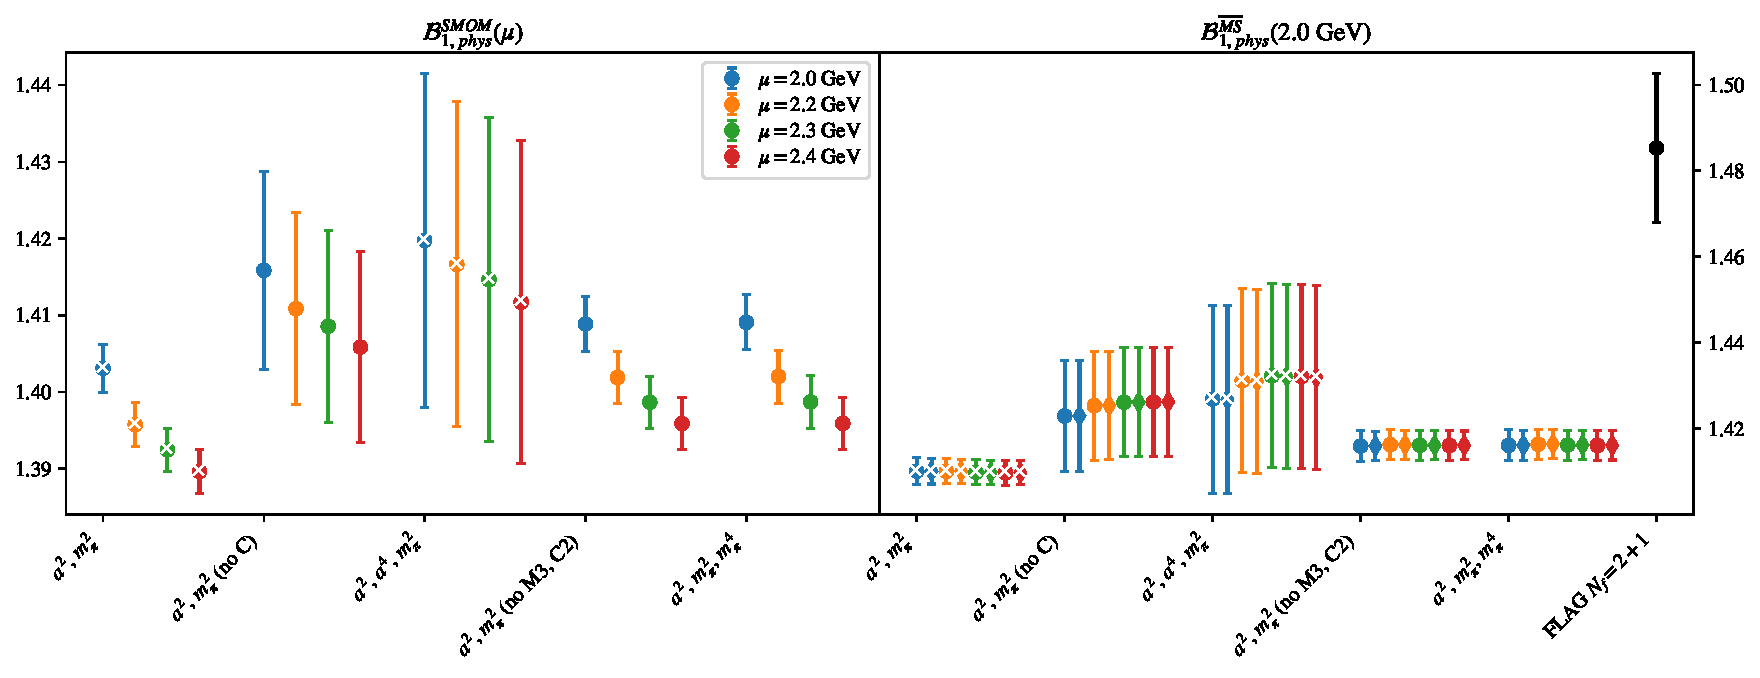
\includegraphics[page=1, width=1.1\textwidth]{VVpAA/SUSY/fit_summary_bag.pdf}
\caption{$\mathcal{B}_{1}$\\(left) $\mathcal{B}_{phys}$ in RI/SMOM scheme from fit variations (fits with $p$-value $<0.05$ marked with ``$\times$"). \\(right) $\mathcal{B}_{phys}$ in $\overline{MS}$ computed using $\mathcal{B}^{\overline{MS}} = R^{\overline{MS}\leftarrow SMOM}(2.0)\sigma_{npt}(2.0,\mu) \mathcal{B}^{SMOM}(\mu)$.}
\end{figure}
\clearpage
\begin{figure}
\centering
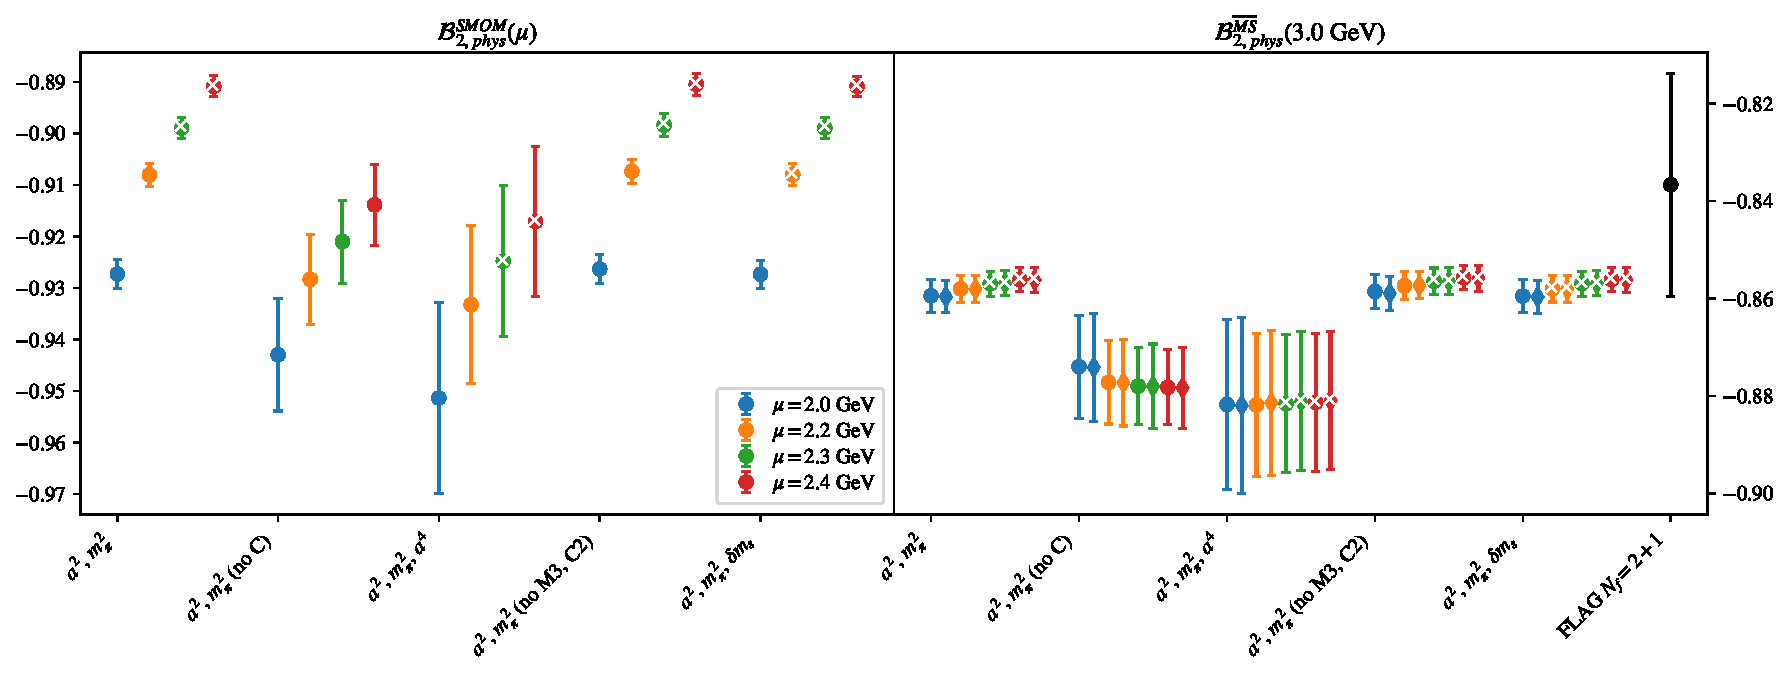
\includegraphics[page=1, width=1.1\textwidth]{VVmAA/SUSY/fit_summary_bag.pdf}
\caption{$\mathcal{B}_{2}$\\(left) $\mathcal{B}_{phys}$ in RI/SMOM scheme from fit variations (fits with $p$-value $<0.05$ marked with ``$\times$"). \\(right) $\mathcal{B}_{phys}$ in $\overline{MS}$ computed using $\mathcal{B}^{\overline{MS}} = R^{\overline{MS}\leftarrow SMOM}(3.0)\sigma_{npt}(3.0,\mu) \mathcal{B}^{SMOM}(\mu)$.}
\end{figure}
\clearpage
\begin{figure}
\centering
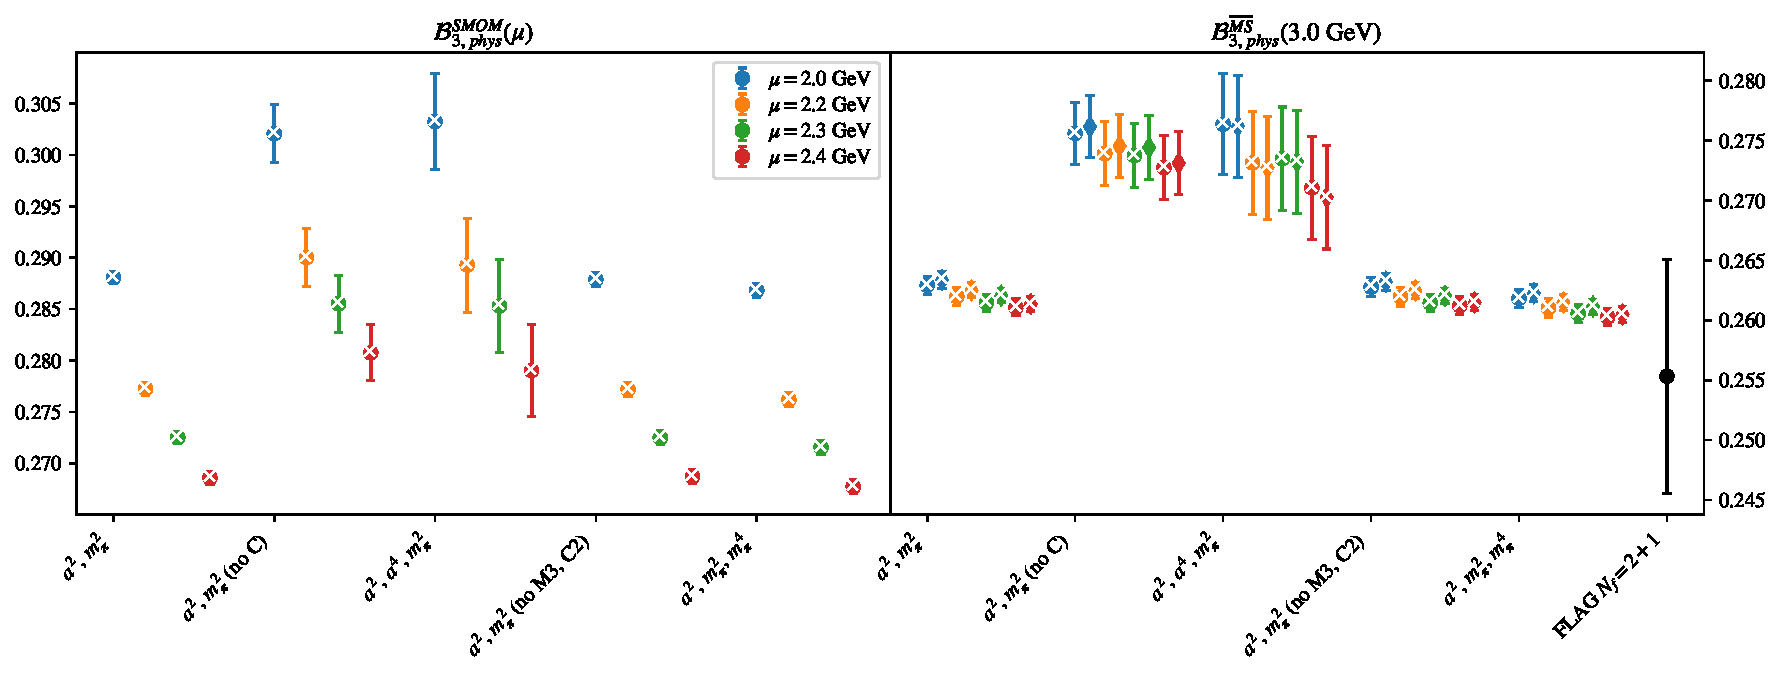
\includegraphics[page=1, width=1.1\textwidth]{SSmPP/SUSY/fit_summary_bag.pdf}
\caption{$\mathcal{B}_{3}$\\(left) $\mathcal{B}_{phys}$ in RI/SMOM scheme from fit variations (fits with $p$-value $<0.05$ marked with ``$\times$"). \\(right) $\mathcal{B}_{phys}$ in $\overline{MS}$ computed using $\mathcal{B}^{\overline{MS}} = R^{\overline{MS}\leftarrow SMOM}(3.0)\sigma_{npt}(3.0,\mu) \mathcal{B}^{SMOM}(\mu)$.}
\end{figure}
\clearpage
\begin{figure}
\centering
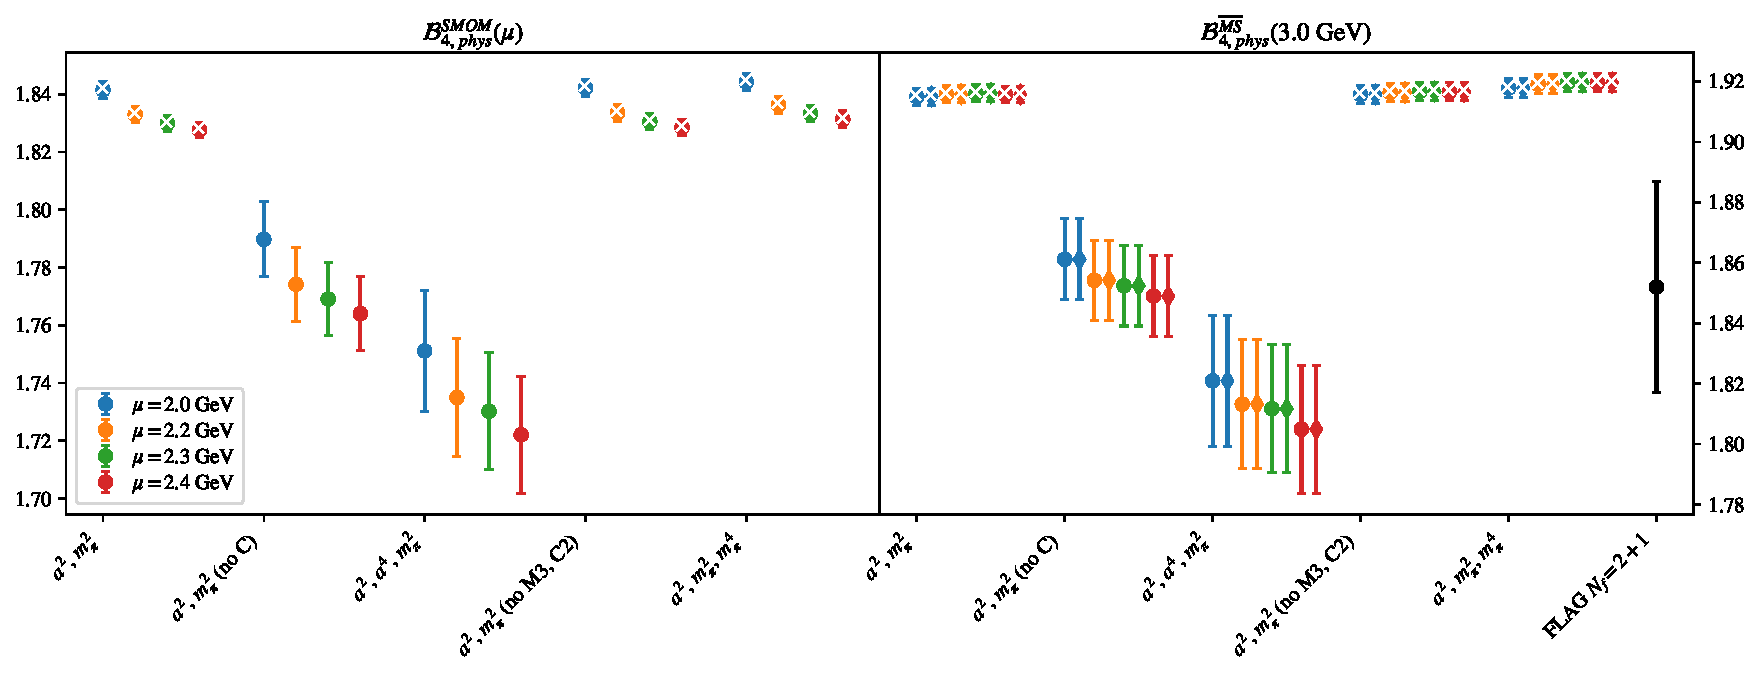
\includegraphics[page=1, width=1.1\textwidth]{SSpPP/SUSY/fit_summary_bag.pdf}
\caption{$\mathcal{B}_{4}$\\(left) $\mathcal{B}_{phys}$ in RI/SMOM scheme from fit variations (fits with $p$-value $<0.05$ marked with ``$\times$"). \\(right) $\mathcal{B}_{phys}$ in $\overline{MS}$ computed using $\mathcal{B}^{\overline{MS}} = R^{\overline{MS}\leftarrow SMOM}(3.0)\sigma_{npt}(3.0,\mu) \mathcal{B}^{SMOM}(\mu)$.}
\end{figure}
\clearpage
\begin{figure}
\centering
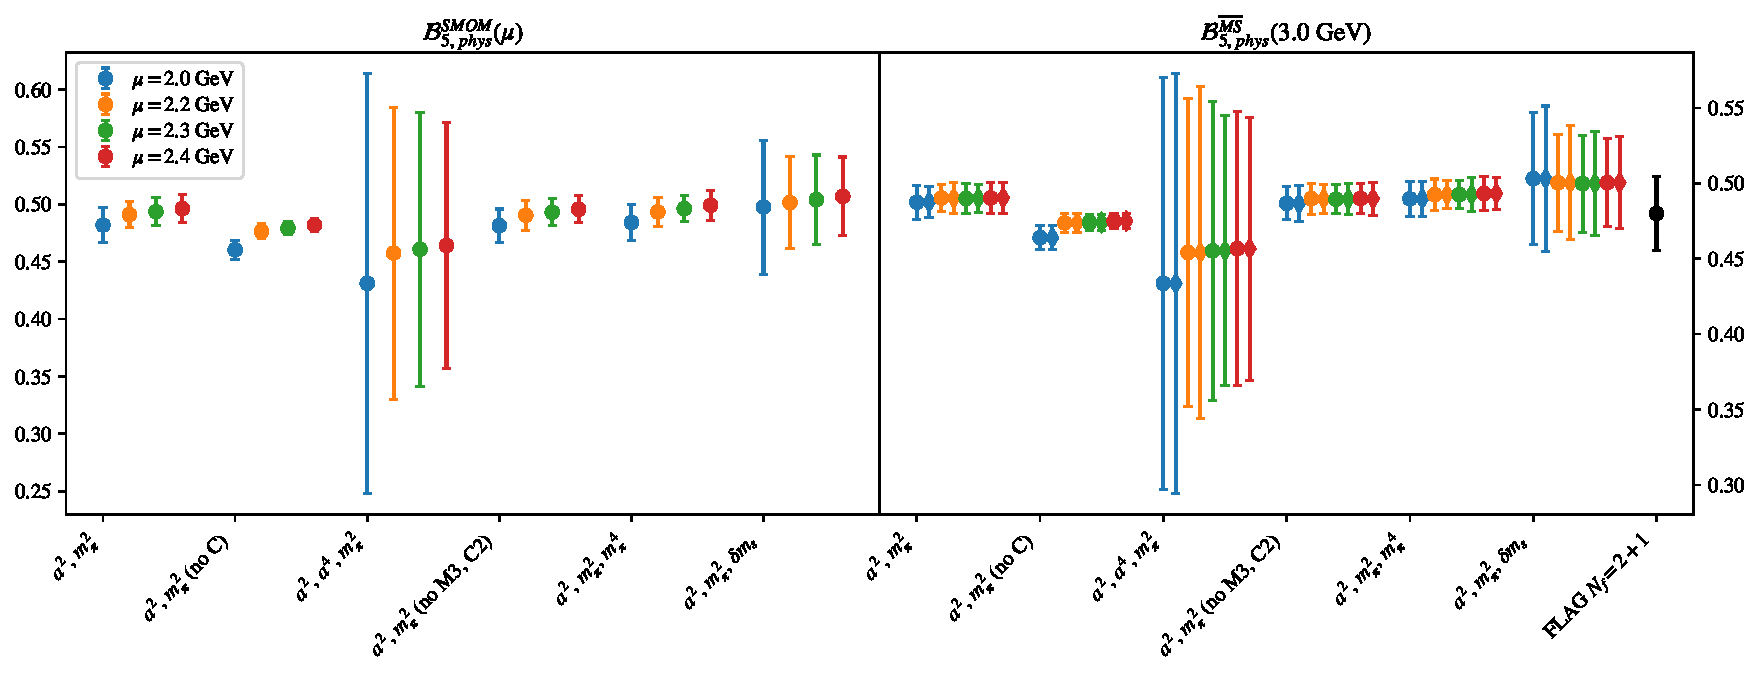
\includegraphics[page=1, width=1.1\textwidth]{TT/SUSY/fit_summary_bag.pdf}
\caption{$\mathcal{B}_{5}$\\(left) $\mathcal{B}_{phys}$ in RI/SMOM scheme from fit variations (fits with $p$-value $<0.05$ marked with ``$\times$"). \\(right) $\mathcal{B}_{phys}$ in $\overline{MS}$ computed using $\mathcal{B}^{\overline{MS}} = R^{\overline{MS}\leftarrow SMOM}(3.0)\sigma_{npt}(3.0,\mu) \mathcal{B}^{SMOM}(\mu)$.}
\end{figure}
\clearpage
\section{$\mathcal{B}_1$}
\begin{table}[h!]
\begin{center}
\begin{tabular}{|c|c|c|c|c|c|}
\hline
$\mu$ (GeV) & $a^2$, $m_\pi^2$& $a^2$, $m_\pi^2$ (no C)& $a^2$, $m_\pi^2$, $a^4$& $a^2$, $m_\pi^2$ (no M3, C2)& $a^2$, $m_\pi^2$, $\delta m_s$\\
\hline
2.0& \hyperlink{VVpAA/SUSY/bag_a2m2_20.pdf.1}{\textbf{1.4003(30)}: 2.547 (0.026)} & \hyperlink{VVpAA/SUSY/bag_a2m2noC_20.pdf.1}{\textbf{1.434(12)}: 0.255 (0.775)} & \hyperlink{VVpAA/SUSY/bag_a2a4m2_20.pdf.1}{\textbf{1.451(22)}: 1.868 (0.113)} & \hyperlink{VVpAA/SUSY/bag_a2m2mcut_20.pdf.1}{\textbf{1.4043(33)}: 2.053 (0.104)} & \hyperlink{VVpAA/SUSY/bag_a2m2delm_20.pdf.1}{\textbf{1.4005(31)}: 1.25 (0.287)}\\
2.2& \hyperlink{VVpAA/SUSY/bag_a2m2_22.pdf.1}{\textbf{1.3933(29)}: 3.059 (0.009)} & \hyperlink{VVpAA/SUSY/bag_a2m2noC_22.pdf.1}{\textbf{1.430(12)}: 0.288 (0.75)} & \hyperlink{VVpAA/SUSY/bag_a2a4m2_22.pdf.1}{\textbf{1.450(22)}: 2.131 (0.074)} & \hyperlink{VVpAA/SUSY/bag_a2m2mcut_22.pdf.1}{\textbf{1.3976(32)}: 2.518 (0.056)} & \hyperlink{VVpAA/SUSY/bag_a2m2delm_22.pdf.1}{\textbf{1.3936(31)}: 1.336 (0.254)}\\
2.3& \hyperlink{VVpAA/SUSY/bag_a2m2_23.pdf.1}{\textbf{1.3899(29)}: 3.366 (0.005)} & \hyperlink{VVpAA/SUSY/bag_a2m2noC_23.pdf.1}{\textbf{1.429(12)}: 0.33 (0.719)} & \hyperlink{VVpAA/SUSY/bag_a2a4m2_23.pdf.1}{\textbf{1.448(22)}: 2.397 (0.048)} & \hyperlink{VVpAA/SUSY/bag_a2m2mcut_23.pdf.1}{\textbf{1.3944(33)}: 2.771 (0.04)} & \hyperlink{VVpAA/SUSY/bag_a2m2delm_23.pdf.1}{\textbf{1.3902(31)}: 1.529 (0.191)}\\
2.4& \hyperlink{VVpAA/SUSY/bag_a2m2_24.pdf.1}{\textbf{1.3868(29)}: 3.569 (0.003)} & \hyperlink{VVpAA/SUSY/bag_a2m2noC_24.pdf.1}{\textbf{1.426(12)}: 0.347 (0.707)} & \hyperlink{VVpAA/SUSY/bag_a2a4m2_24.pdf.1}{\textbf{1.446(22)}: 2.594 (0.035)} & \hyperlink{VVpAA/SUSY/bag_a2m2mcut_24.pdf.1}{\textbf{1.3915(33)}: 2.877 (0.035)} & \hyperlink{VVpAA/SUSY/bag_a2m2delm_24.pdf.1}{\textbf{1.3872(31)}: 1.647 (0.159)}\\
\hline
\end{tabular}
\caption{Physical point value from chiral and continuum extrapolation at renormalisation scale $\mu$. Entries are \textbf{value(error)}: $\chi^2/\text{DOF}$ ($p$-value).}
\end{center}
\end{table}
\begin{table}[h!]
\begin{center}
\begin{tabular}{|c c|c|c|c|c|c|}
\hline
$\mu$ (GeV) &  & $a^2$, $m_\pi^2$& $a^2$, $m_\pi^2$ (no C)& $a^2$, $m_\pi^2$, $a^4$& $a^2$, $m_\pi^2$ (no M3, C2)& $a^2$, $m_\pi^2$, $\delta m_s$\\
\hline
\multirow{3}{0.5in}{2.0} & $\alpha$ & 0.145(10)& -0.045(75)& -0.32(20)& 0.133(11)& 0.149(11)\\
 & $\beta$ & 0.00413(23)& 0.00353(43)& 0.00440(26)& 0.00349(37)& 0.00539(47)\\
 & $\gamma$ &  &  & 0.96(41)&  & -0.049(15)\\
\hline
\multirow{3}{0.5in}{2.2} & $\alpha$ & 0.149(10)& -0.060(75)& -0.37(20)& 0.136(11)& 0.153(11)\\
 & $\beta$ & 0.00400(22)& 0.00338(42)& 0.00430(25)& 0.00331(36)& 0.00540(46)\\
 & $\gamma$ &  &  & 1.07(41)&  & -0.054(16)\\
\hline
\multirow{3}{0.5in}{2.3} & $\alpha$ & 0.152(10)& -0.067(75)& -0.39(20)& 0.138(11)& 0.156(11)\\
 & $\beta$ & 0.00396(22)& 0.00330(41)& 0.00427(25)& 0.00324(36)& 0.00540(46)\\
 & $\gamma$ &  &  & 1.10(41)&  & -0.056(15)\\
\hline
\multirow{3}{0.5in}{2.4} & $\alpha$ & 0.154(10)& -0.068(74)& -0.40(20)& 0.139(11)& 0.157(11)\\
 & $\beta$ & 0.00393(22)& 0.00325(41)& 0.00425(25)& 0.00319(35)& 0.00541(46)\\
 & $\gamma$ &  &  & 1.12(41)&  & -0.057(15)\\
\hline
\end{tabular}
\caption{Fit values of coefficients in $Q = Q_{phys} + \mathbf{\alpha} a^2 + \mathbf{\beta}\left(\frac{m_\pi^2}{f_\pi^2}-\frac{m_{\pi,PDG}^2}{f_\pi^2}\right) + \gamma(\ldots)$}
\end{center}
\end{table}
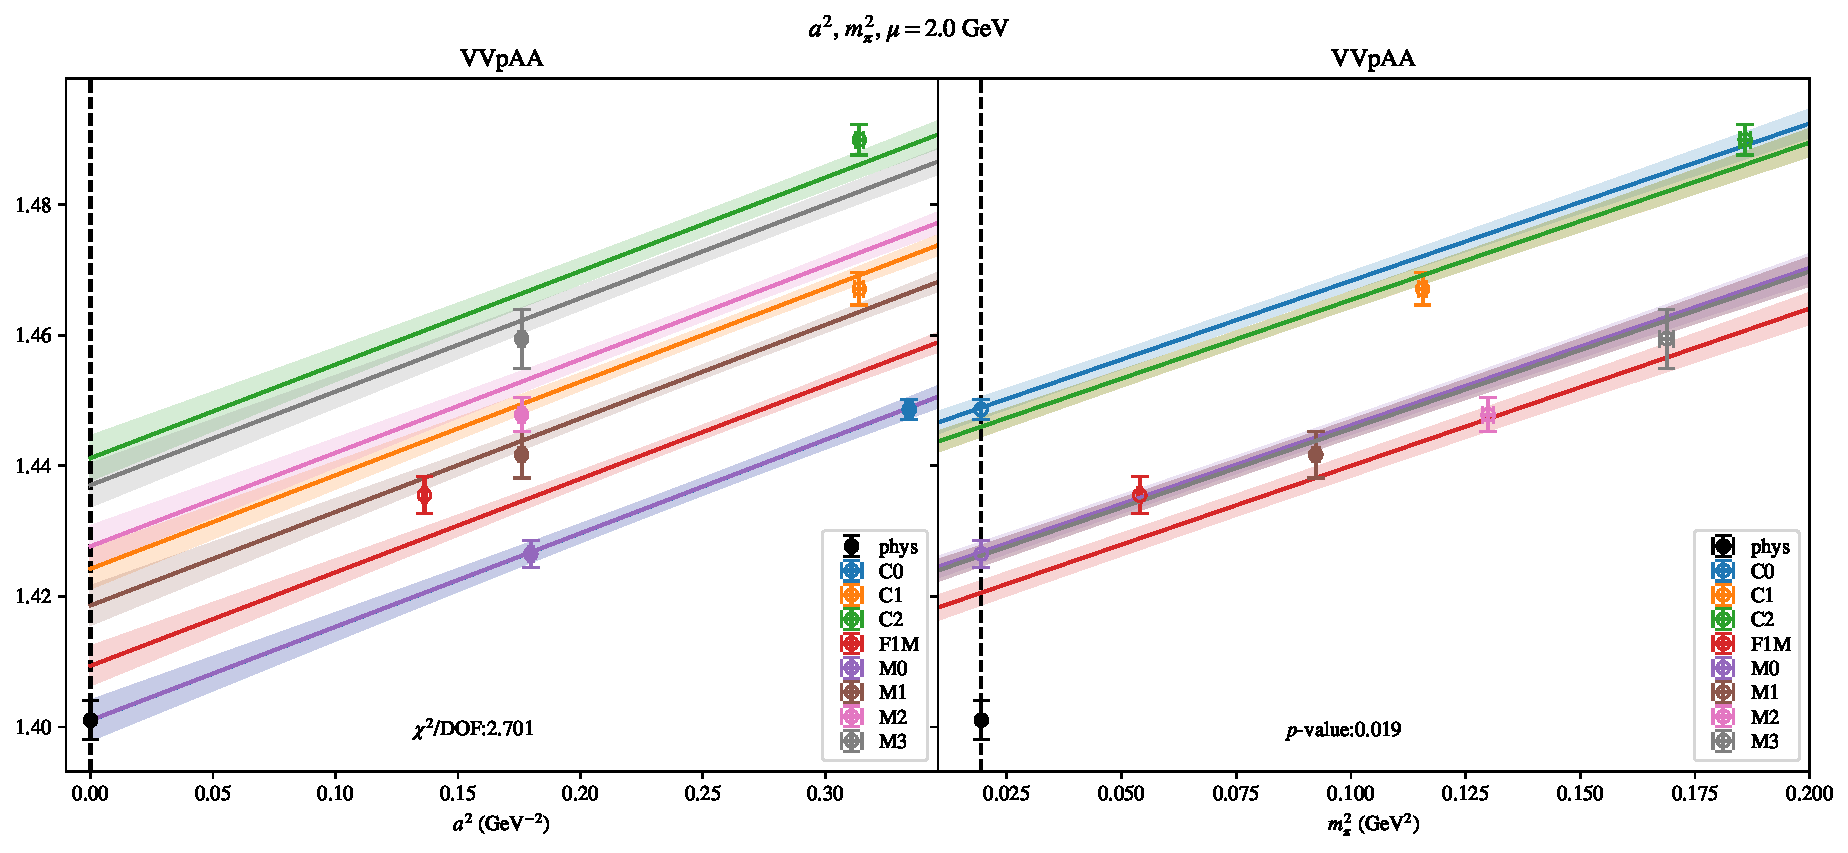
\includepdf[link, pages=-]{VVpAA/SUSY/bag_a2m2_20.pdf}
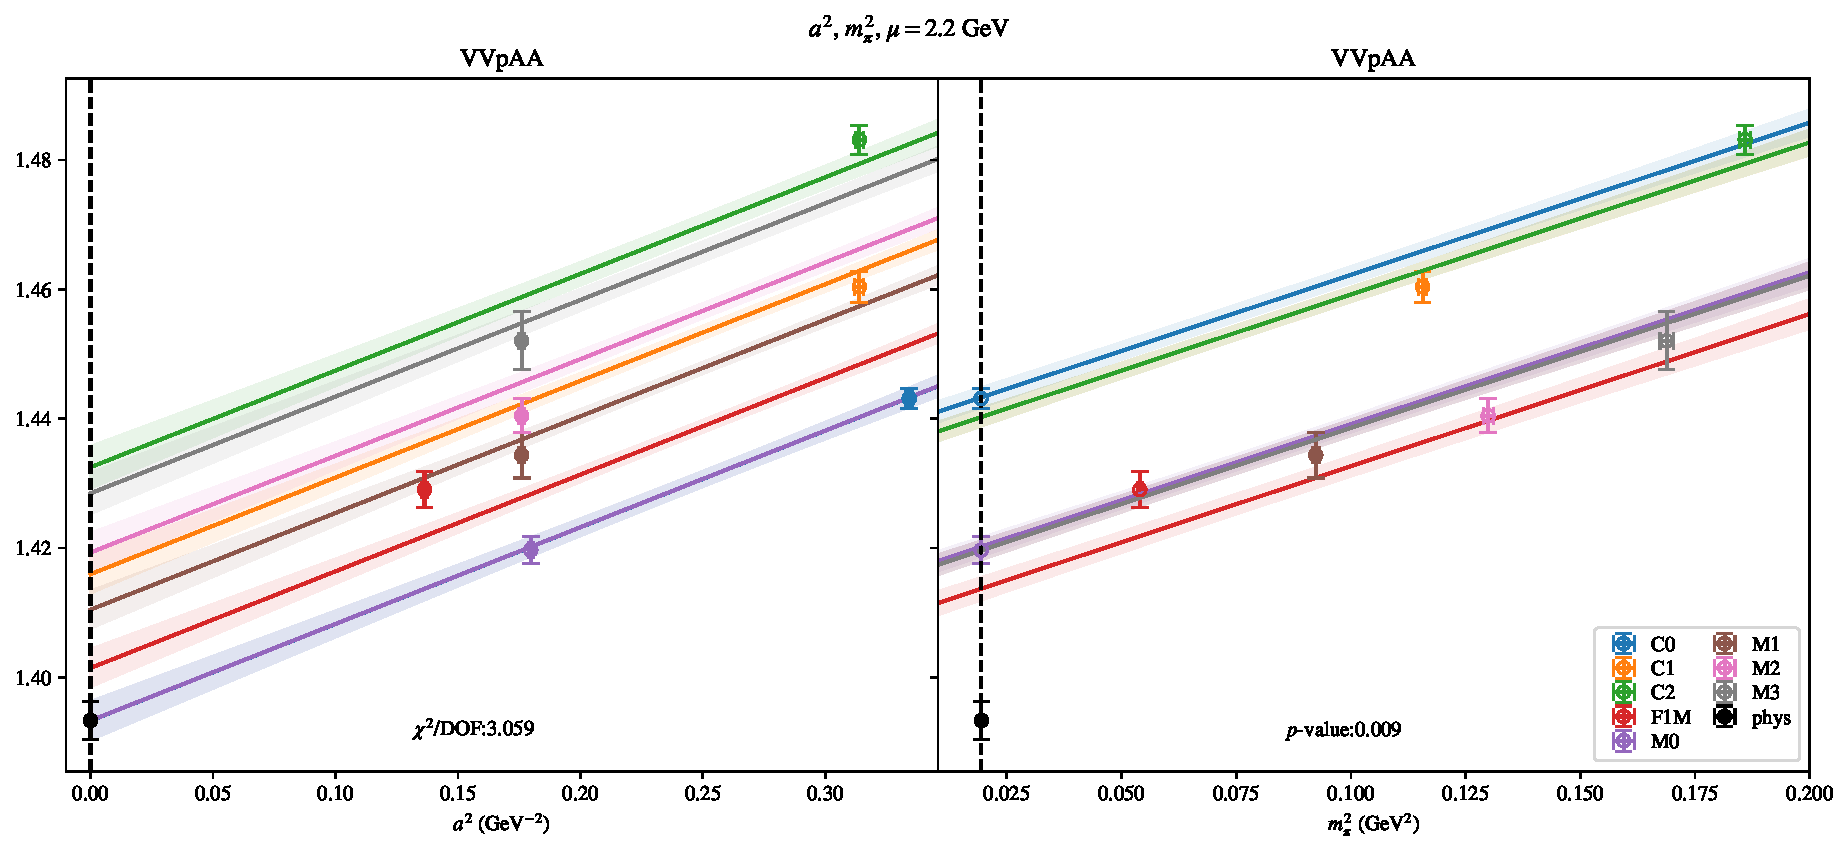
\includepdf[link, pages=-]{VVpAA/SUSY/bag_a2m2_22.pdf}
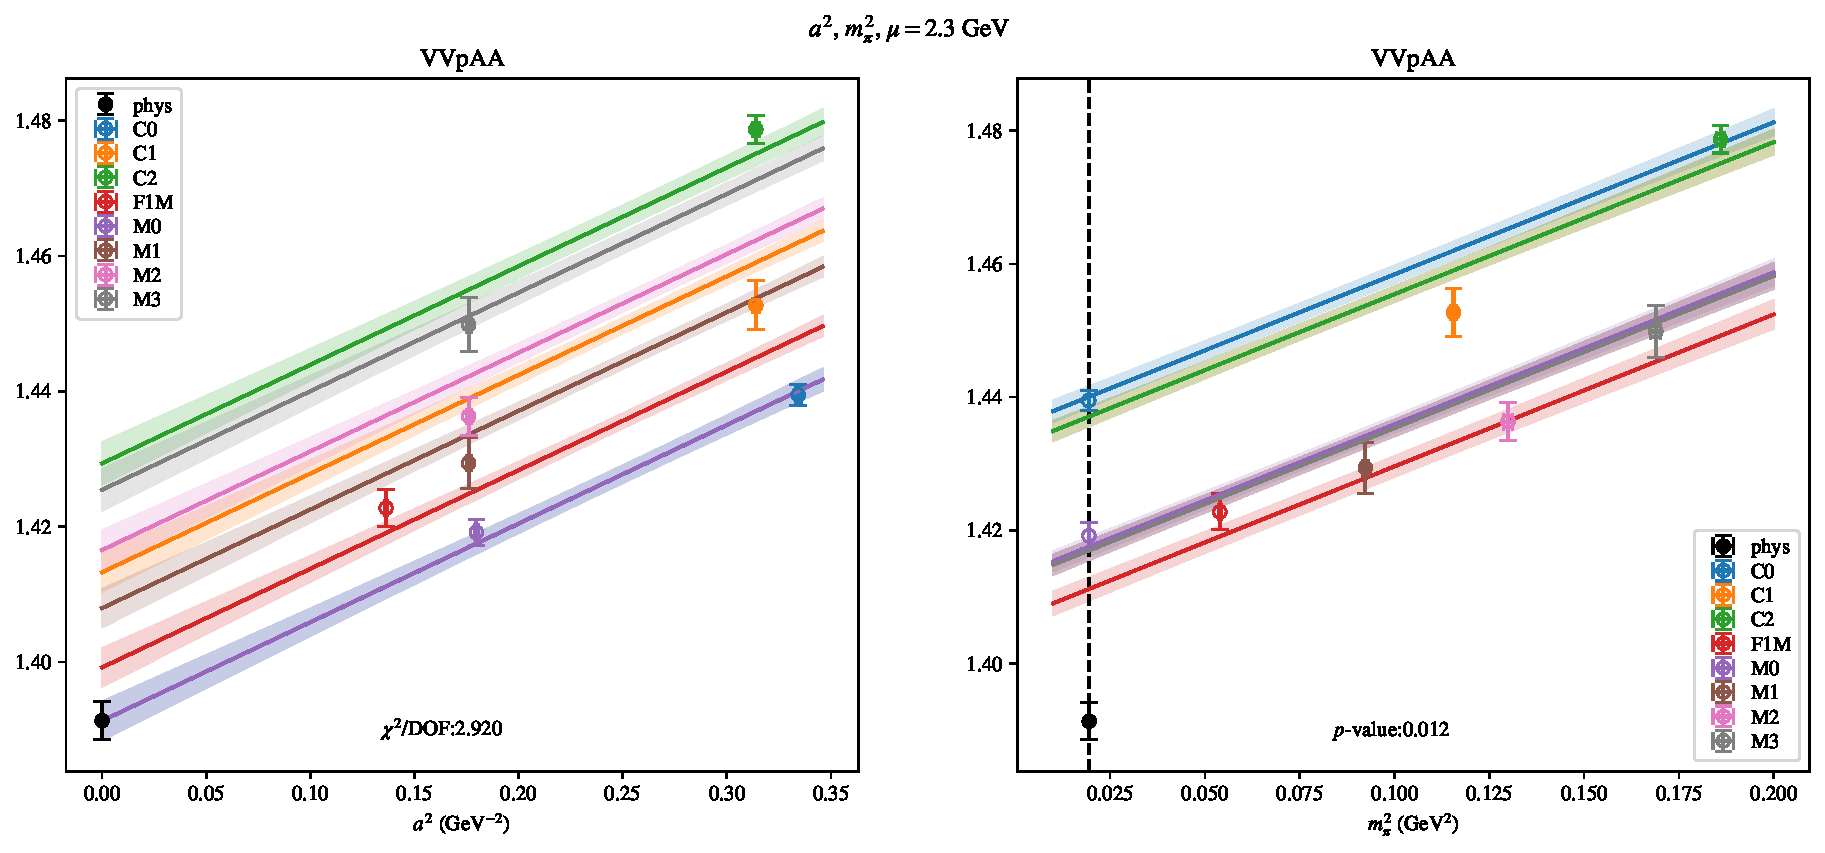
\includepdf[link, pages=-]{VVpAA/SUSY/bag_a2m2_23.pdf}
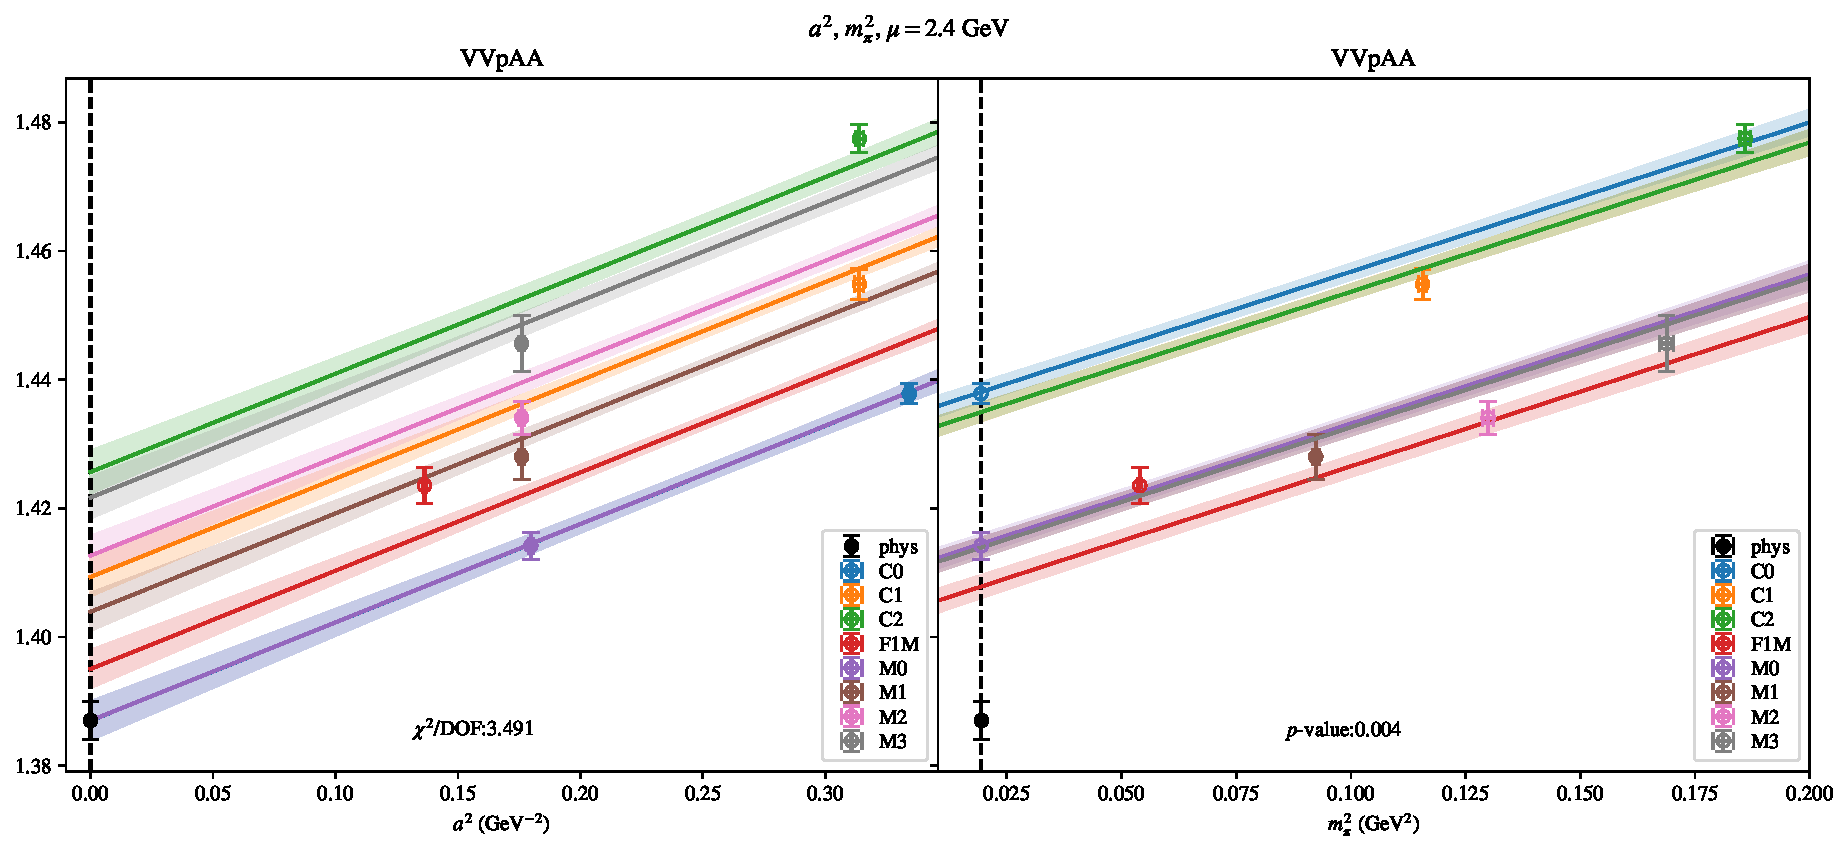
\includepdf[link, pages=-]{VVpAA/SUSY/bag_a2m2_24.pdf}
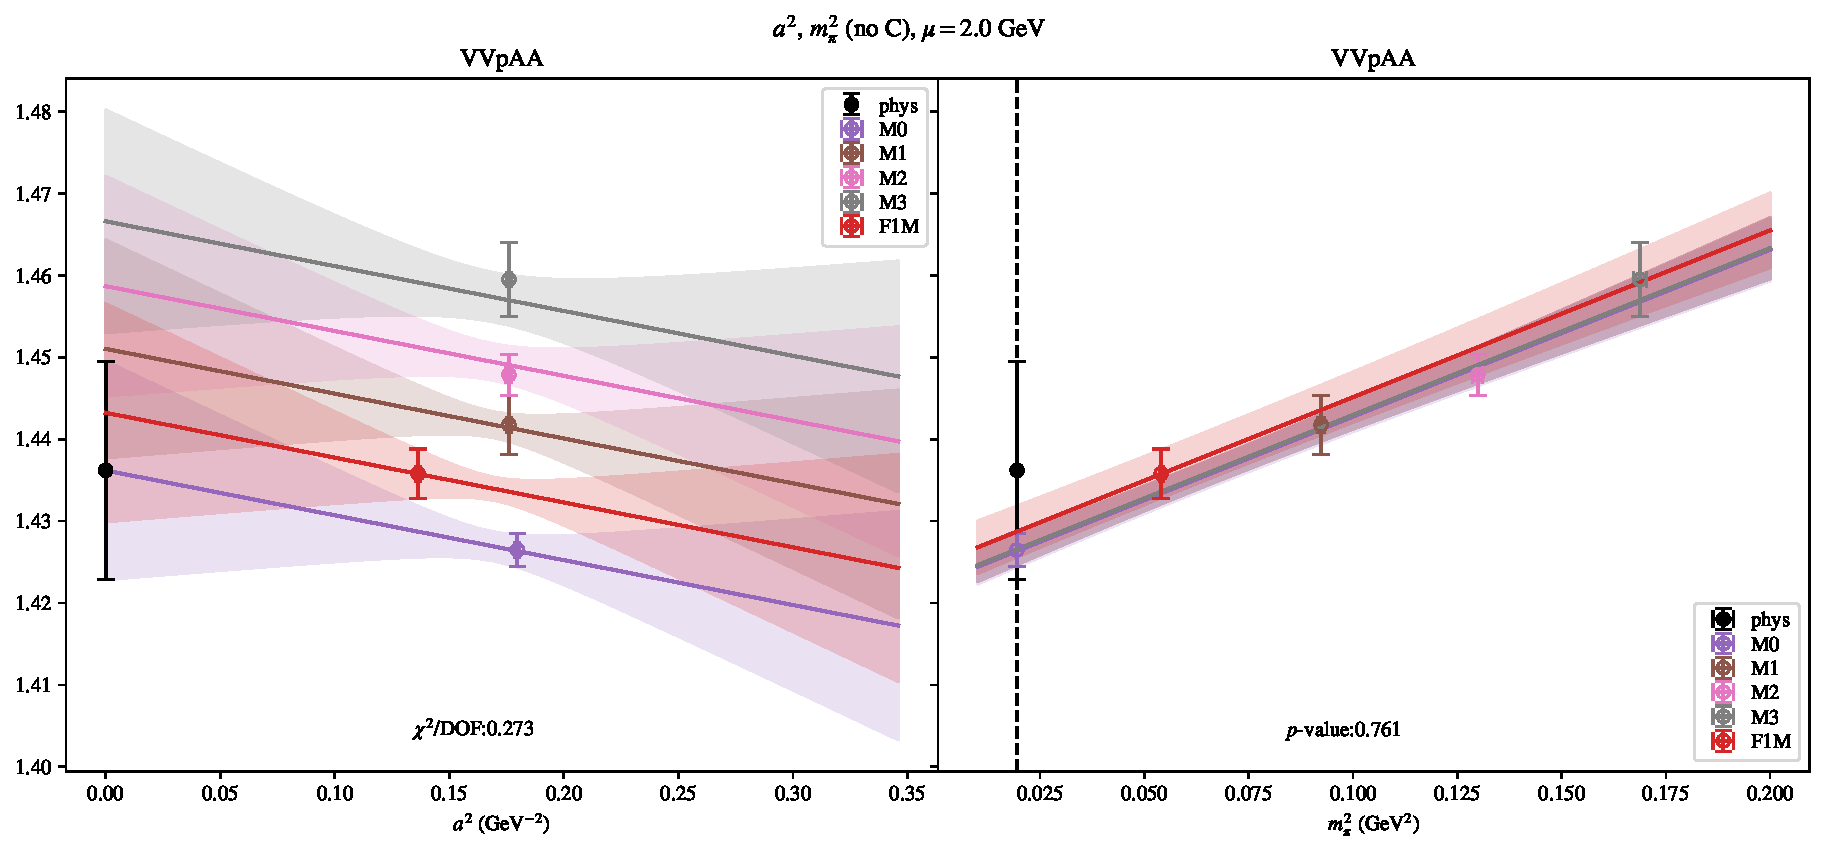
\includepdf[link, pages=-]{VVpAA/SUSY/bag_a2m2noC_20.pdf}
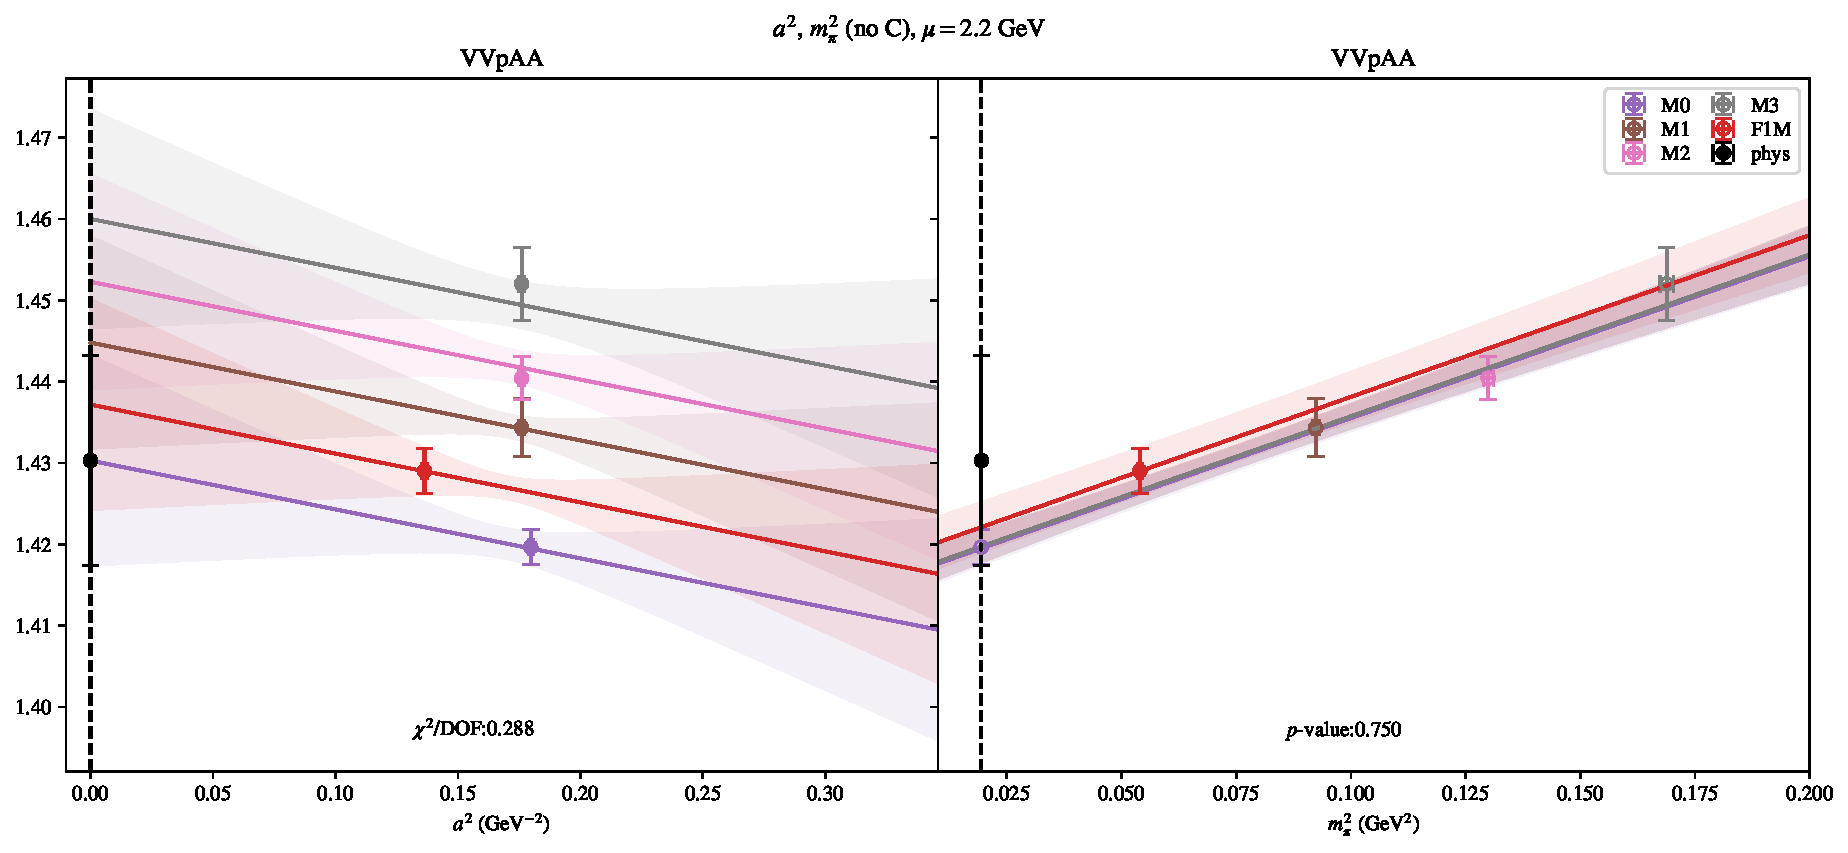
\includepdf[link, pages=-]{VVpAA/SUSY/bag_a2m2noC_22.pdf}
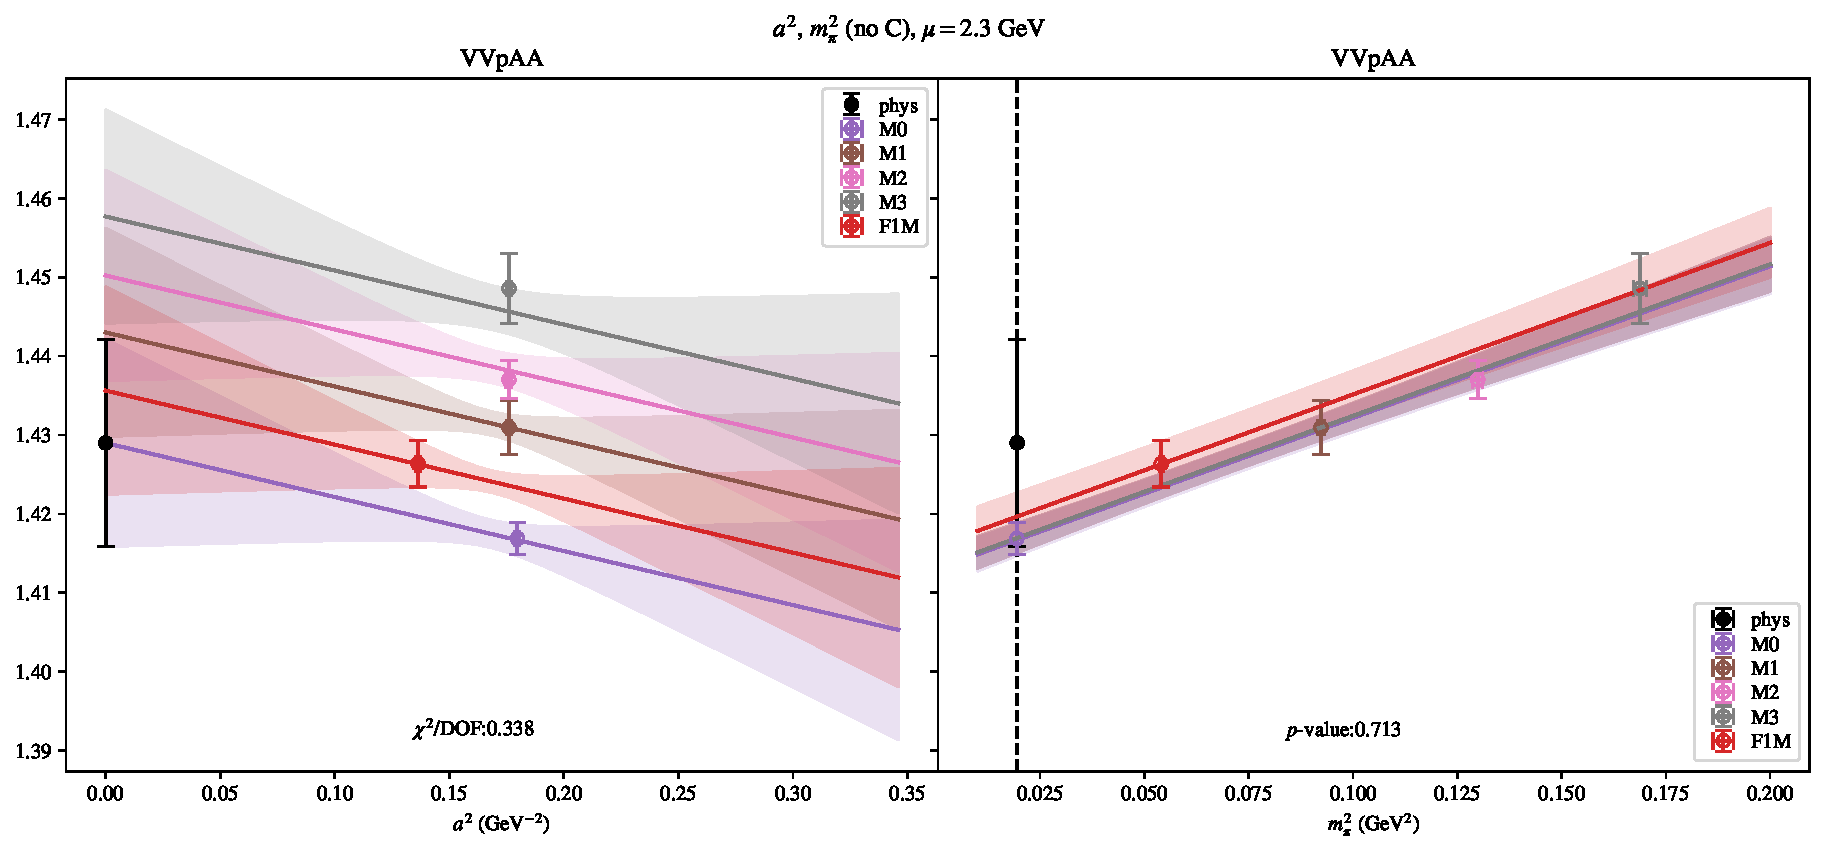
\includepdf[link, pages=-]{VVpAA/SUSY/bag_a2m2noC_23.pdf}
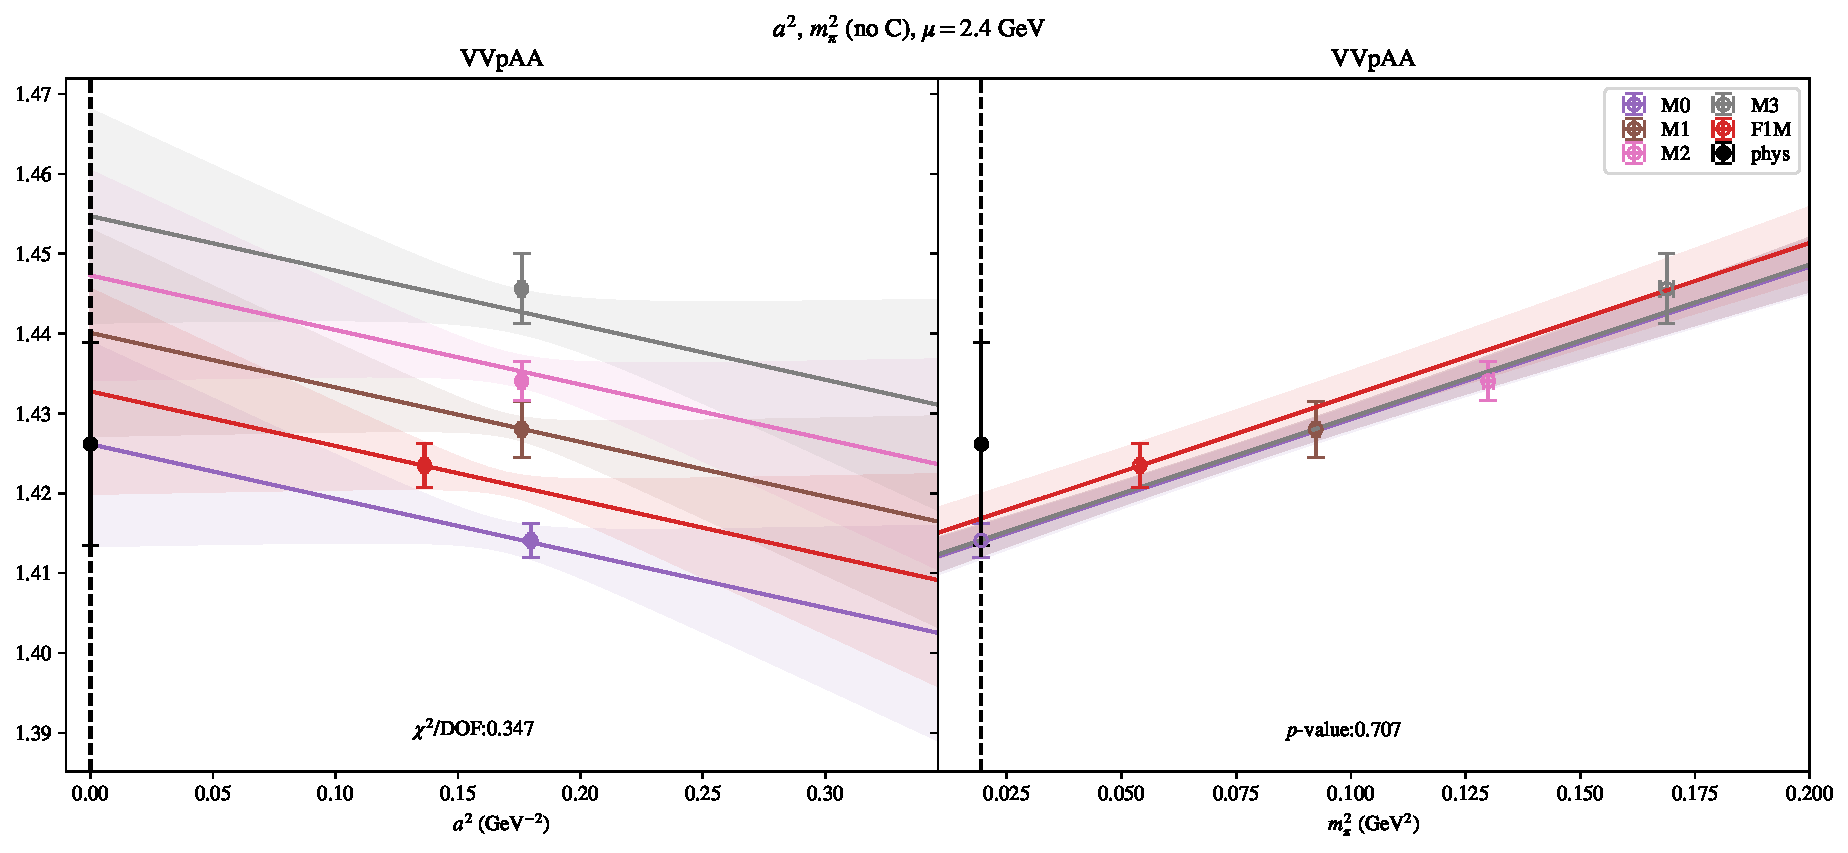
\includepdf[link, pages=-]{VVpAA/SUSY/bag_a2m2noC_24.pdf}
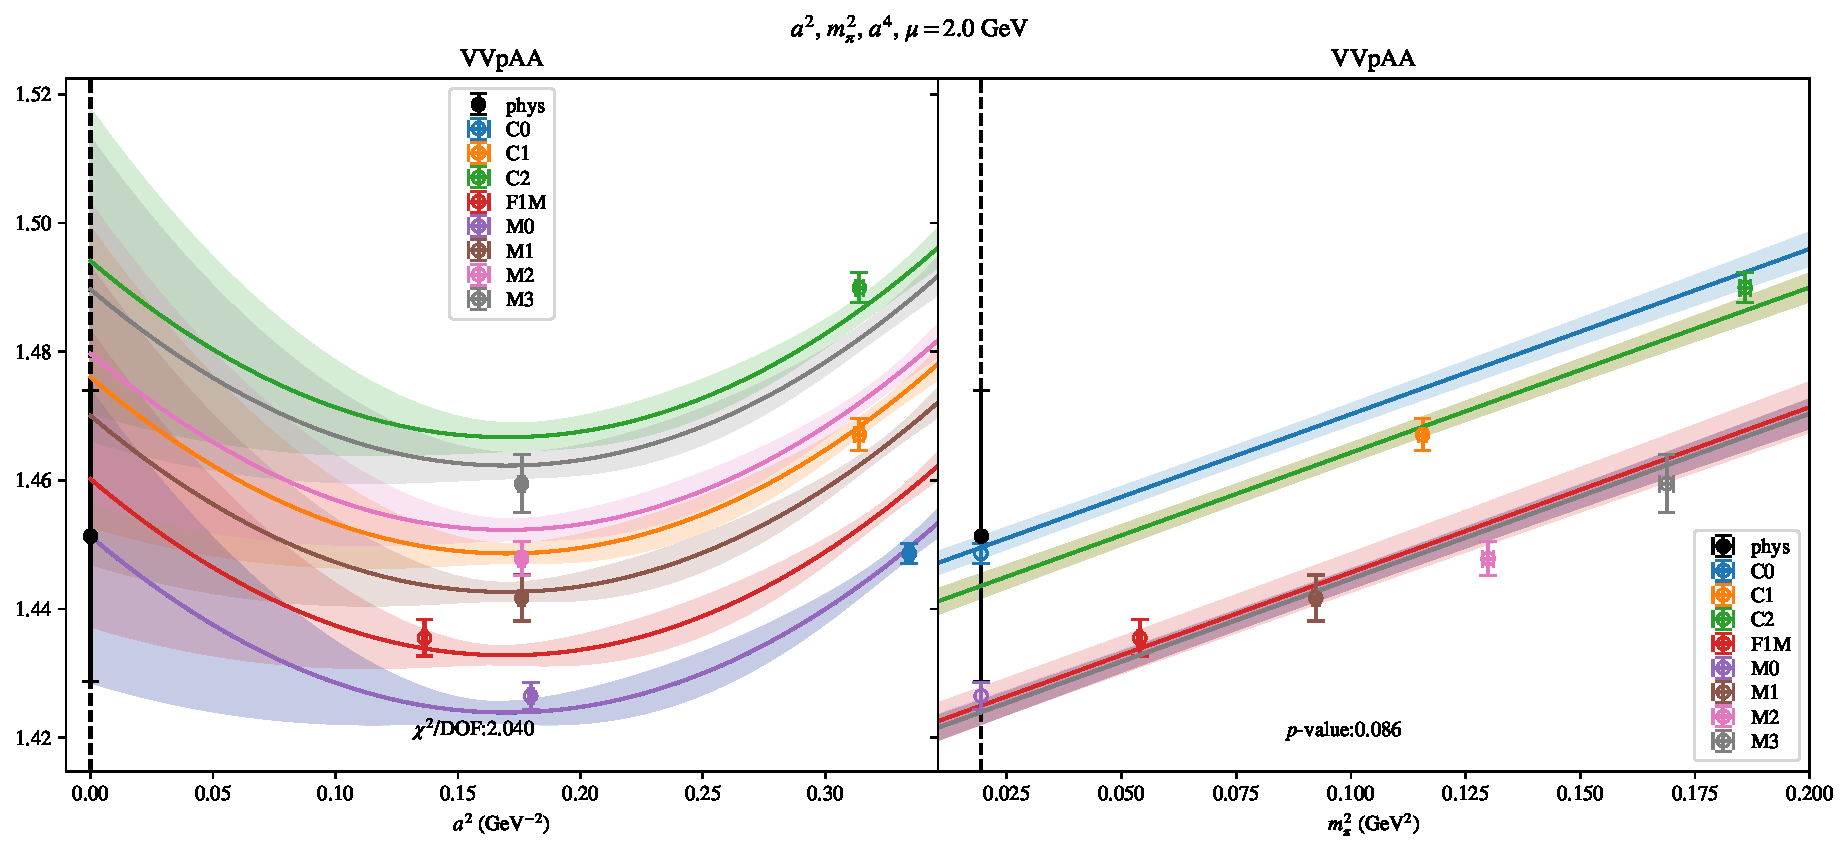
\includepdf[link, pages=-]{VVpAA/SUSY/bag_a2a4m2_20.pdf}
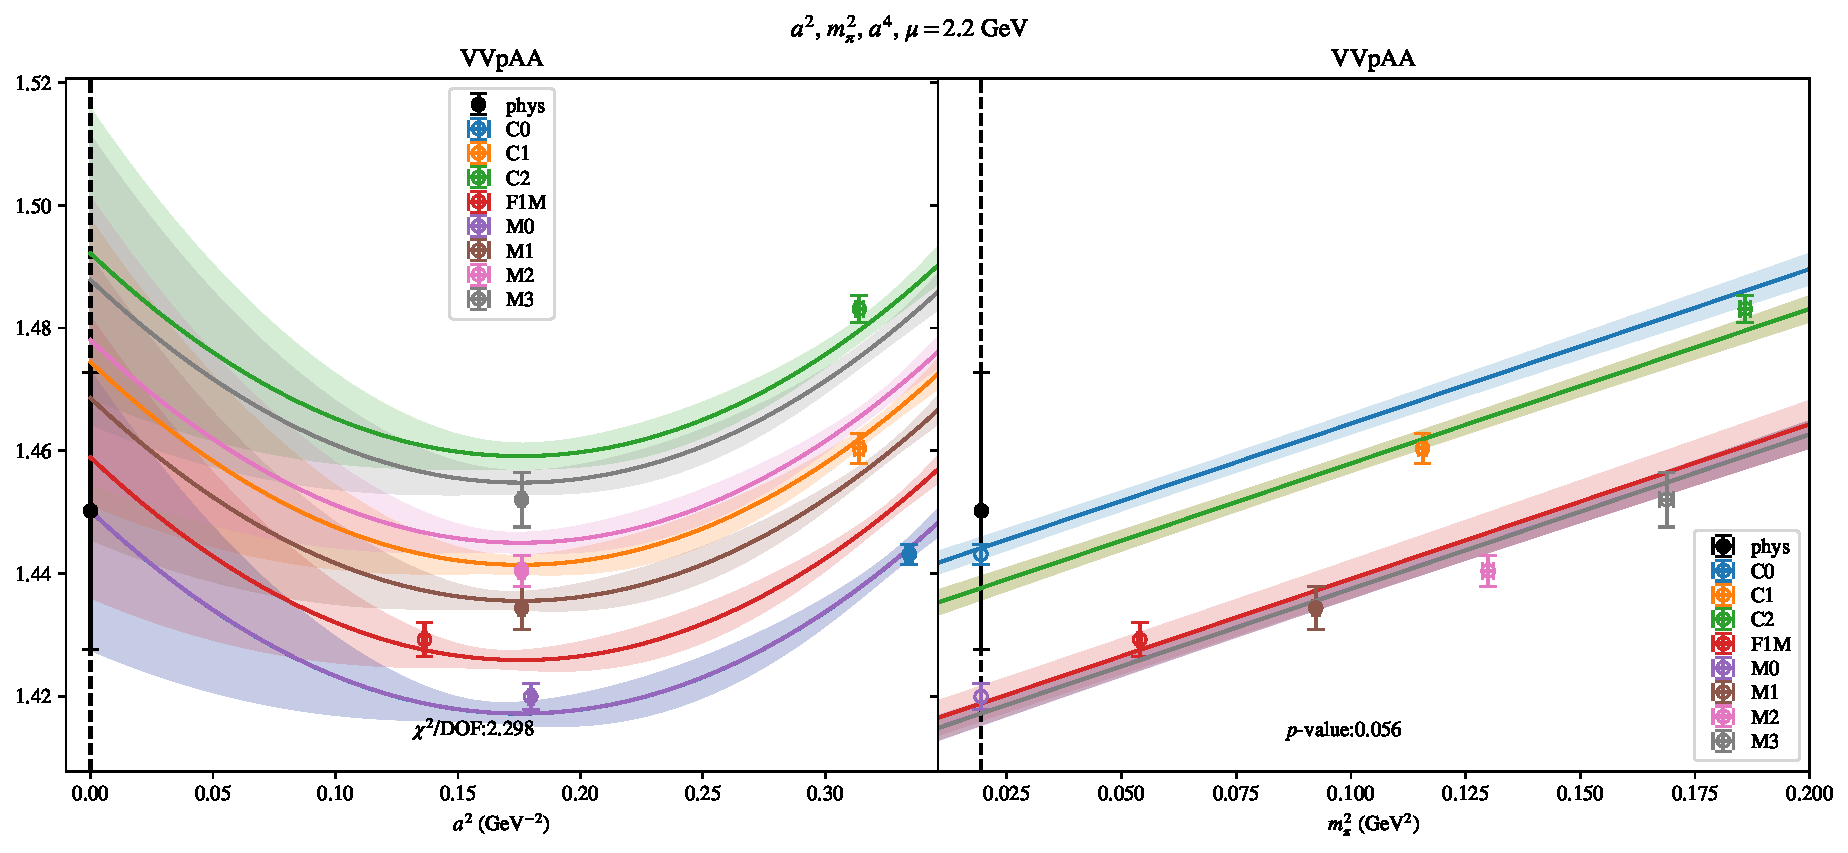
\includepdf[link, pages=-]{VVpAA/SUSY/bag_a2a4m2_22.pdf}
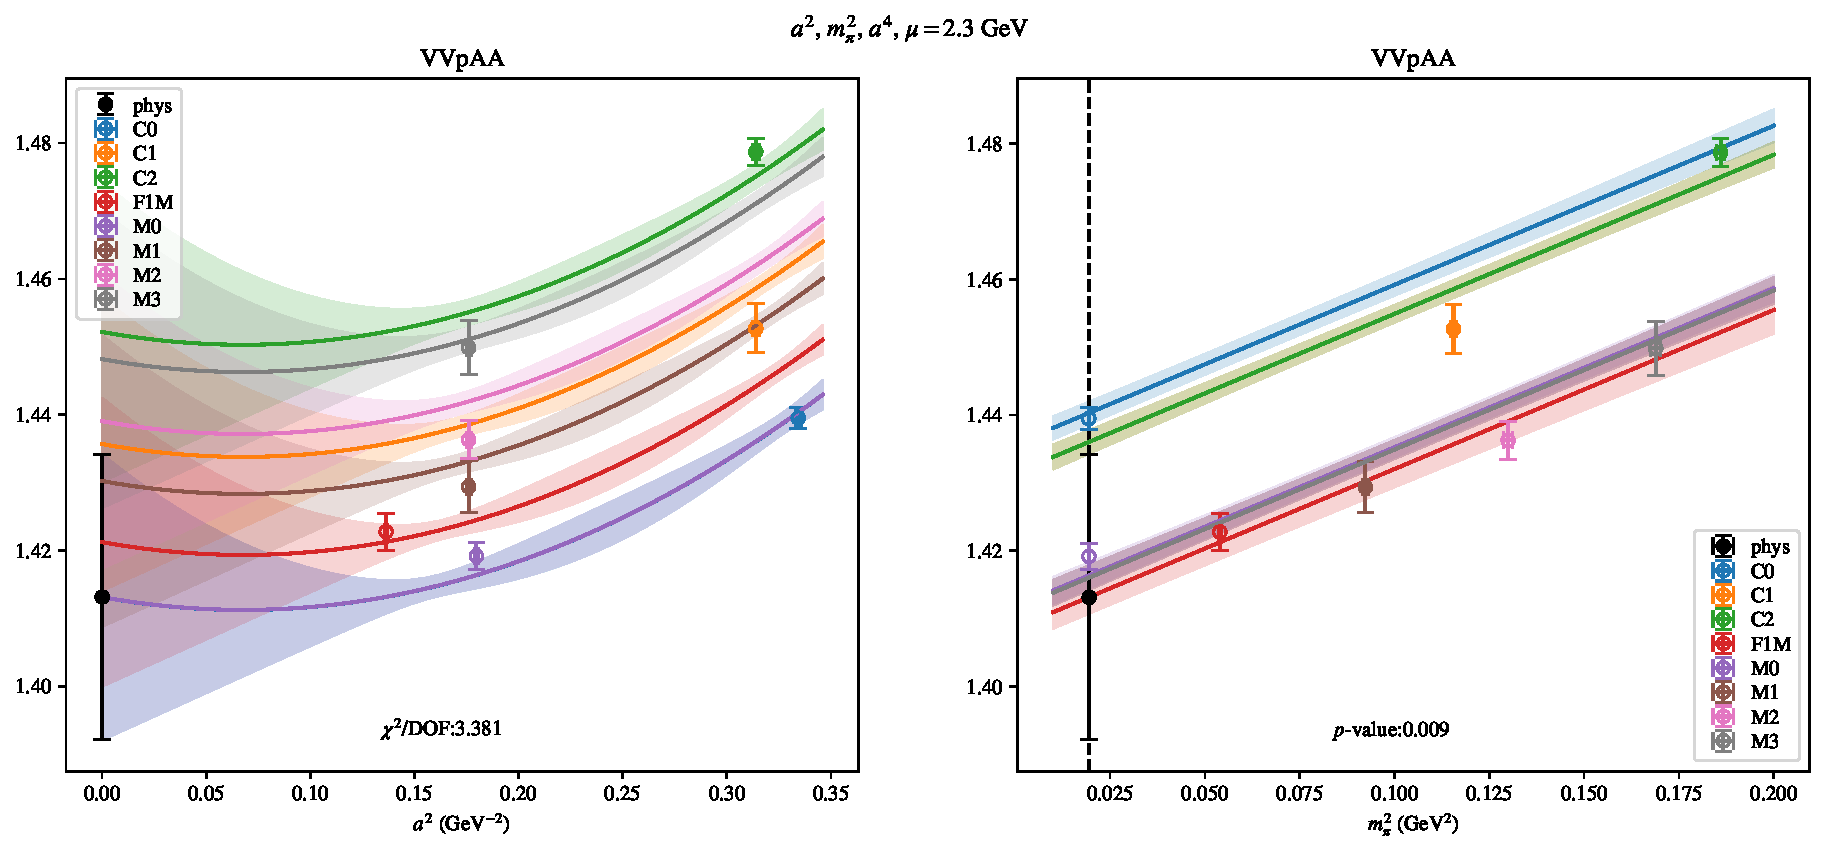
\includepdf[link, pages=-]{VVpAA/SUSY/bag_a2a4m2_23.pdf}
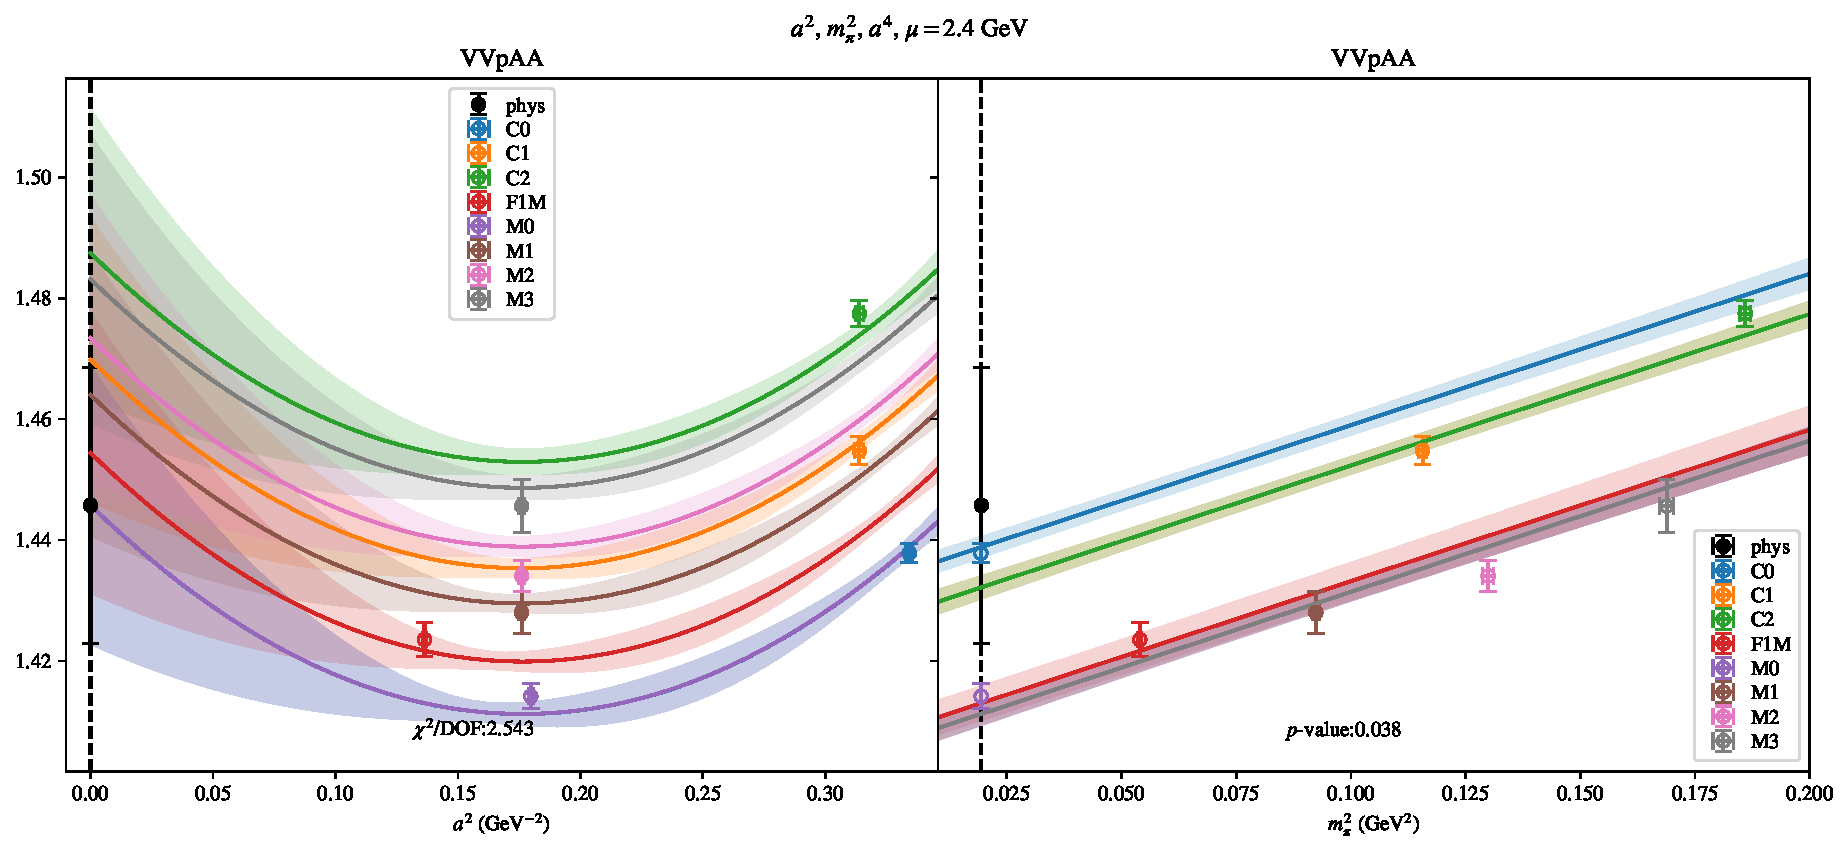
\includepdf[link, pages=-]{VVpAA/SUSY/bag_a2a4m2_24.pdf}
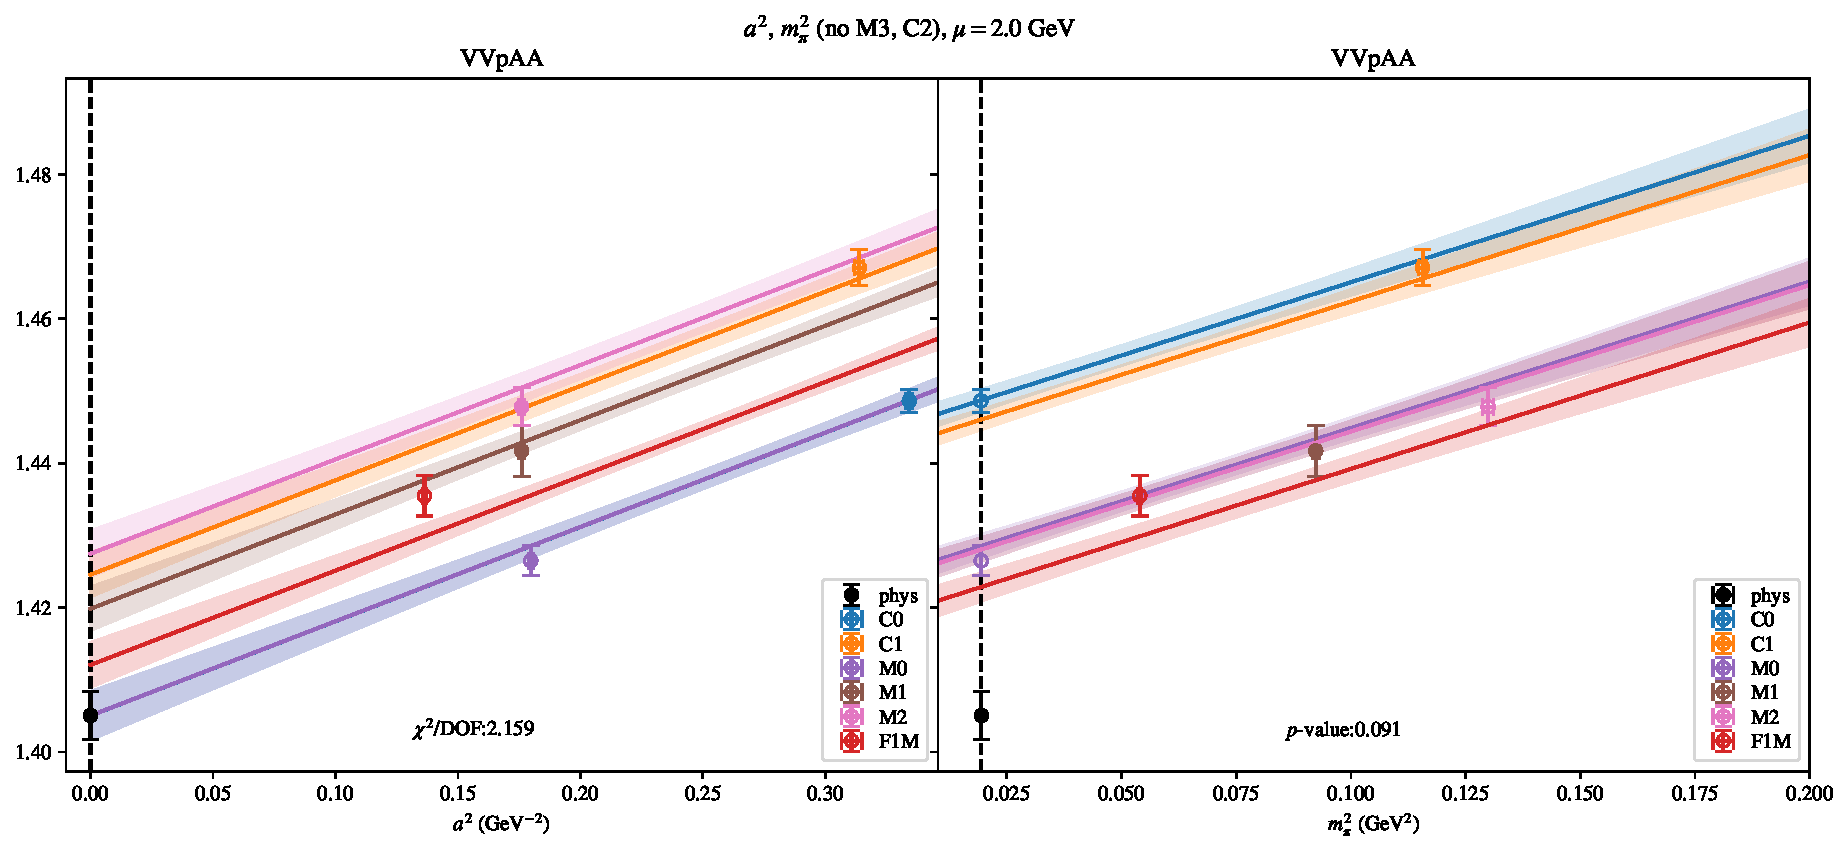
\includepdf[link, pages=-]{VVpAA/SUSY/bag_a2m2mcut_20.pdf}
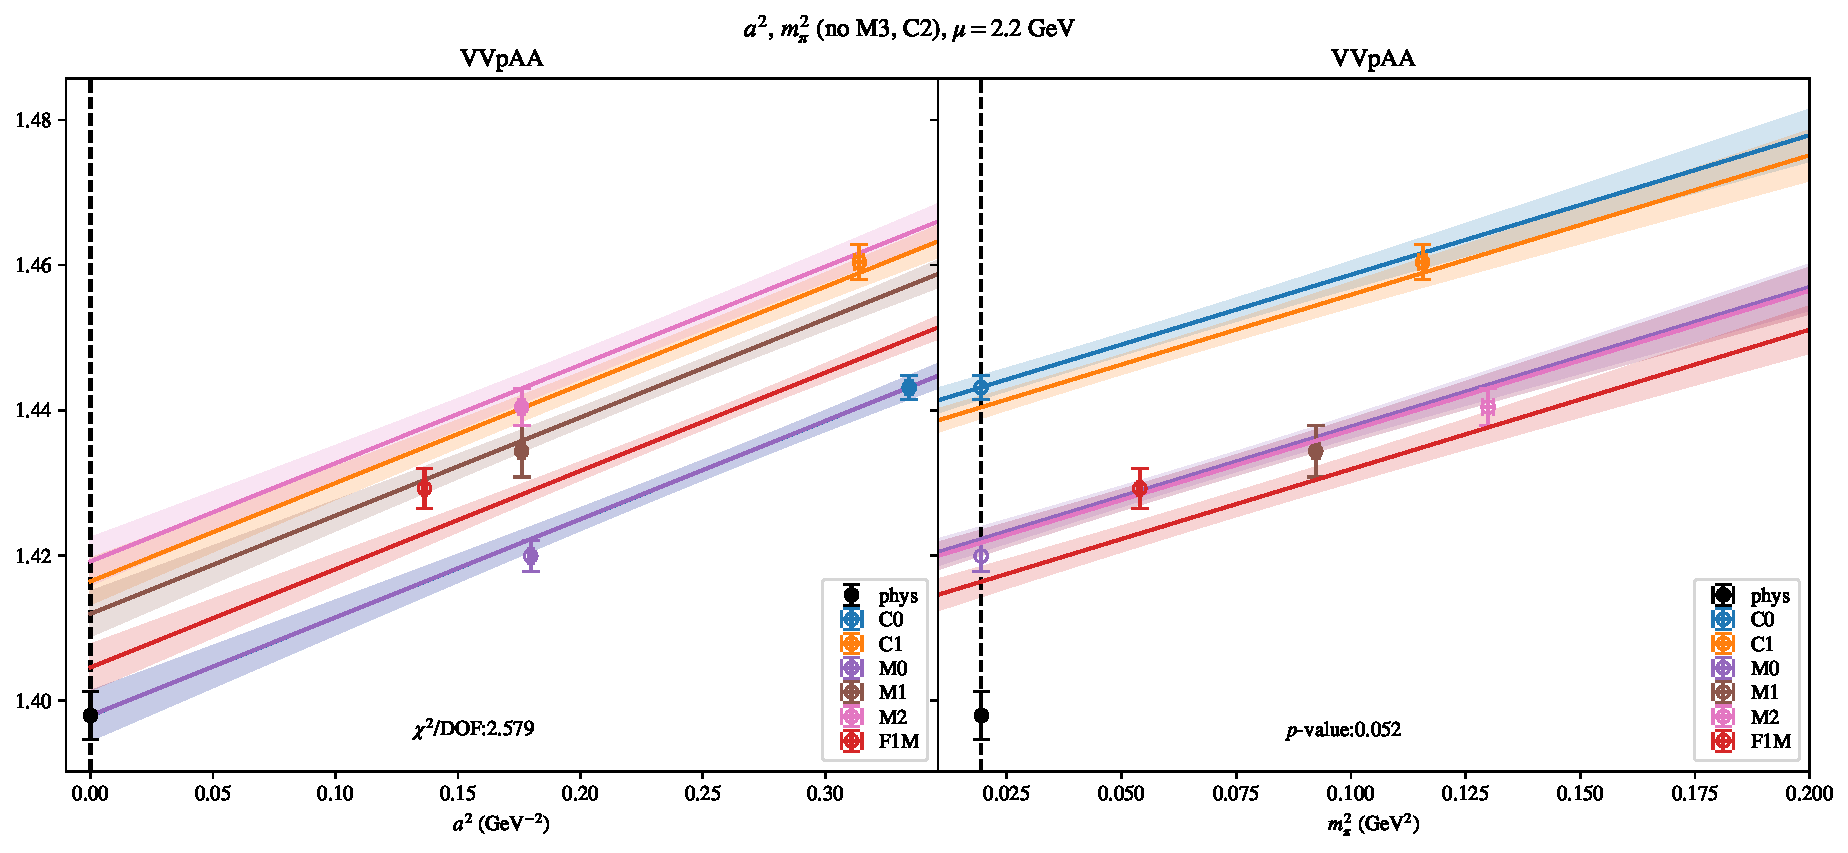
\includepdf[link, pages=-]{VVpAA/SUSY/bag_a2m2mcut_22.pdf}
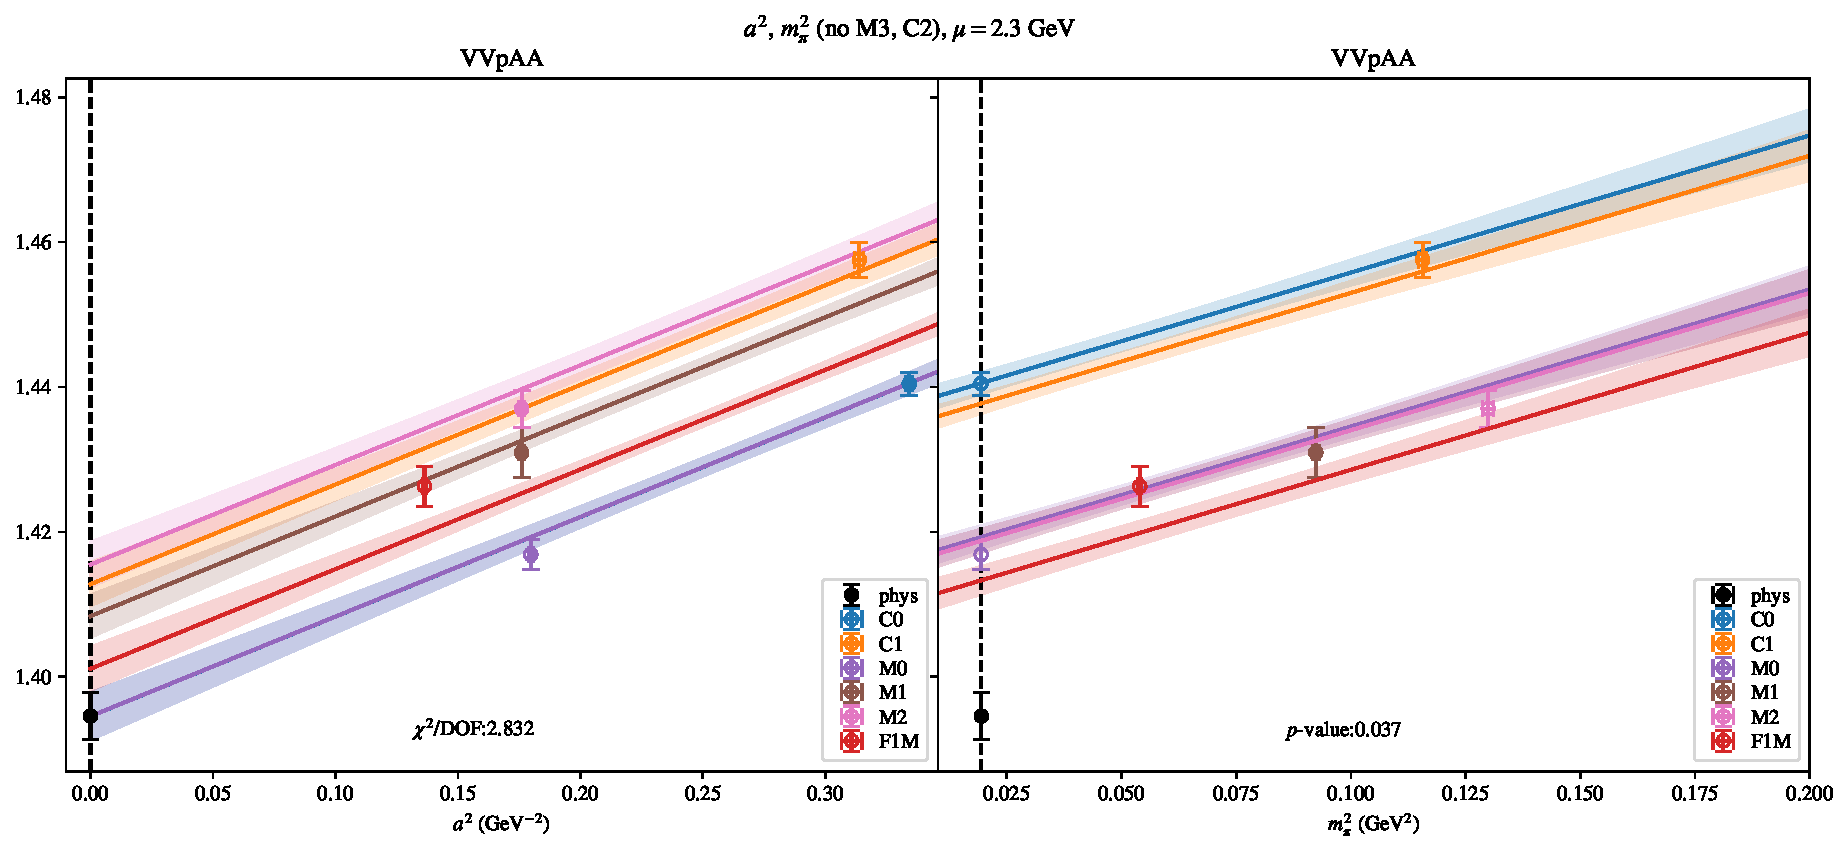
\includepdf[link, pages=-]{VVpAA/SUSY/bag_a2m2mcut_23.pdf}
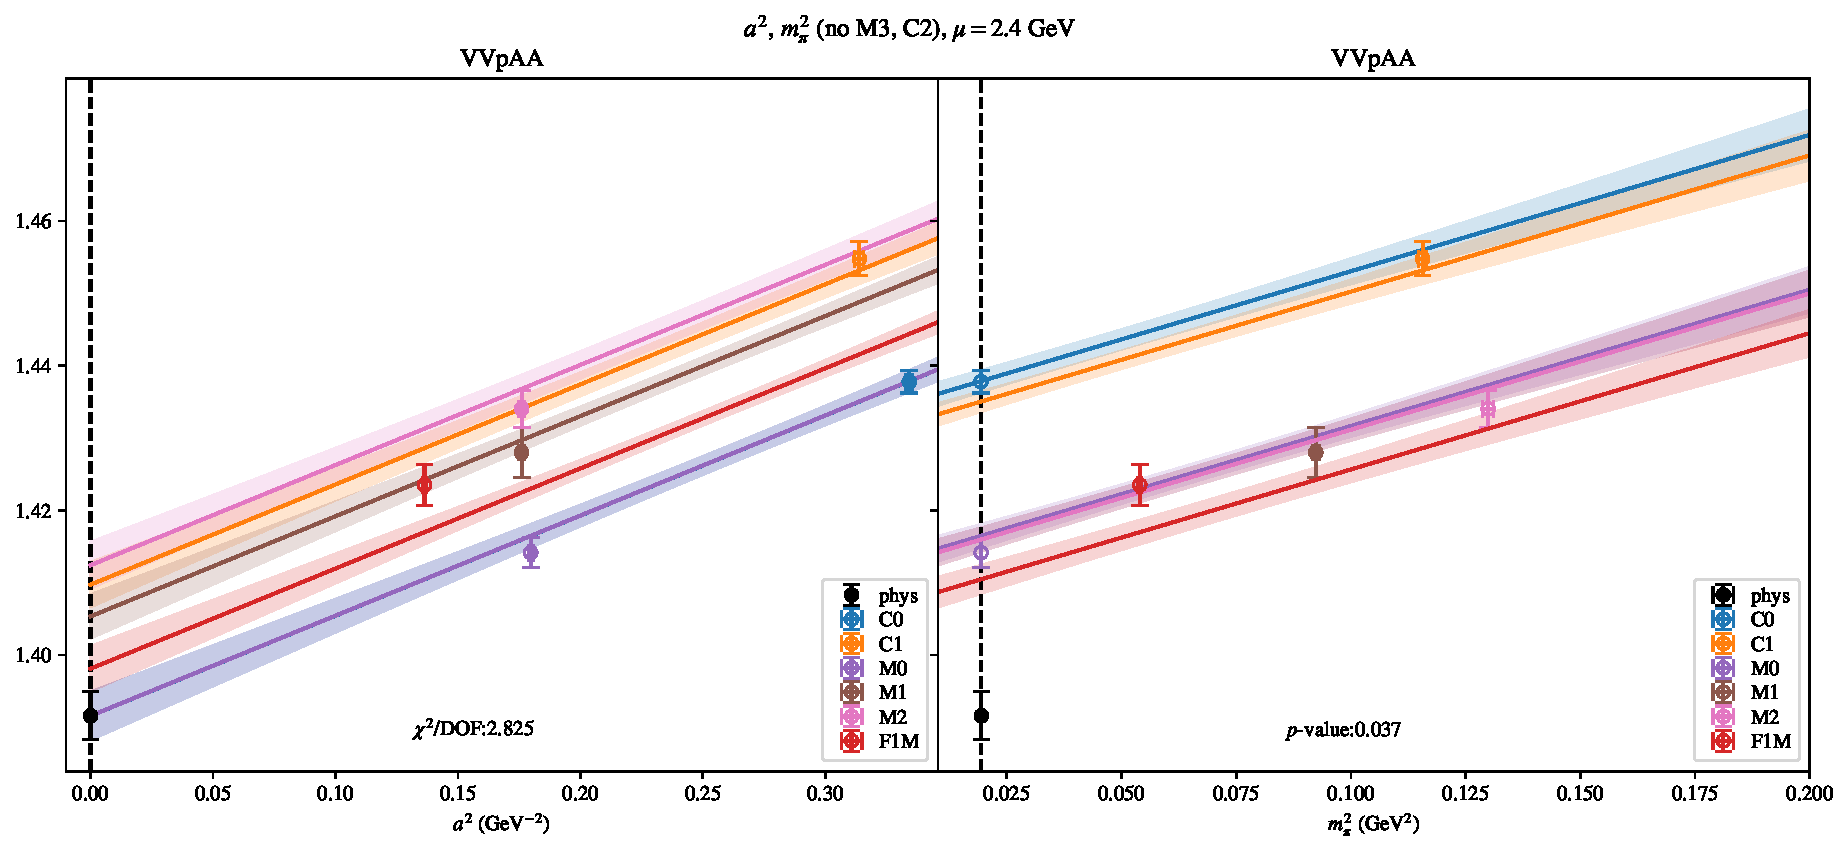
\includepdf[link, pages=-]{VVpAA/SUSY/bag_a2m2mcut_24.pdf}
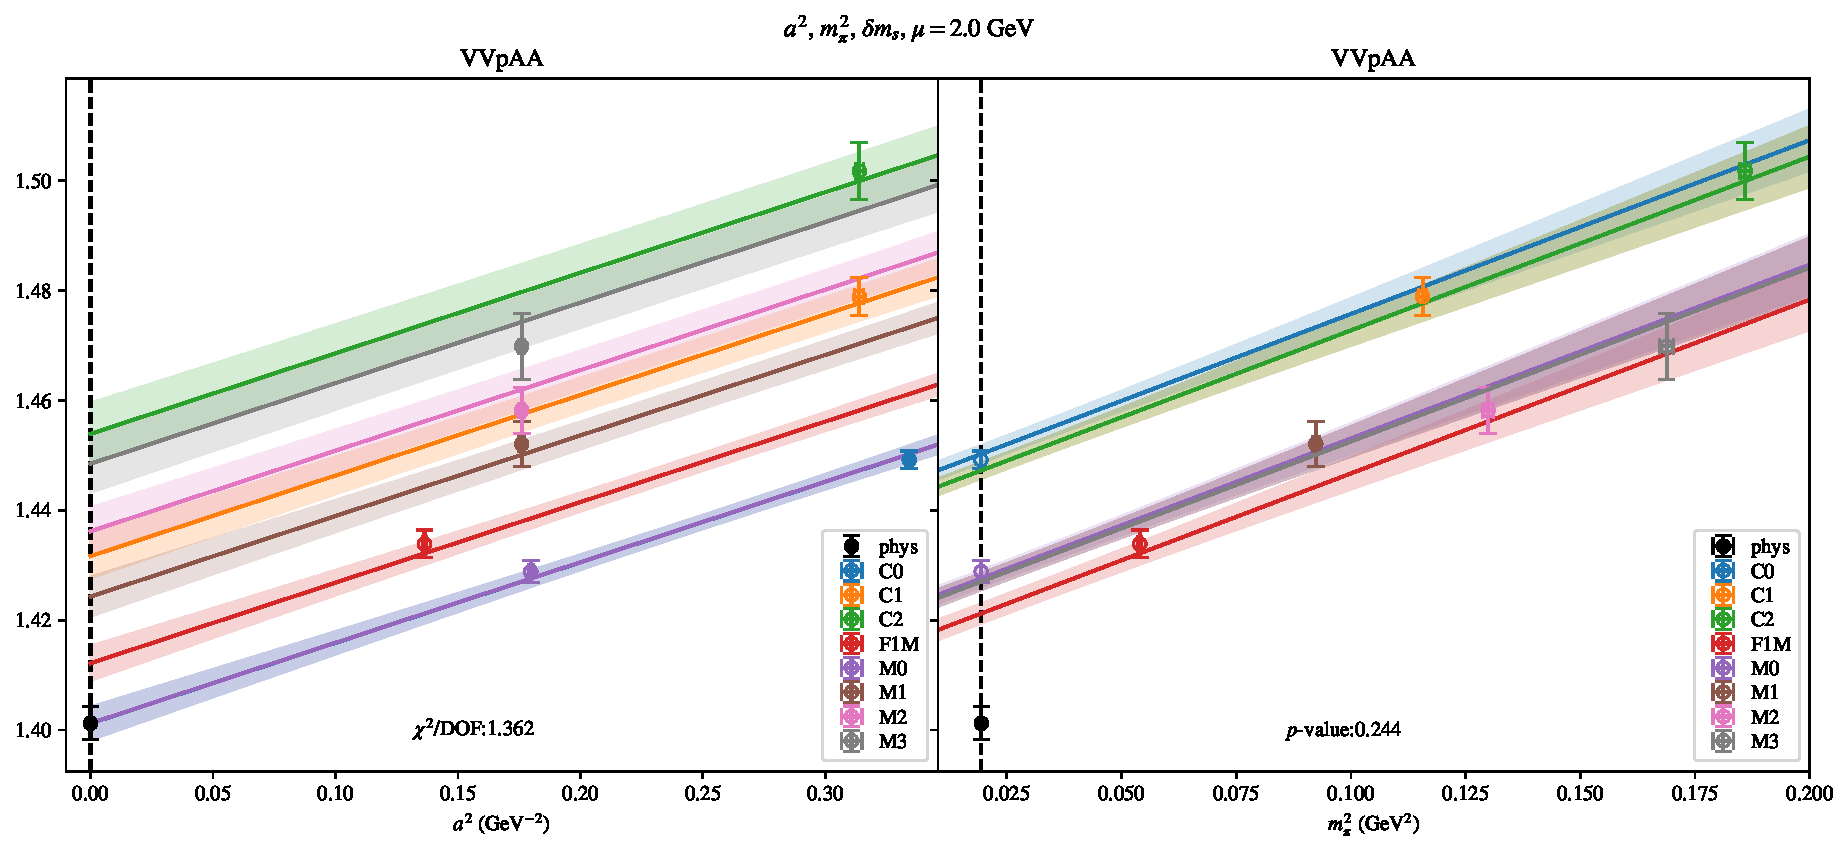
\includepdf[link, pages=-]{VVpAA/SUSY/bag_a2m2delm_20.pdf}
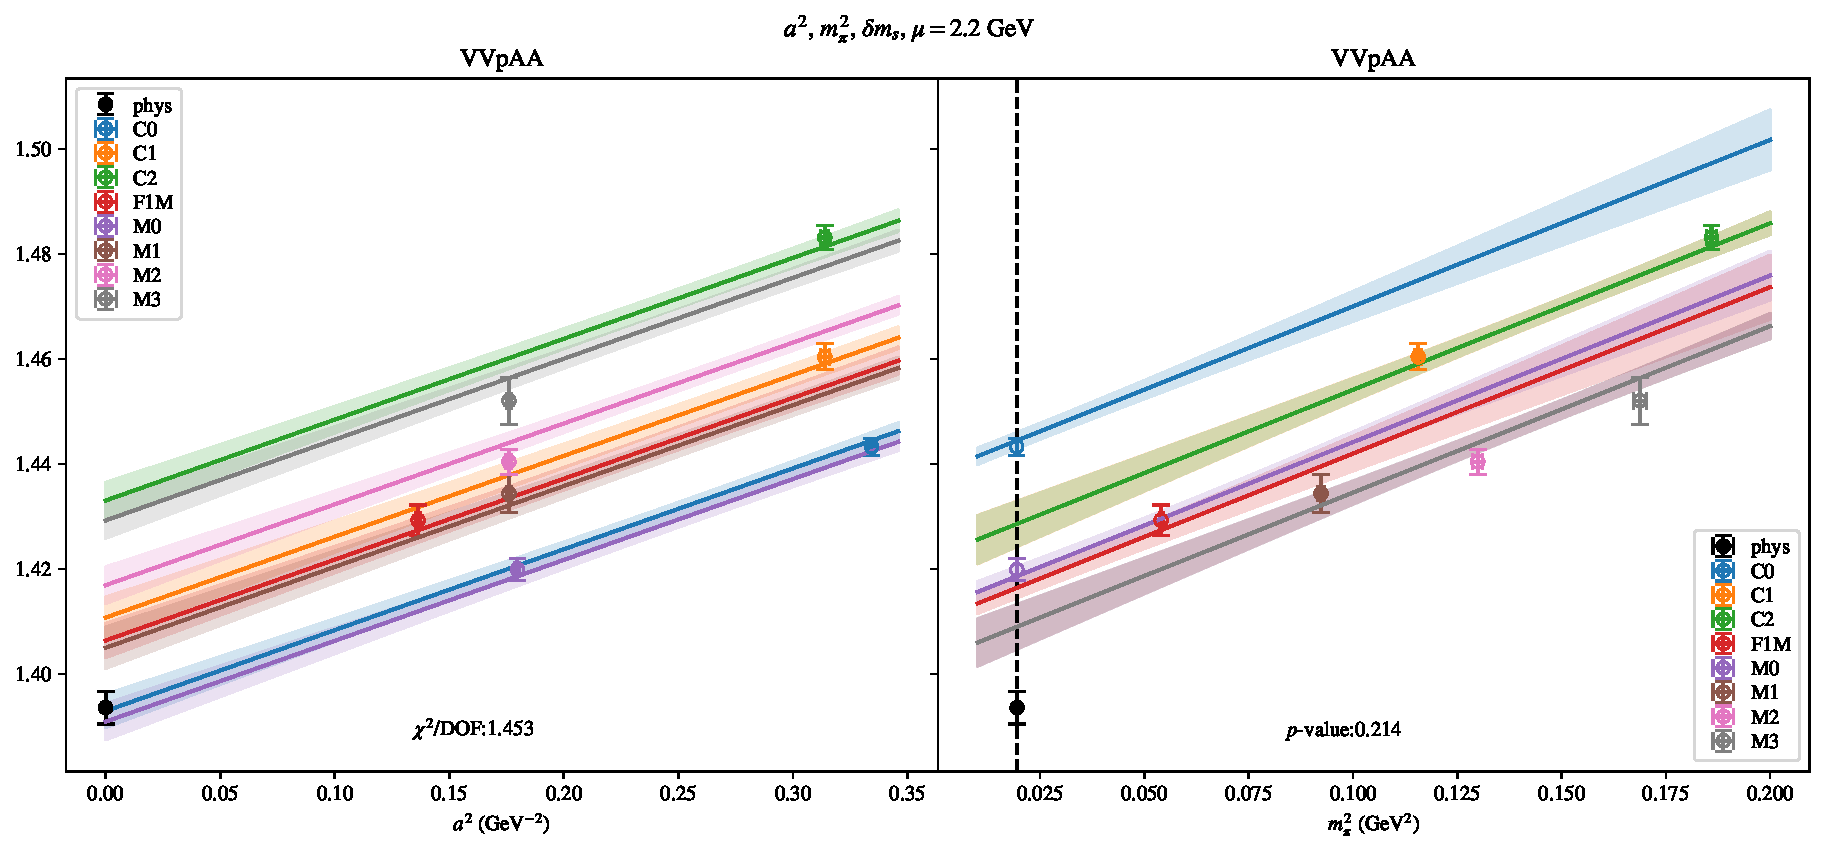
\includepdf[link, pages=-]{VVpAA/SUSY/bag_a2m2delm_22.pdf}
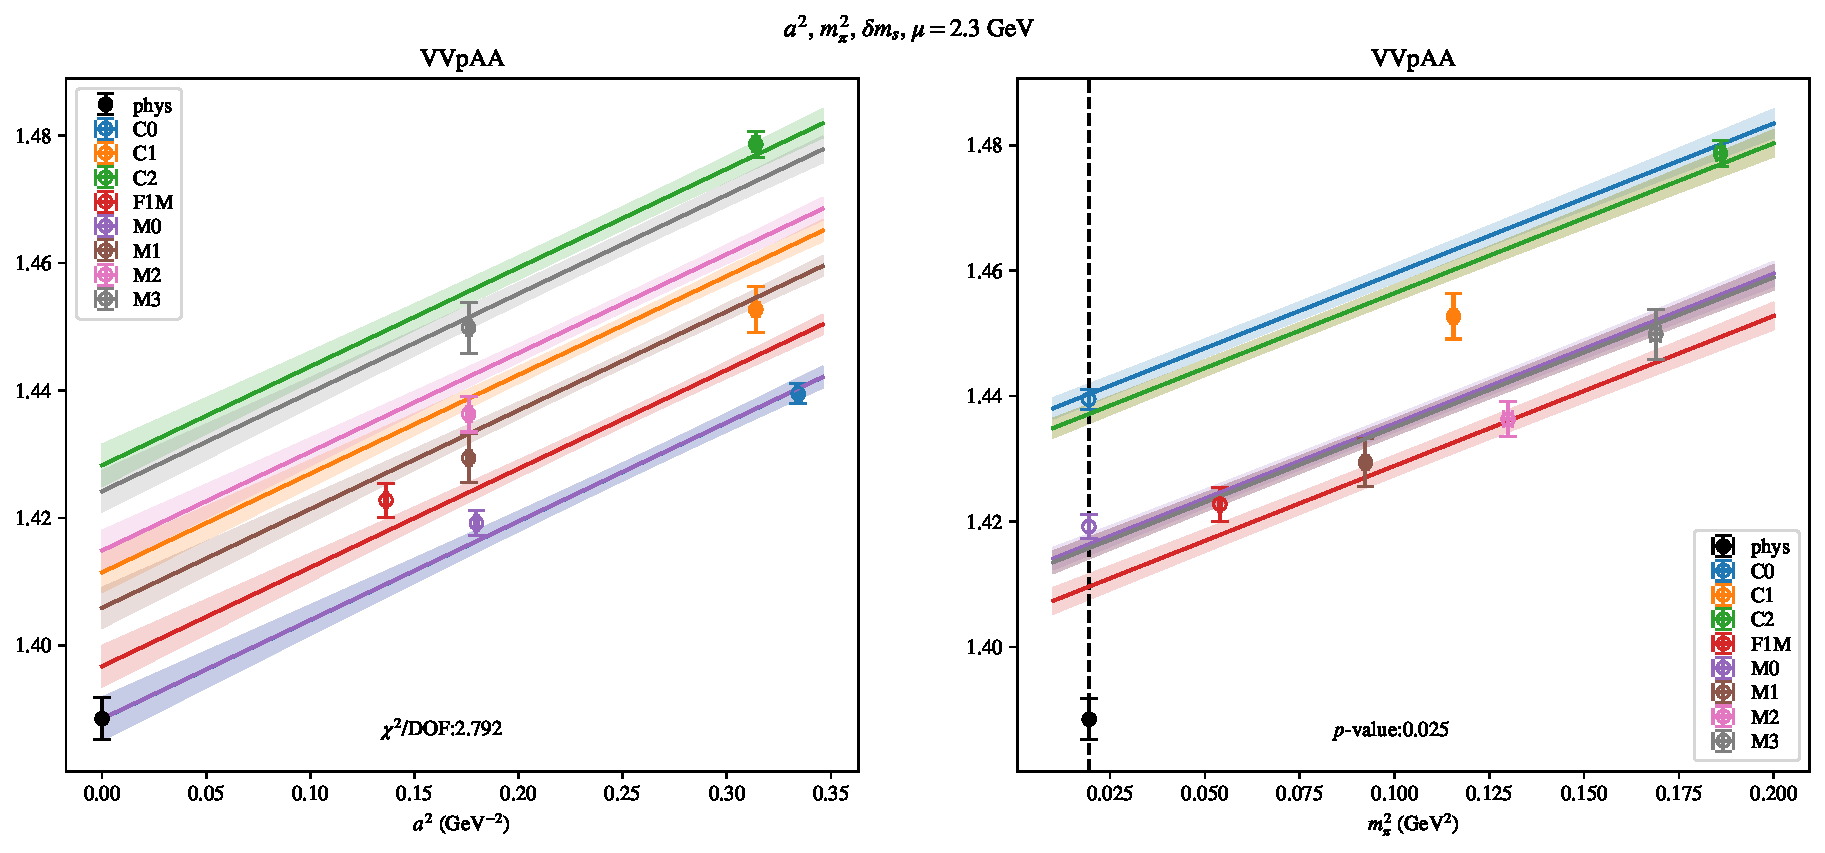
\includepdf[link, pages=-]{VVpAA/SUSY/bag_a2m2delm_23.pdf}
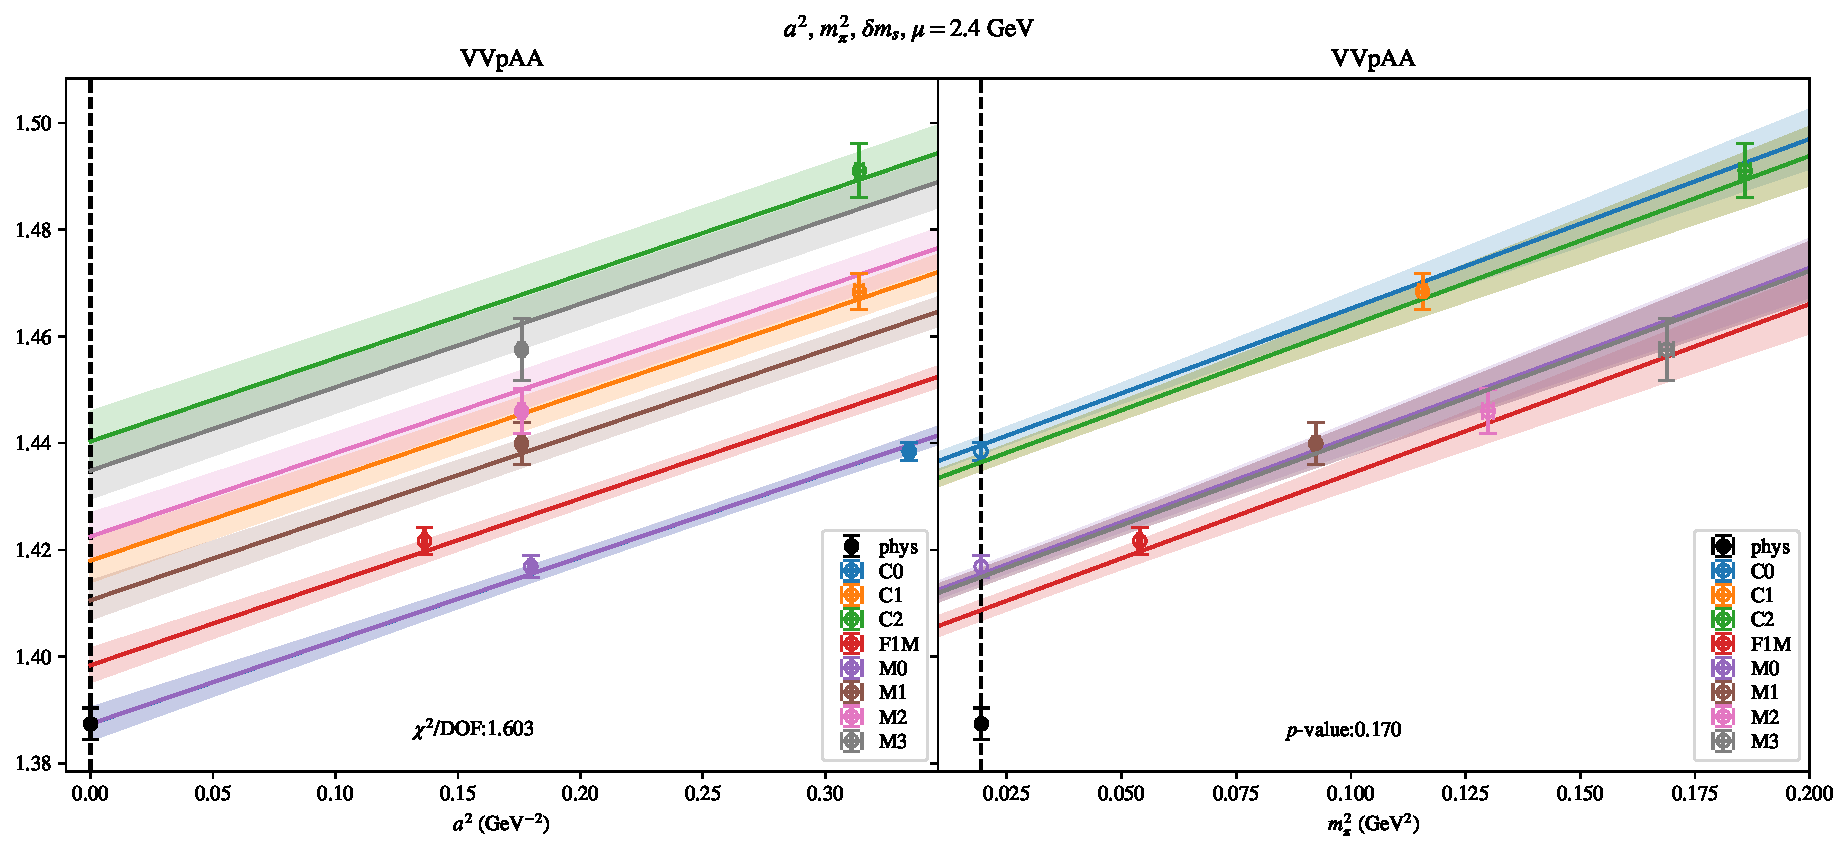
\includepdf[link, pages=-]{VVpAA/SUSY/bag_a2m2delm_24.pdf}
\clearpage
\section{$\mathcal{B}_2$}
\begin{table}[h!]
\begin{center}
\begin{tabular}{|c|c|c|c|c|c|}
\hline
$\mu$ (GeV) & $a^2$, $m_\pi^2$& $a^2$, $m_\pi^2$ (no C)& $a^2$, $m_\pi^2$, $a^4$& $a^2$, $m_\pi^2$ (no M3, C2)& $a^2$, $m_\pi^2$, $\delta m_s$\\
\hline
2.0& \hyperlink{VVmAA/SUSY/bag_a2m2_20.pdf.1}{\textbf{-0.9236(26)}: 1.129 (0.342)} & \hyperlink{VVmAA/SUSY/bag_a2m2noC_20.pdf.1}{\textbf{-0.939(11)}: 0.837 (0.433)} & \hyperlink{VVmAA/SUSY/bag_a2a4m2_20.pdf.1}{\textbf{-0.950(18)}: 0.913 (0.455)} & \hyperlink{VVmAA/SUSY/bag_a2m2mcut_20.pdf.1}{\textbf{-0.9226(27)}: 0.744 (0.526)} & \hyperlink{VVmAA/SUSY/bag_a2m2delm_20.pdf.1}{\textbf{-0.9238(26)}: 1.357 (0.246)}\\
2.2& \hyperlink{VVmAA/SUSY/bag_a2m2_22.pdf.1}{\textbf{-0.9065(23)}: 2.009 (0.074)} & \hyperlink{VVmAA/SUSY/bag_a2m2noC_22.pdf.1}{\textbf{-0.9270(94)}: 0.808 (0.446)} & \hyperlink{VVmAA/SUSY/bag_a2a4m2_22.pdf.1}{\textbf{-0.932(15)}: 1.807 (0.124)} & \hyperlink{VVmAA/SUSY/bag_a2m2mcut_22.pdf.1}{\textbf{-0.9058(24)}: 1.887 (0.129)} & \hyperlink{VVmAA/SUSY/bag_a2m2delm_22.pdf.1}{\textbf{-0.9065(23)}: 2.457 (0.043)}\\
2.3& \hyperlink{VVmAA/SUSY/bag_a2m2_23.pdf.1}{\textbf{-0.8974(22)}: 2.895 (0.013)} & \hyperlink{VVmAA/SUSY/bag_a2m2noC_23.pdf.1}{\textbf{-0.9194(88)}: 1.21 (0.298)} & \hyperlink{VVmAA/SUSY/bag_a2a4m2_23.pdf.1}{\textbf{-0.923(15)}: 2.838 (0.023)} & \hyperlink{VVmAA/SUSY/bag_a2m2mcut_23.pdf.1}{\textbf{-0.8968(23)}: 3.024 (0.028)} & \hyperlink{VVmAA/SUSY/bag_a2m2delm_23.pdf.1}{\textbf{-0.8974(22)}: 3.583 (0.006)}\\
2.4& \hyperlink{VVmAA/SUSY/bag_a2m2_24.pdf.1}{\textbf{-0.8892(22)}: 3.477 (0.004)} & \hyperlink{VVmAA/SUSY/bag_a2m2noC_24.pdf.1}{\textbf{-0.9121(86)}: 1.522 (0.218)} & \hyperlink{VVmAA/SUSY/bag_a2a4m2_24.pdf.1}{\textbf{-0.915(14)}: 3.475 (0.008)} & \hyperlink{VVmAA/SUSY/bag_a2m2mcut_24.pdf.1}{\textbf{-0.8887(23)}: 3.743 (0.011)} & \hyperlink{VVmAA/SUSY/bag_a2m2delm_24.pdf.1}{\textbf{-0.8892(21)}: 4.323 (0.002)}\\
\hline
\end{tabular}
\caption{Physical point value from chiral and continuum extrapolation at renormalisation scale $\mu$. Entries are \textbf{value(error)}: $\chi^2/\text{DOF}$ ($p$-value).}
\end{center}
\end{table}
\begin{table}[h!]
\begin{center}
\begin{tabular}{|c c|c|c|c|c|c|}
\hline
$\mu$ (GeV) &  & $a^2$, $m_\pi^2$& $a^2$, $m_\pi^2$ (no C)& $a^2$, $m_\pi^2$, $a^4$& $a^2$, $m_\pi^2$ (no M3, C2)& $a^2$, $m_\pi^2$, $\delta m_s$\\
\hline
\multirow{3}{0.5in}{2.0} & $\alpha$ & -0.360(10)& -0.269(67)& -0.12(16)& -0.363(11)& -0.360(10)\\
 & $\beta$ & -0.00711(29)& -0.00721(54)& -0.00716(29)& -0.00783(49)& -0.00732(49)\\
 & $\gamma$ &  &  & -0.47(33)&  & 0.009(16)\\
\hline
\multirow{3}{0.5in}{2.2} & $\alpha$ & -0.3831(85)& -0.263(54)& -0.15(14)& -0.3849(88)& -0.3836(84)\\
 & $\beta$ & -0.00680(20)& -0.00651(39)& -0.00689(21)& -0.00734(35)& -0.00697(39)\\
 & $\gamma$ &  &  & -0.47(29)&  & 0.007(13)\\
\hline
\multirow{3}{0.5in}{2.3} & $\alpha$ & -0.3998(84)& -0.273(51)& -0.17(14)& -0.4011(88)& -0.4002(83)\\
 & $\beta$ & -0.00688(18)& -0.00650(34)& -0.00698(19)& -0.00737(30)& -0.00701(37)\\
 & $\gamma$ &  &  & -0.47(28)&  & 0.005(13)\\
\hline
\multirow{3}{0.5in}{2.4} & $\alpha$ & -0.4153(83)& -0.283(49)& -0.18(13)& -0.4162(87)& -0.4156(83)\\
 & $\beta$ & -0.00686(17)& -0.00648(32)& -0.00696(18)& -0.00734(29)& -0.00696(35)\\
 & $\gamma$ &  &  & -0.48(27)&  & 0.004(12)\\
\hline
\end{tabular}
\caption{Fit values of coefficients in $Q = Q_{phys} + \mathbf{\alpha} a^2 + \mathbf{\beta}\left(\frac{m_\pi^2}{f_\pi^2}-\frac{m_{\pi,PDG}^2}{f_\pi^2}\right) + \gamma(\ldots)$}
\end{center}
\end{table}
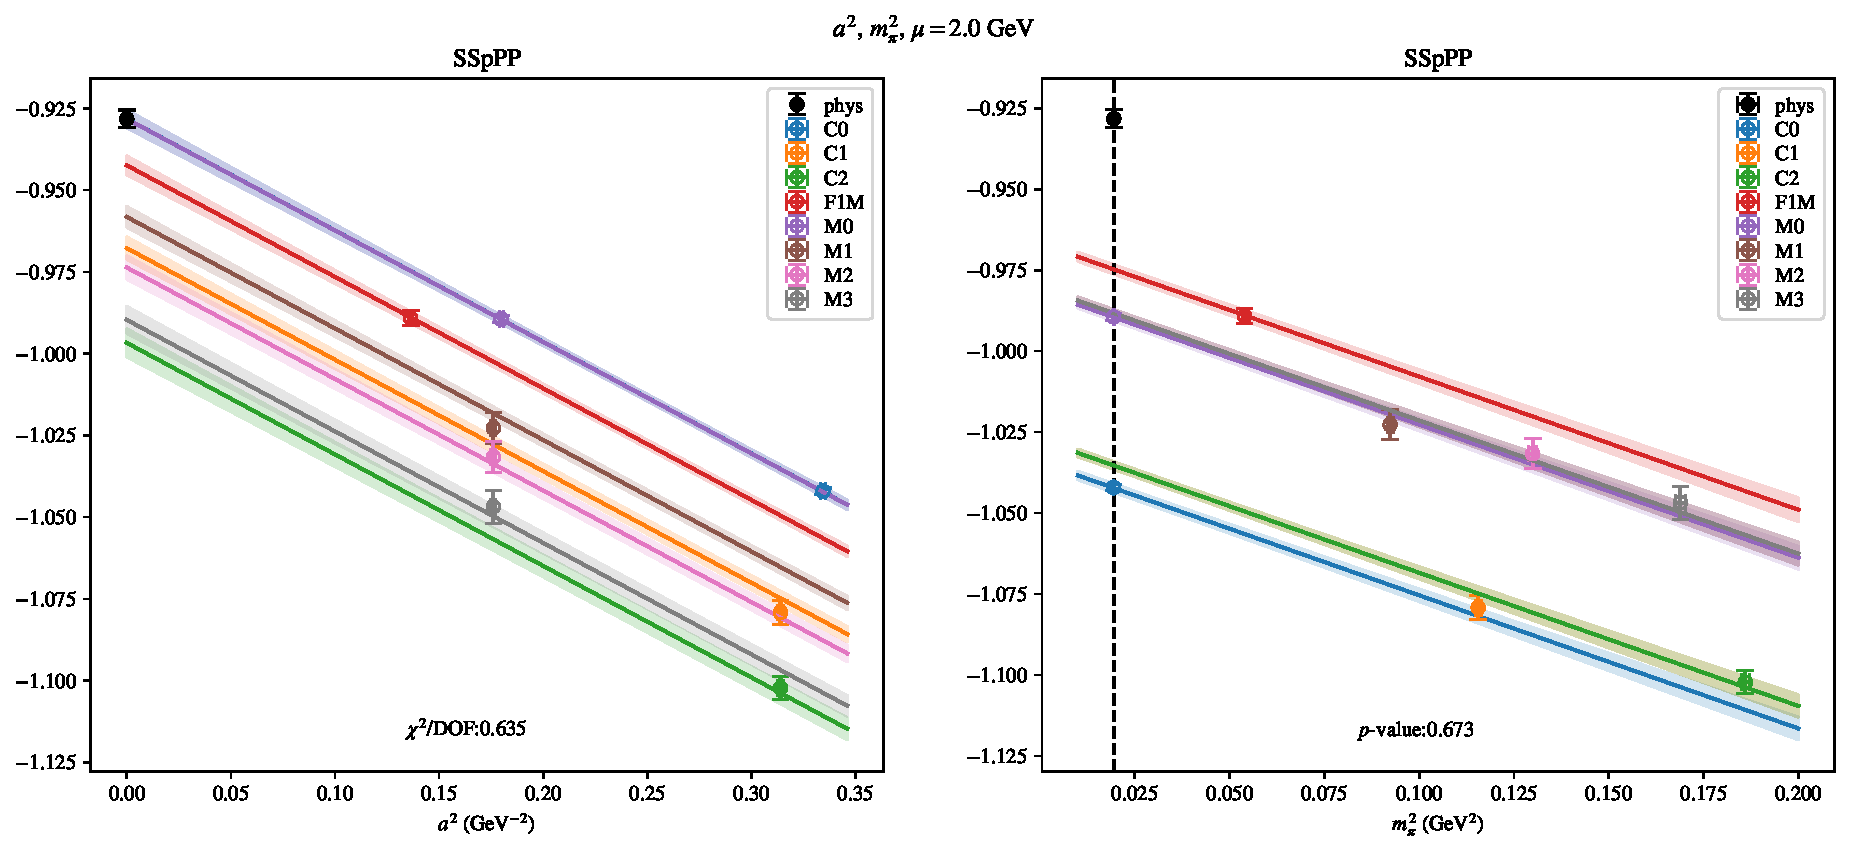
\includepdf[link, pages=-]{VVmAA/SUSY/bag_a2m2_20.pdf}
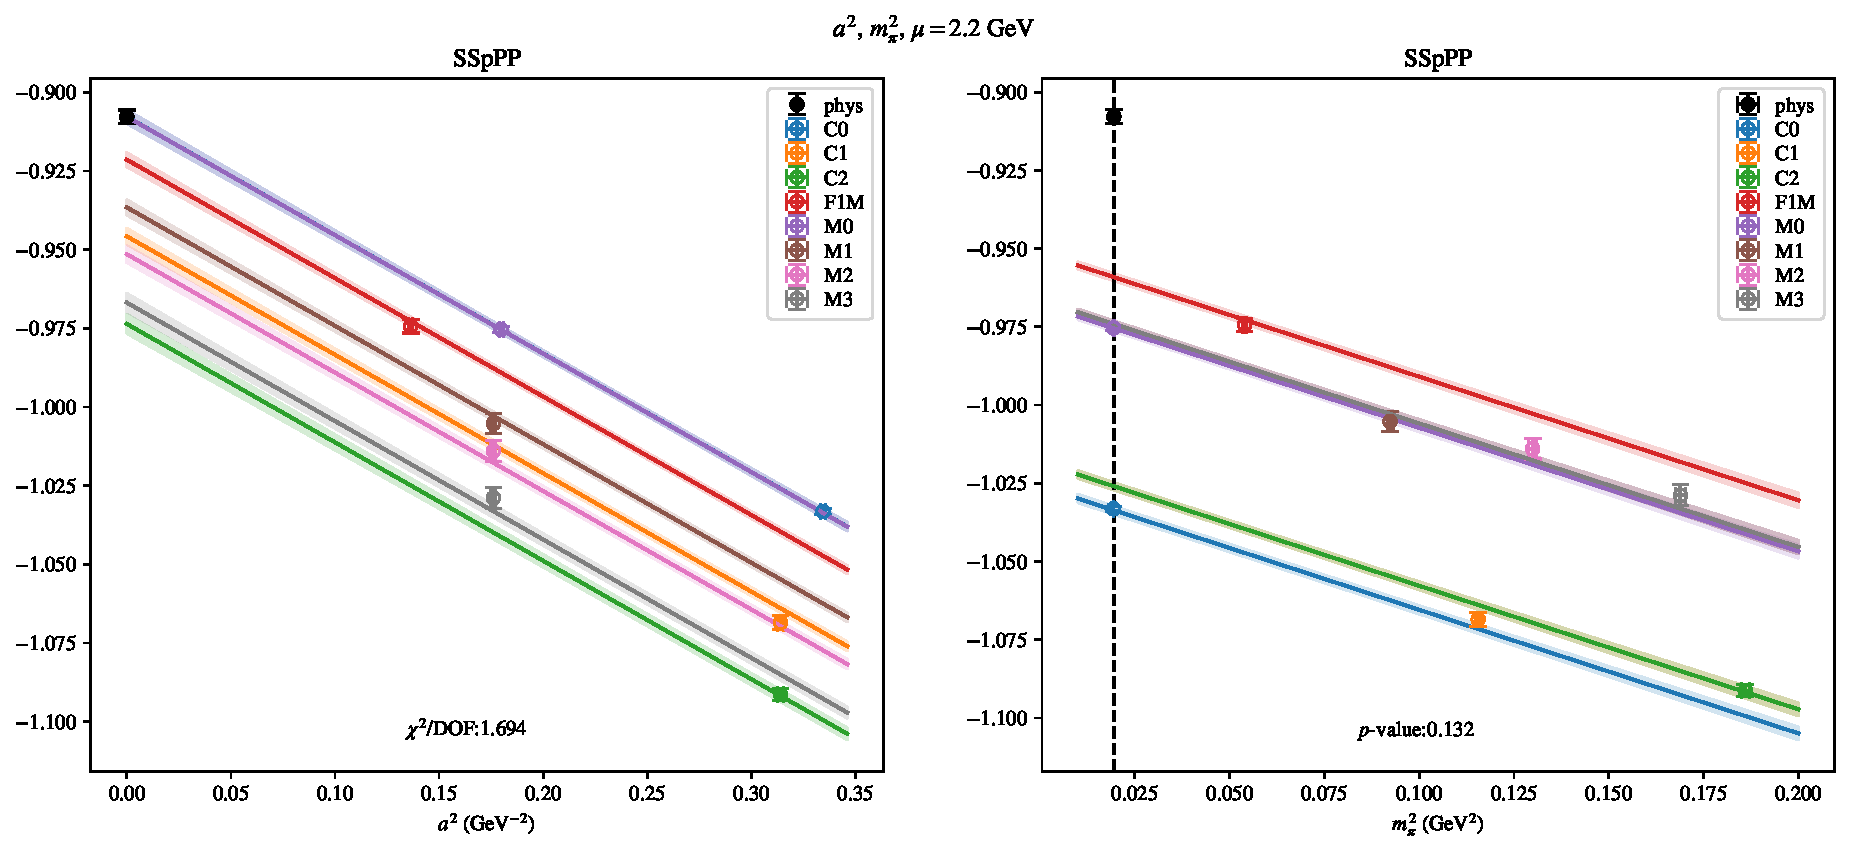
\includepdf[link, pages=-]{VVmAA/SUSY/bag_a2m2_22.pdf}
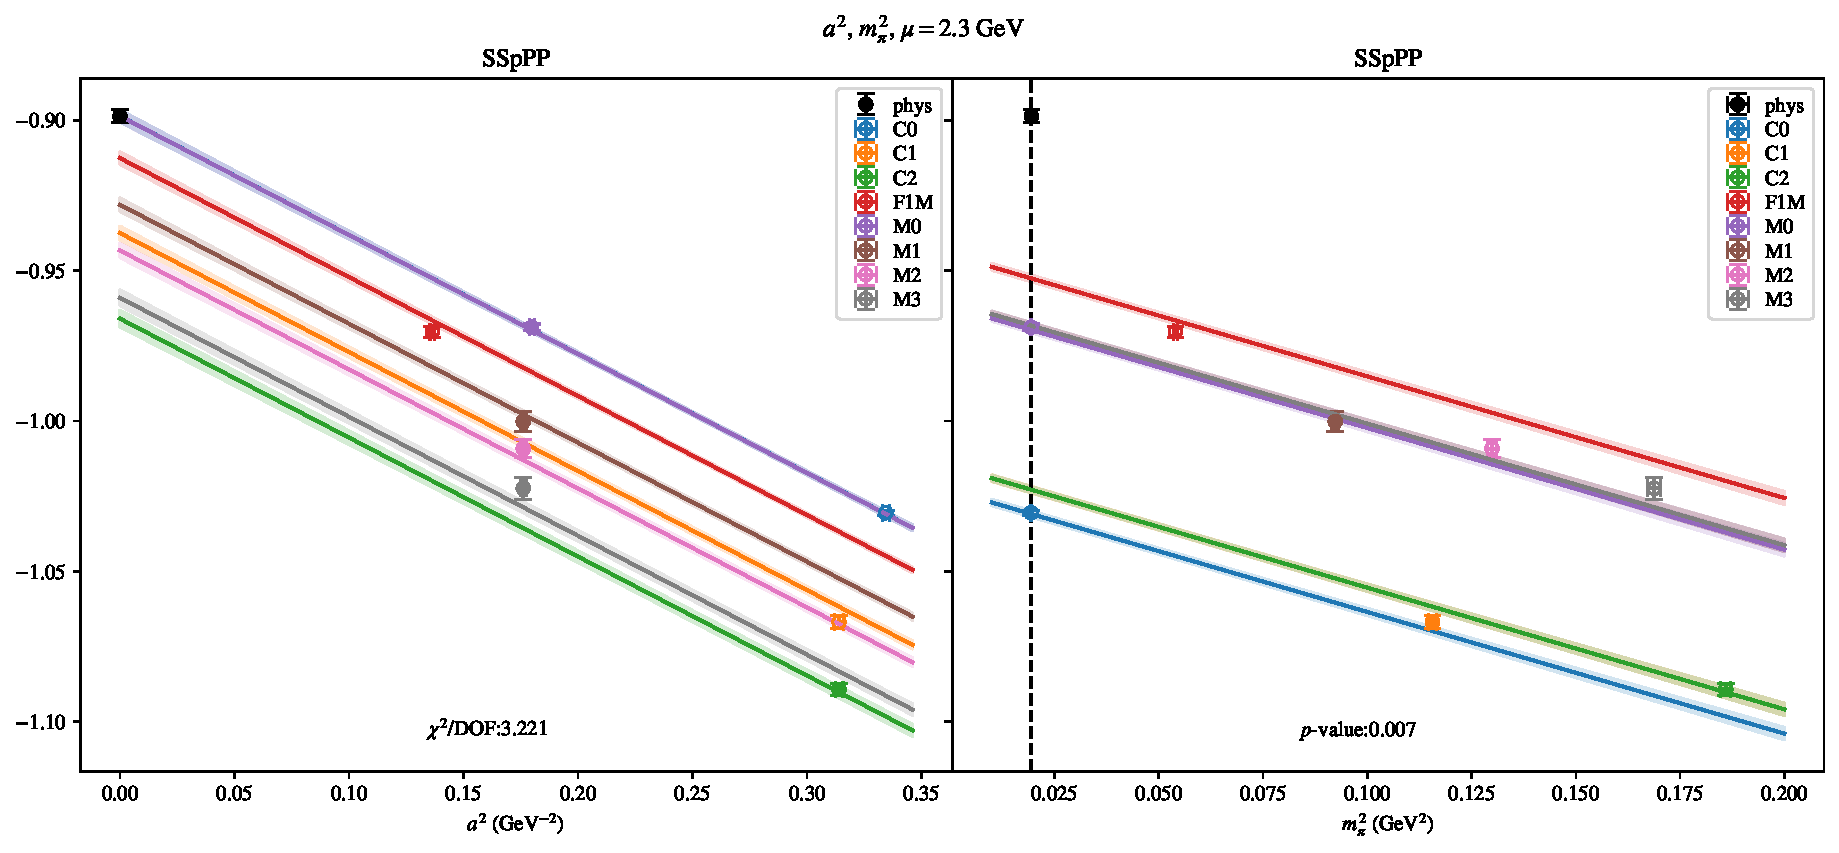
\includepdf[link, pages=-]{VVmAA/SUSY/bag_a2m2_23.pdf}
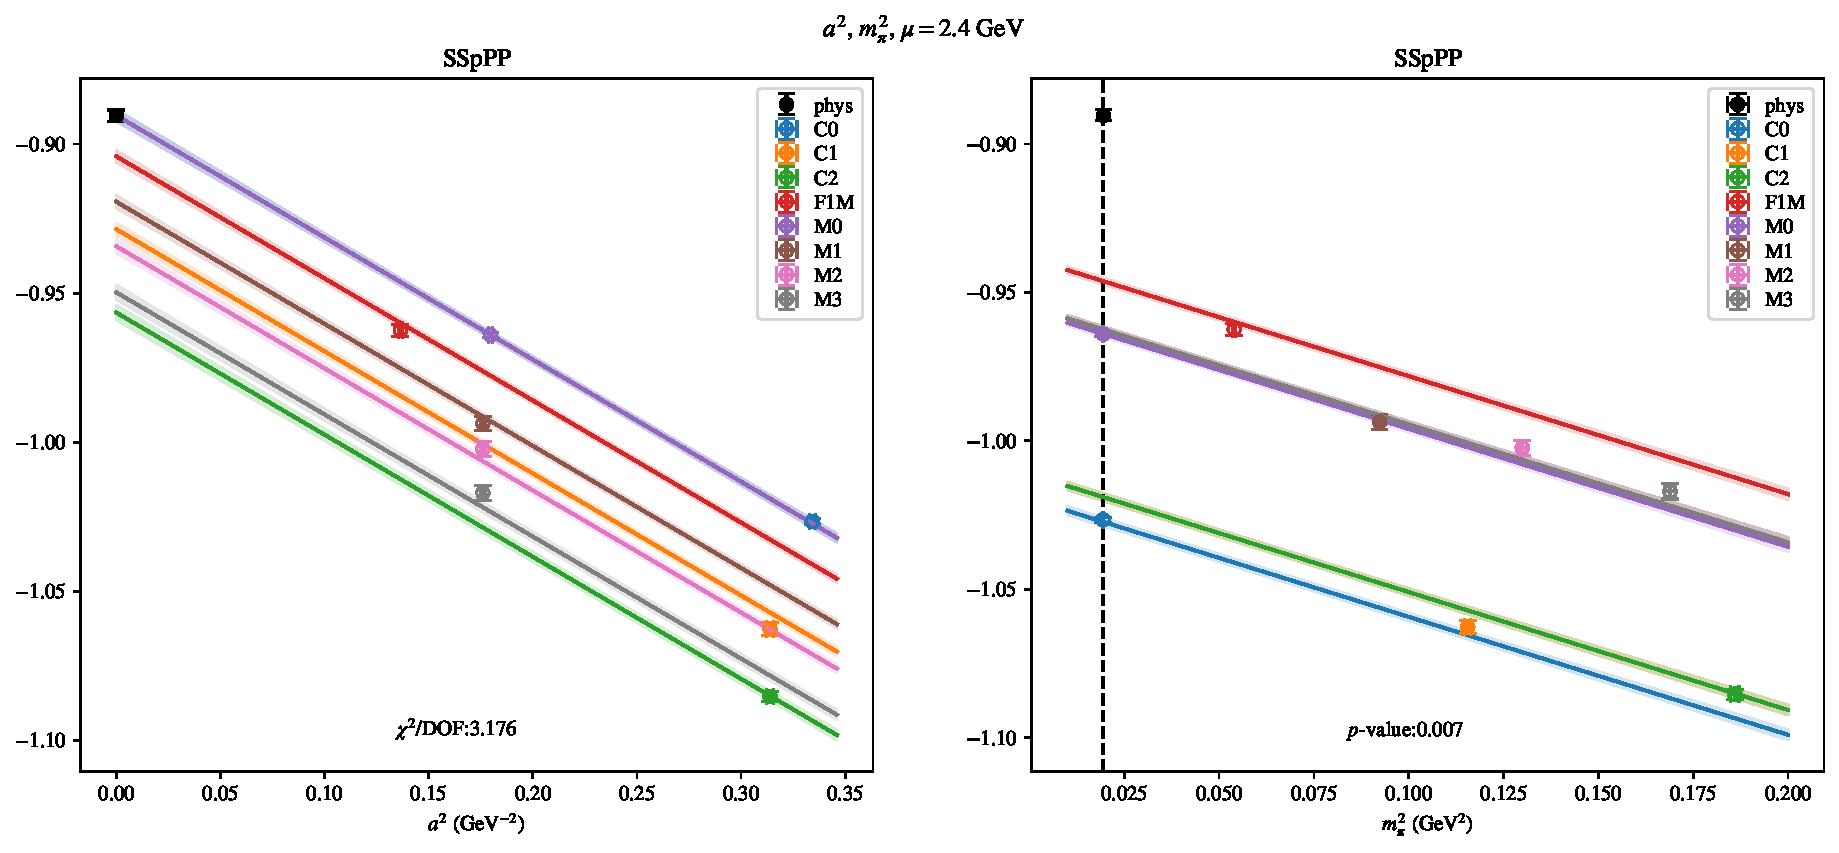
\includepdf[link, pages=-]{VVmAA/SUSY/bag_a2m2_24.pdf}
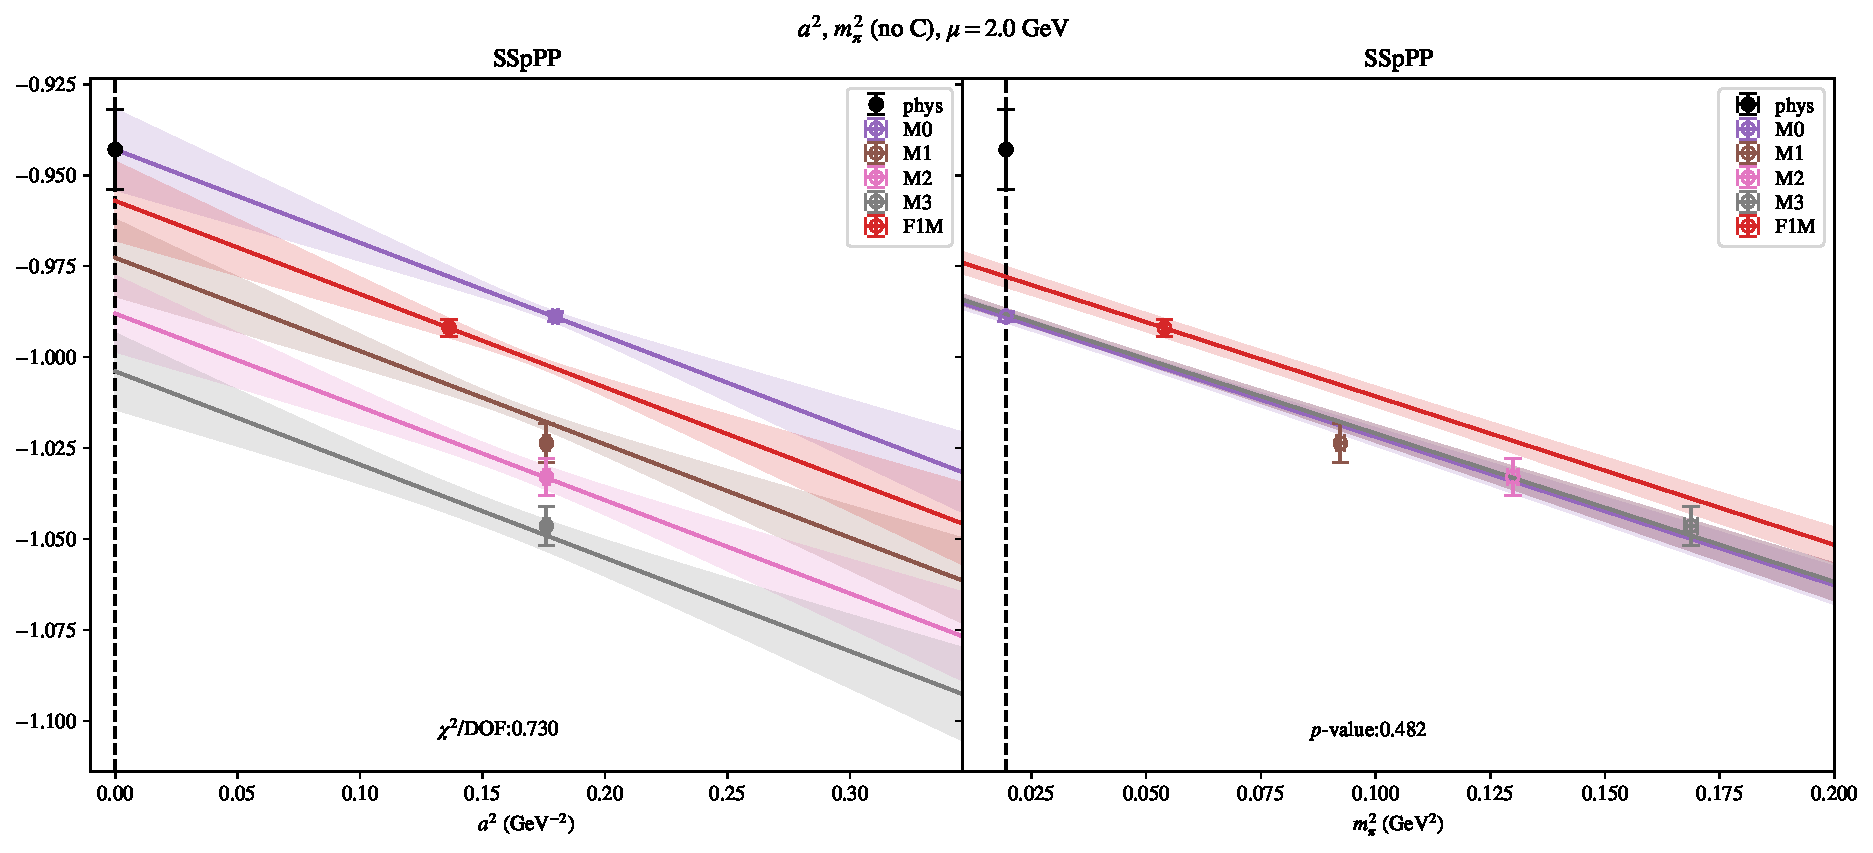
\includepdf[link, pages=-]{VVmAA/SUSY/bag_a2m2noC_20.pdf}
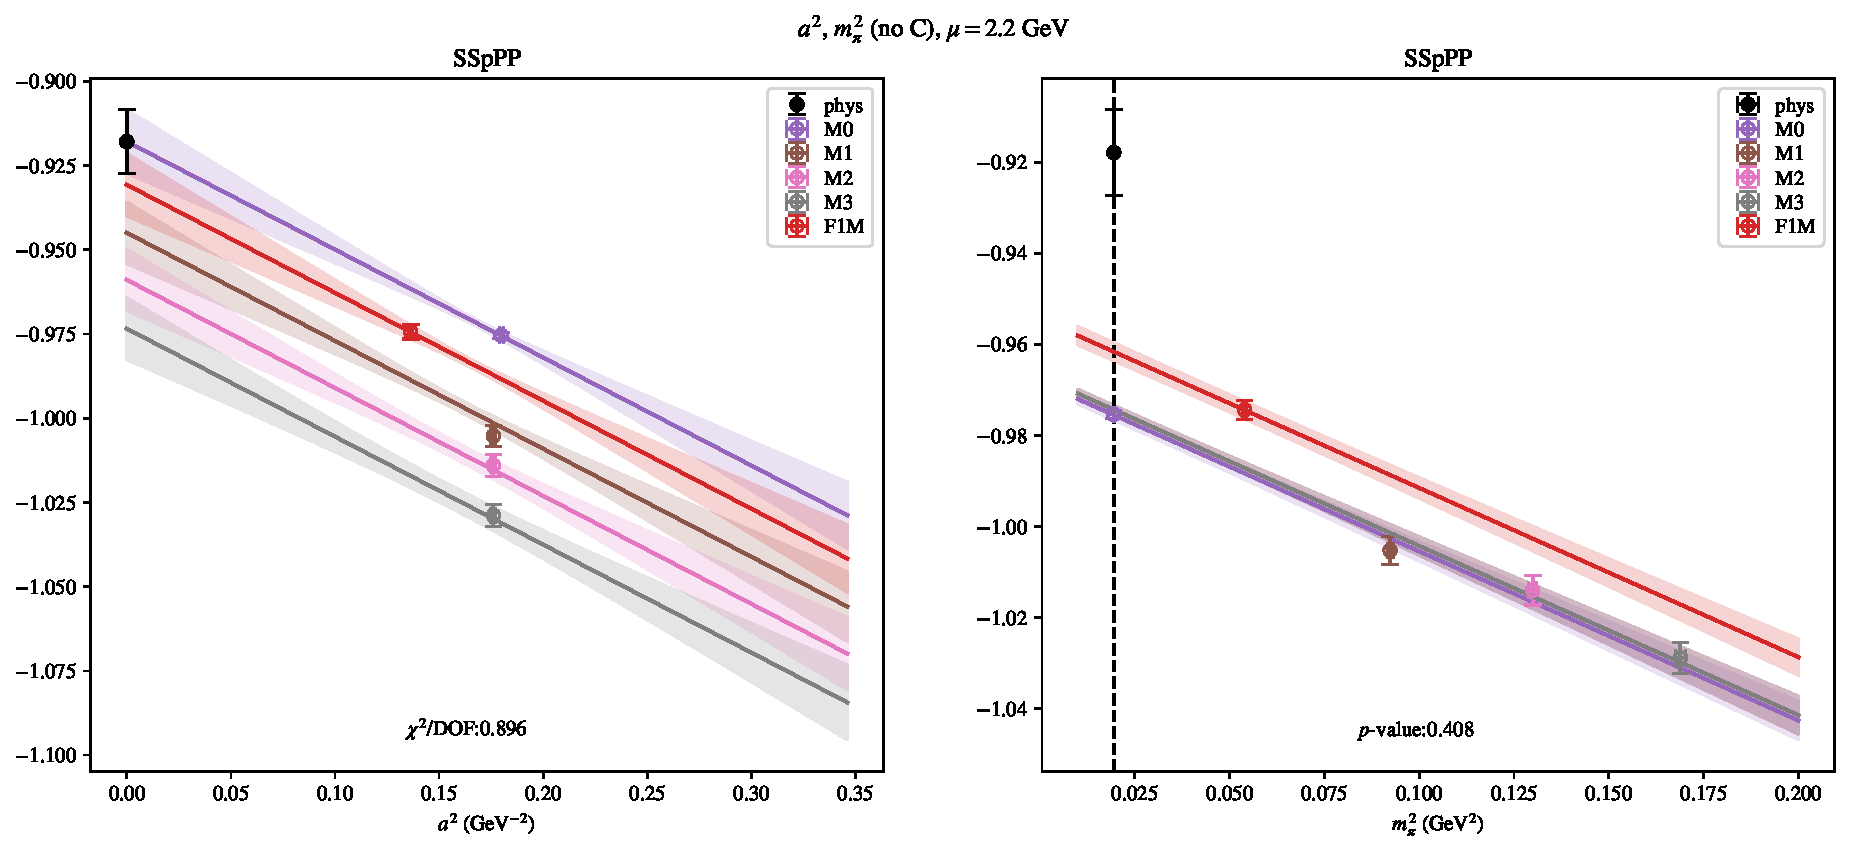
\includepdf[link, pages=-]{VVmAA/SUSY/bag_a2m2noC_22.pdf}
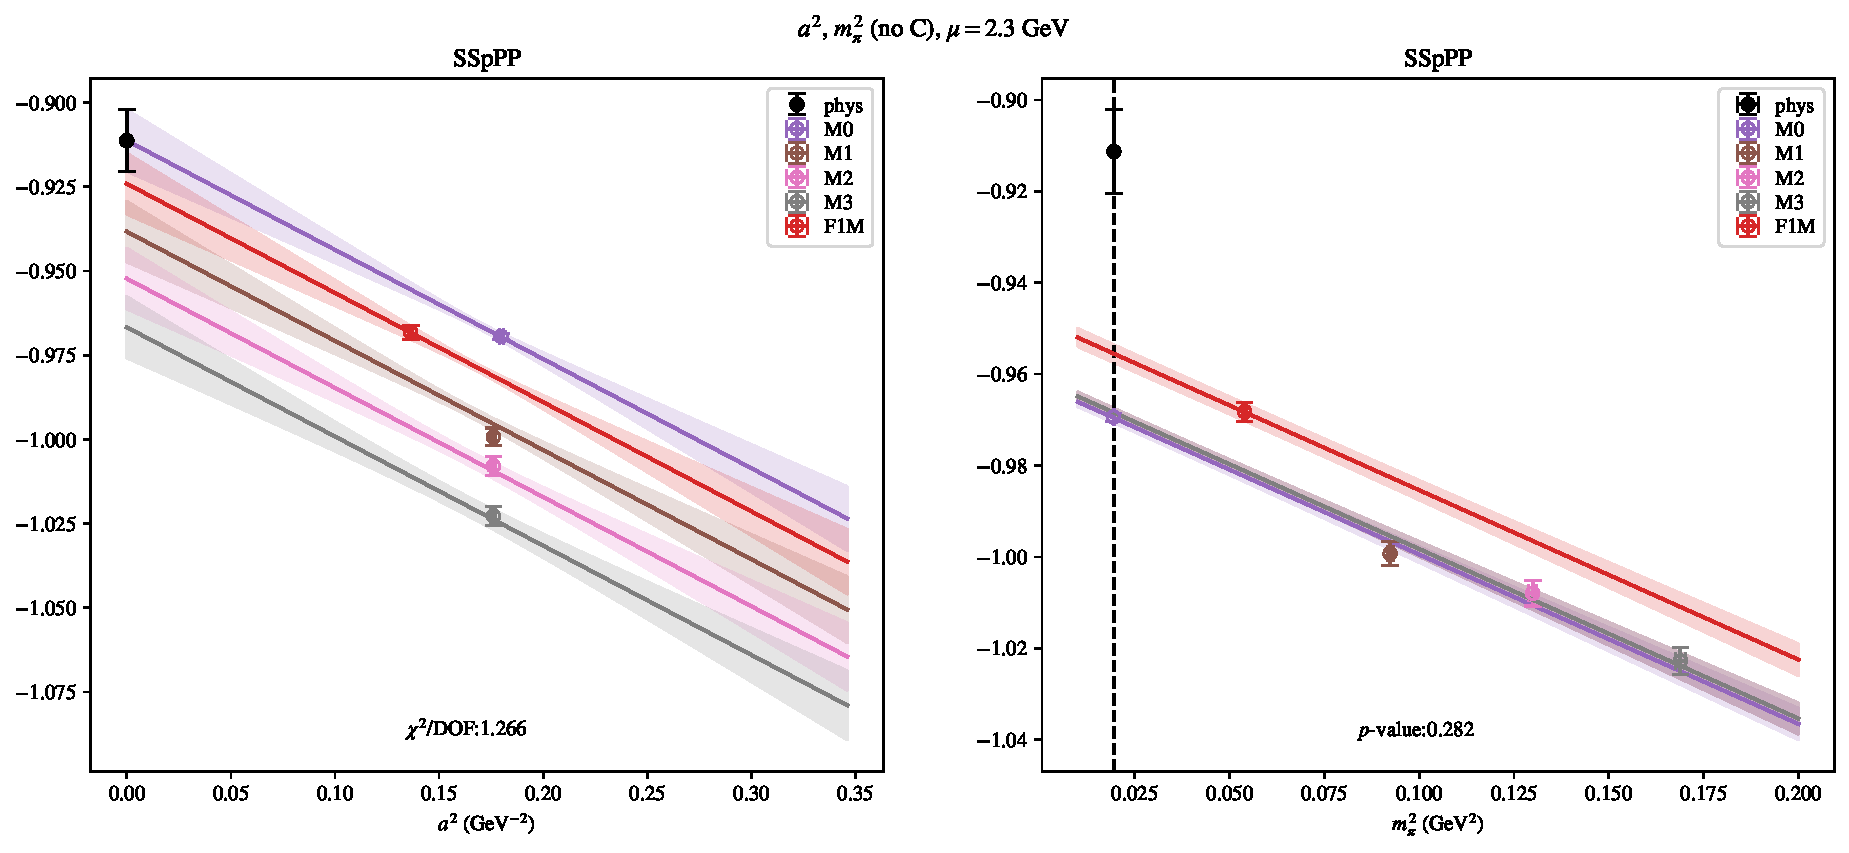
\includepdf[link, pages=-]{VVmAA/SUSY/bag_a2m2noC_23.pdf}
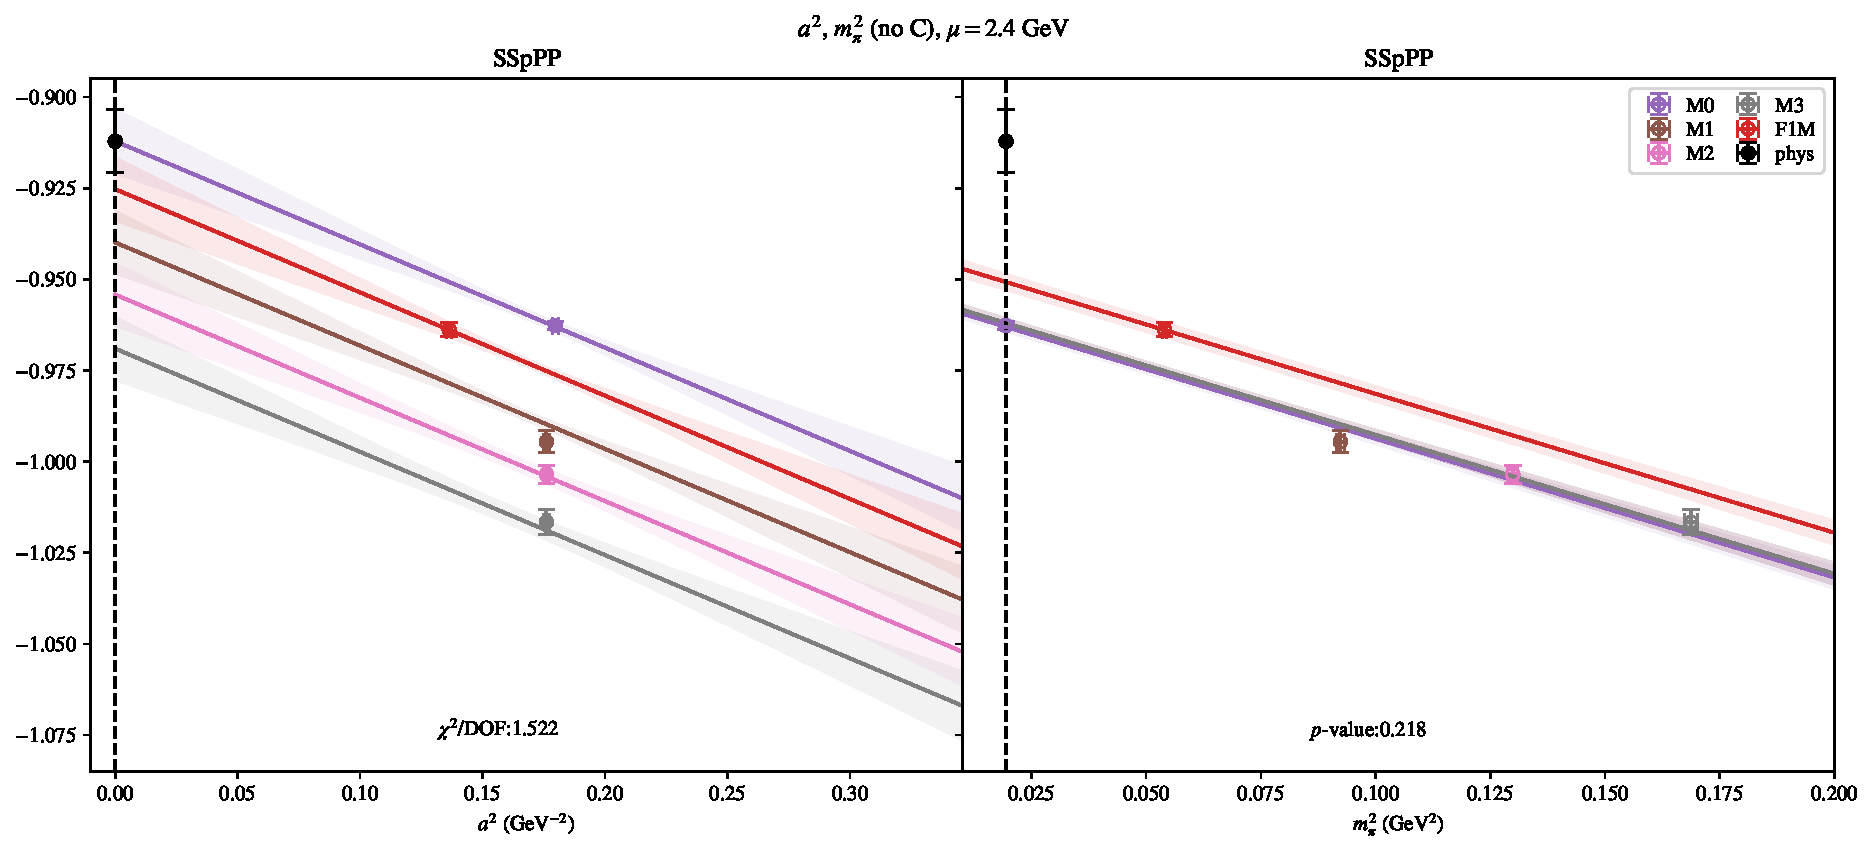
\includepdf[link, pages=-]{VVmAA/SUSY/bag_a2m2noC_24.pdf}
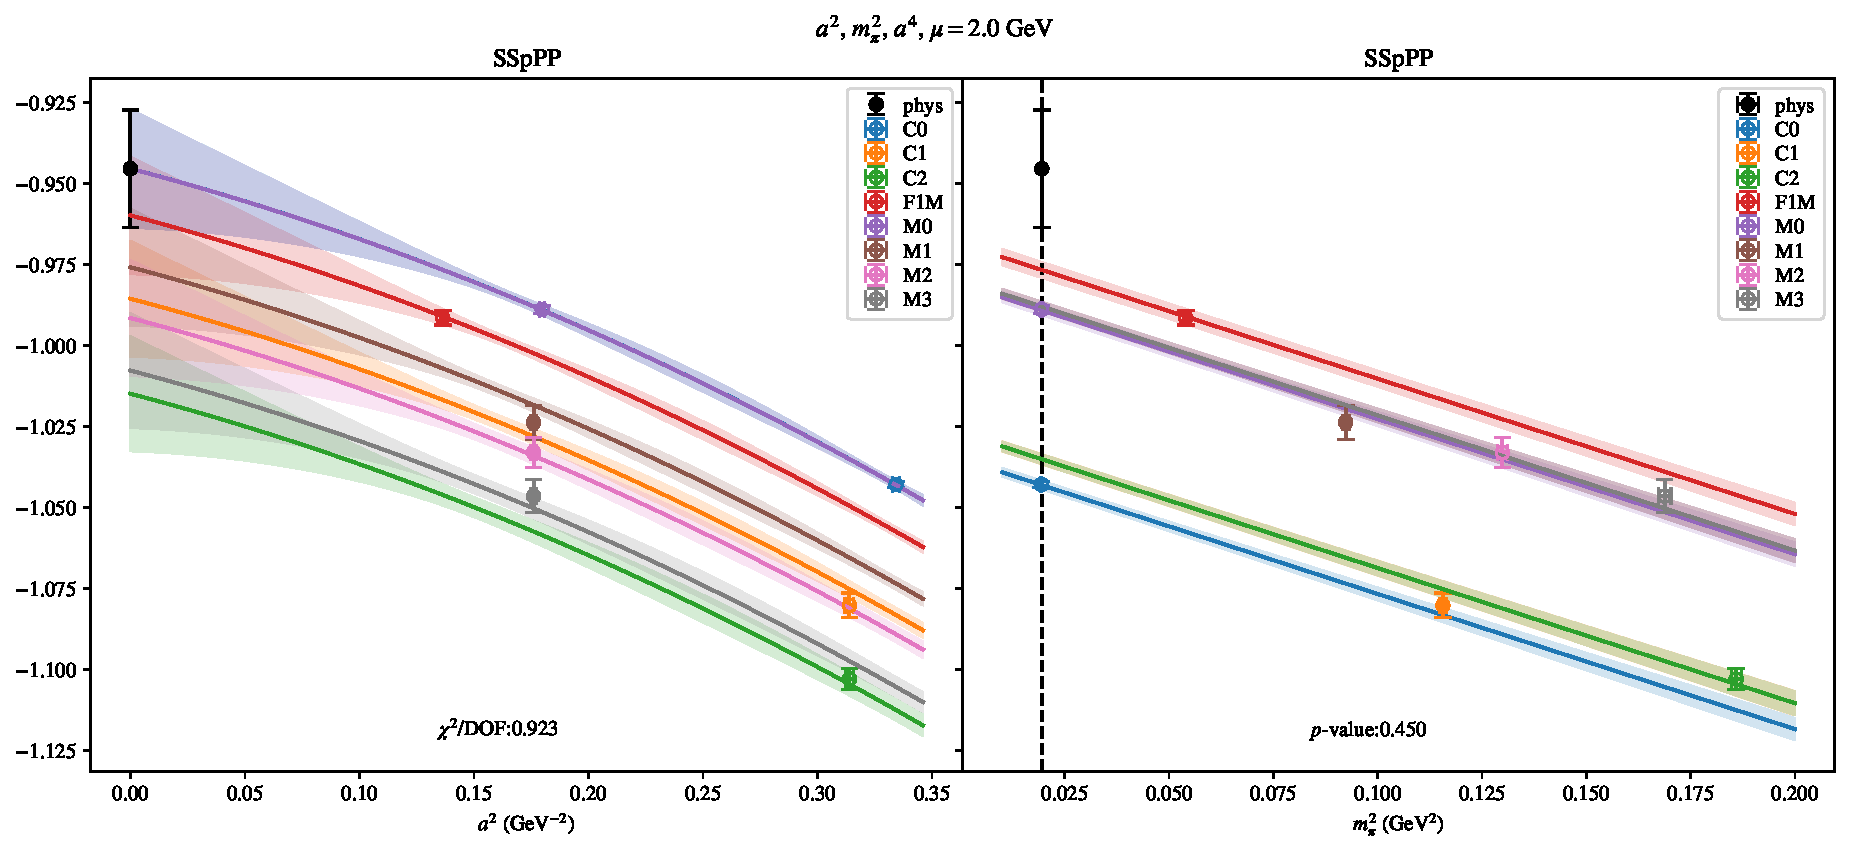
\includepdf[link, pages=-]{VVmAA/SUSY/bag_a2a4m2_20.pdf}
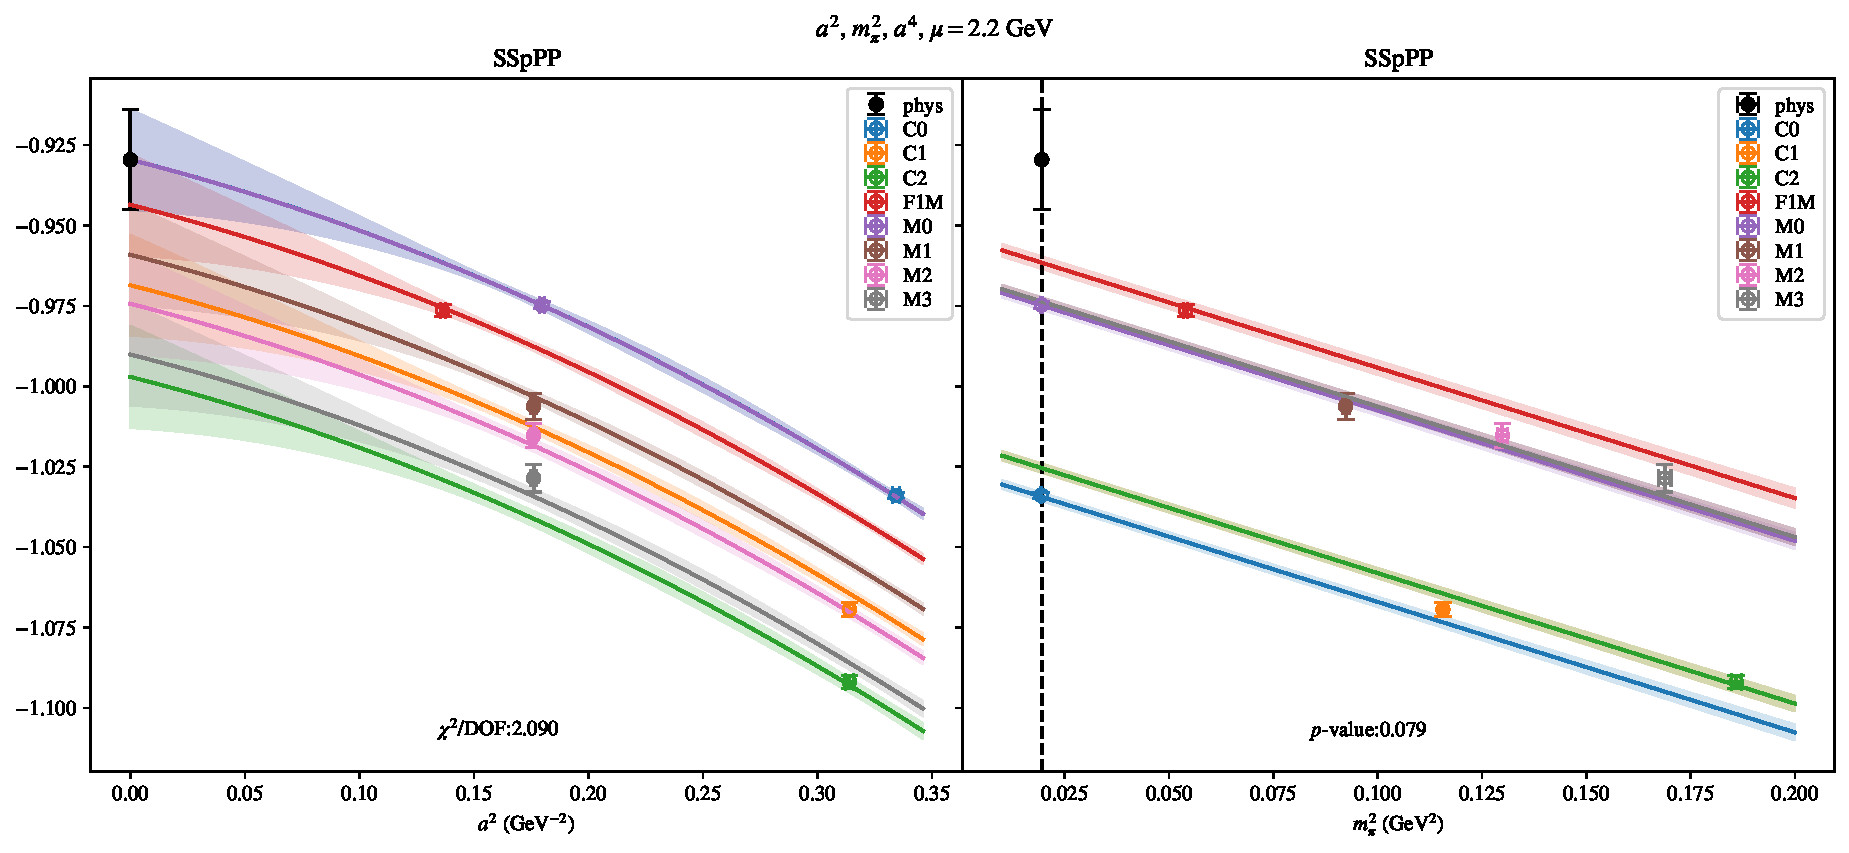
\includepdf[link, pages=-]{VVmAA/SUSY/bag_a2a4m2_22.pdf}
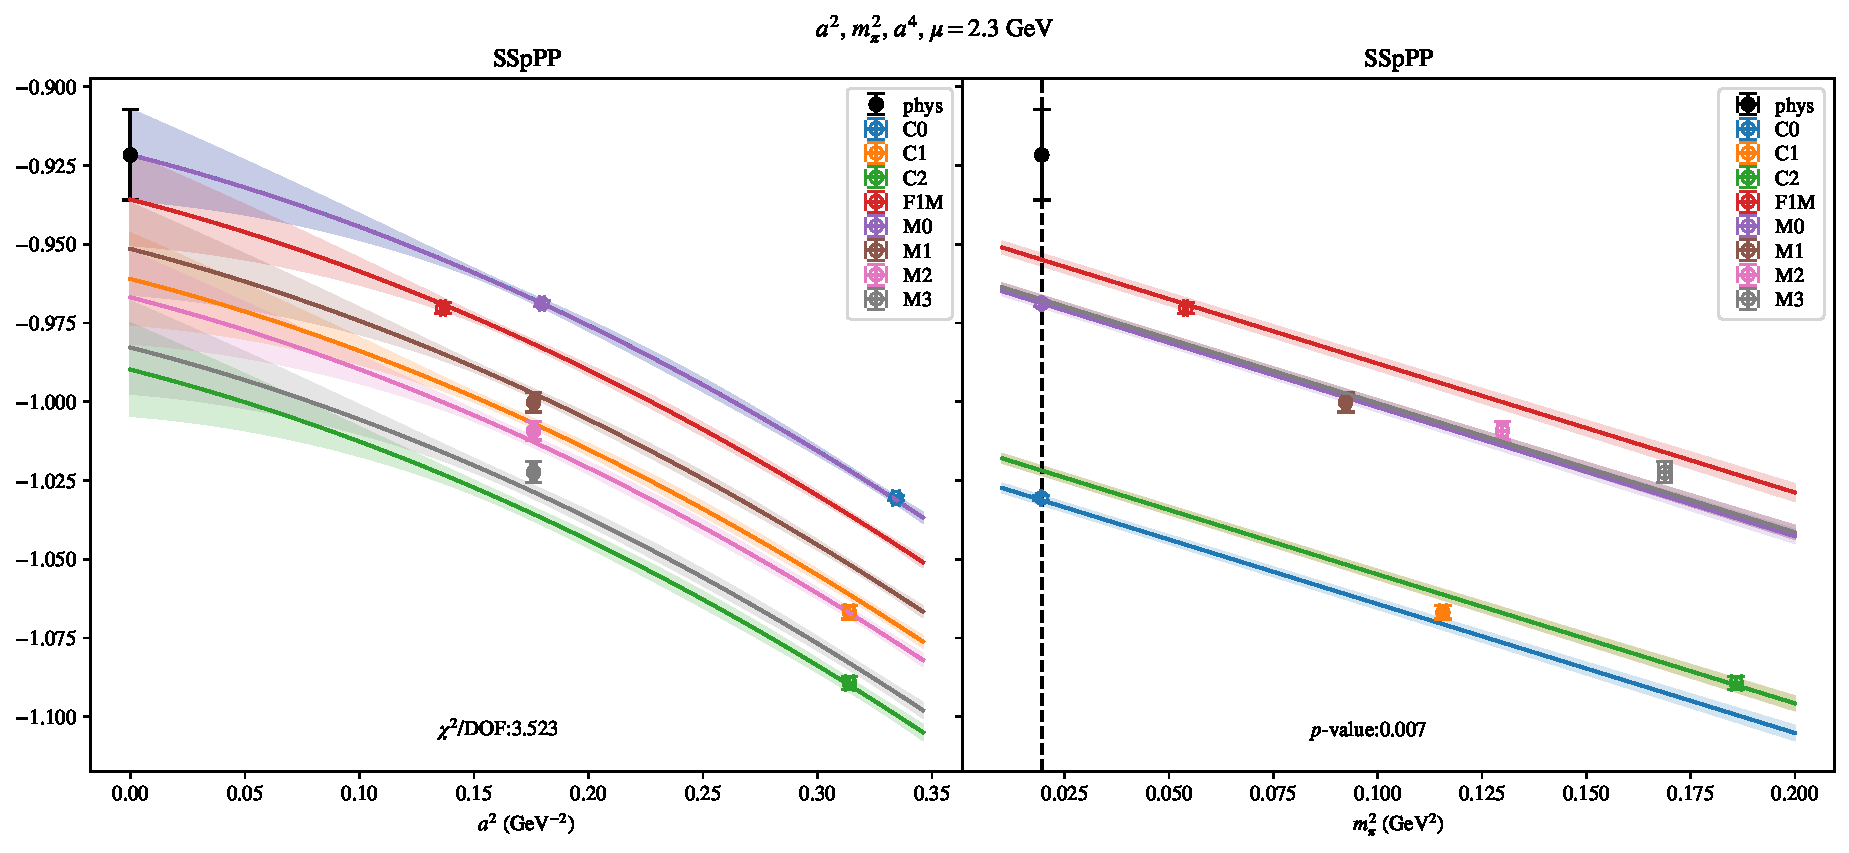
\includepdf[link, pages=-]{VVmAA/SUSY/bag_a2a4m2_23.pdf}
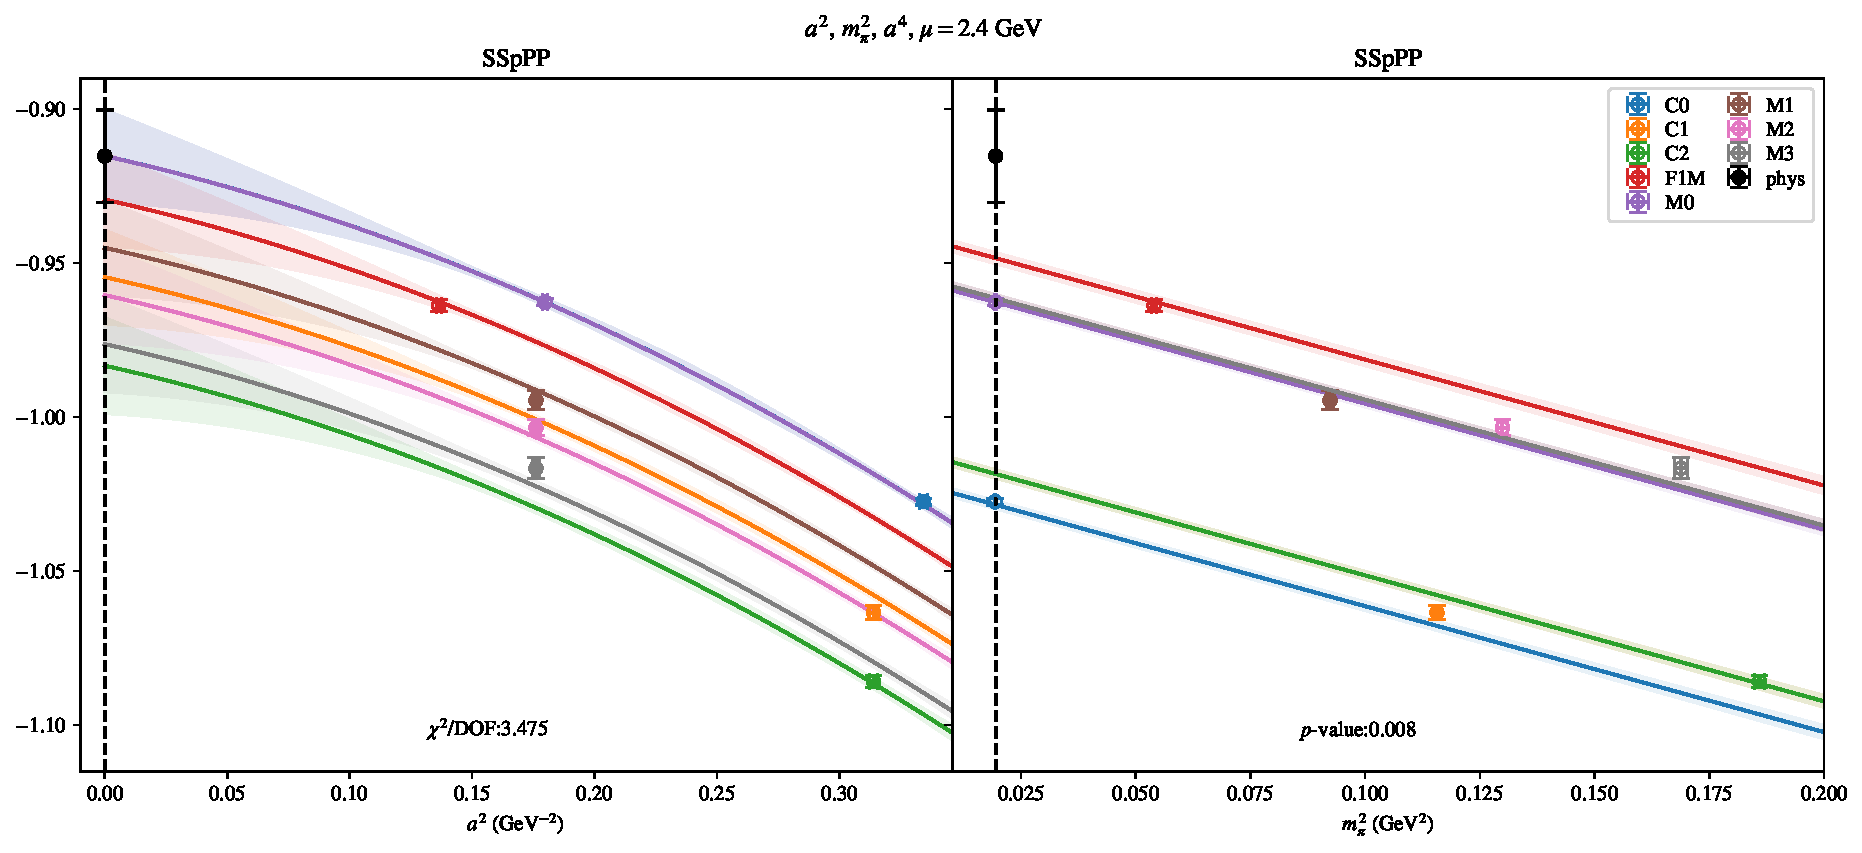
\includepdf[link, pages=-]{VVmAA/SUSY/bag_a2a4m2_24.pdf}
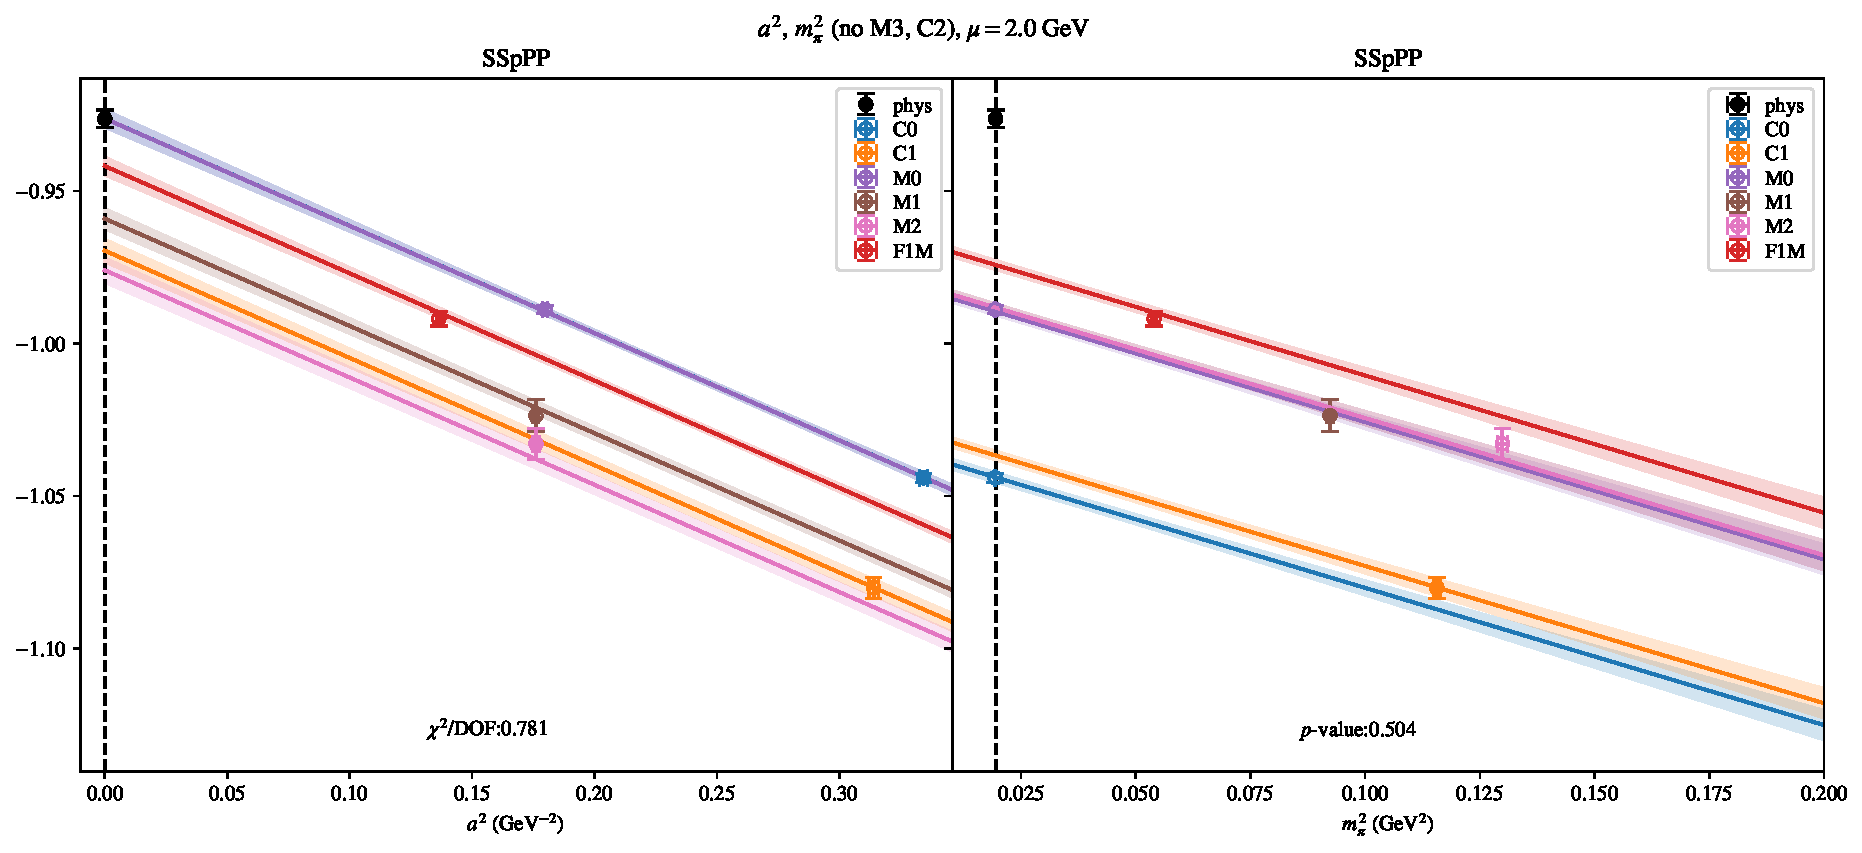
\includepdf[link, pages=-]{VVmAA/SUSY/bag_a2m2mcut_20.pdf}
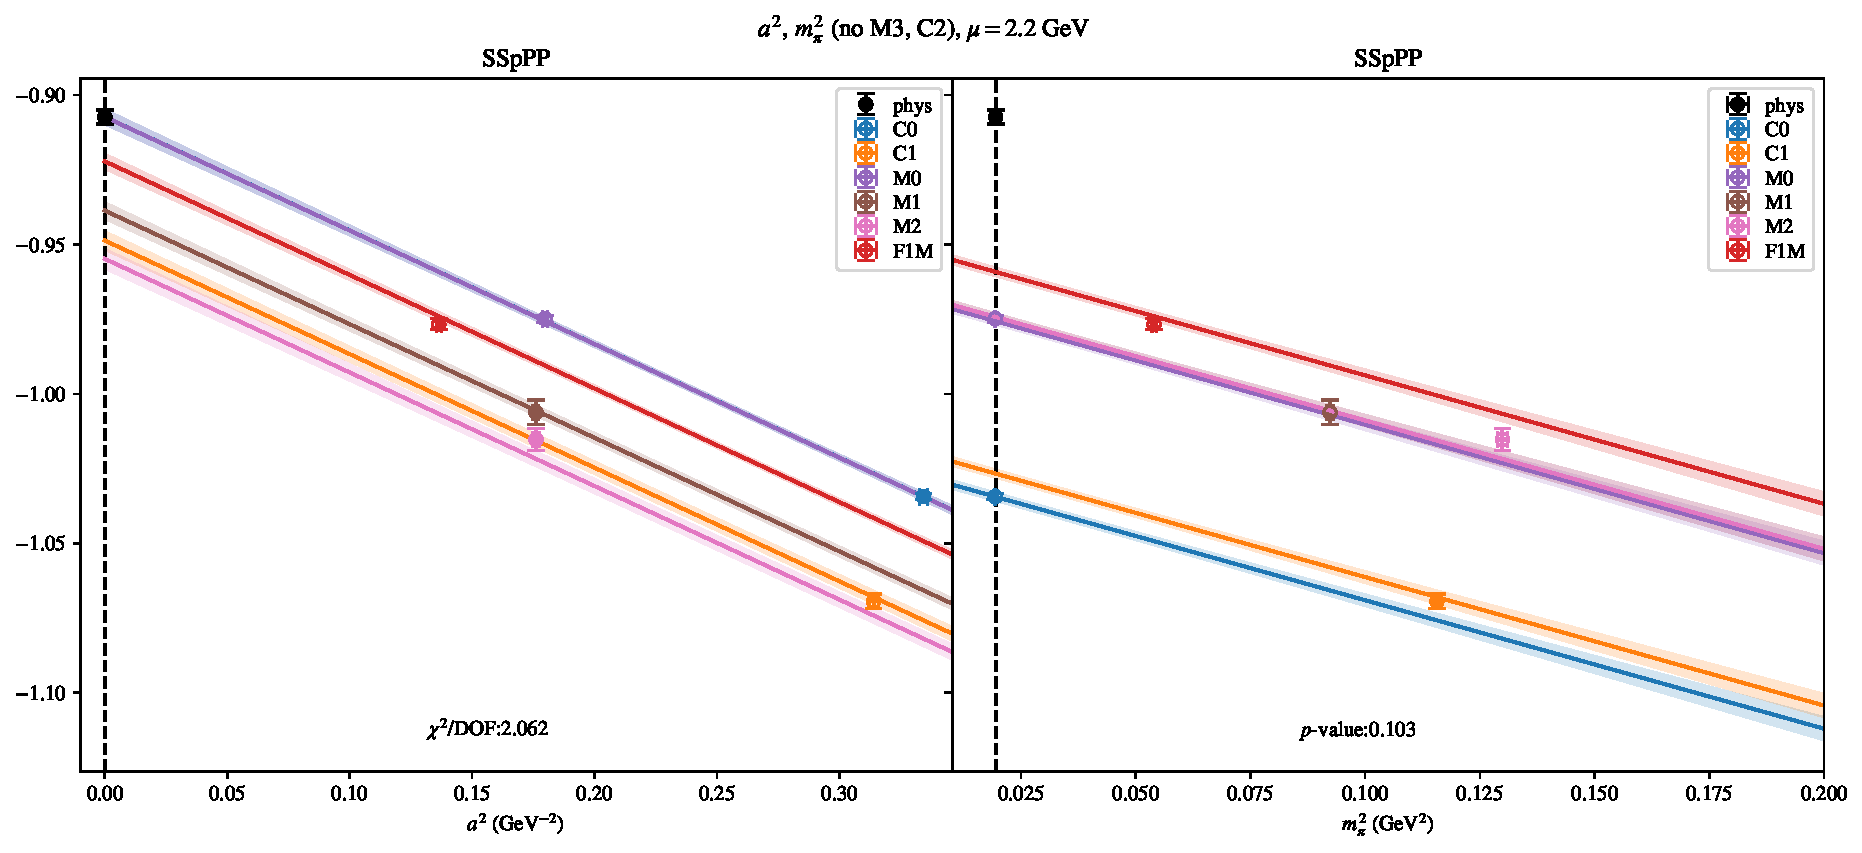
\includepdf[link, pages=-]{VVmAA/SUSY/bag_a2m2mcut_22.pdf}
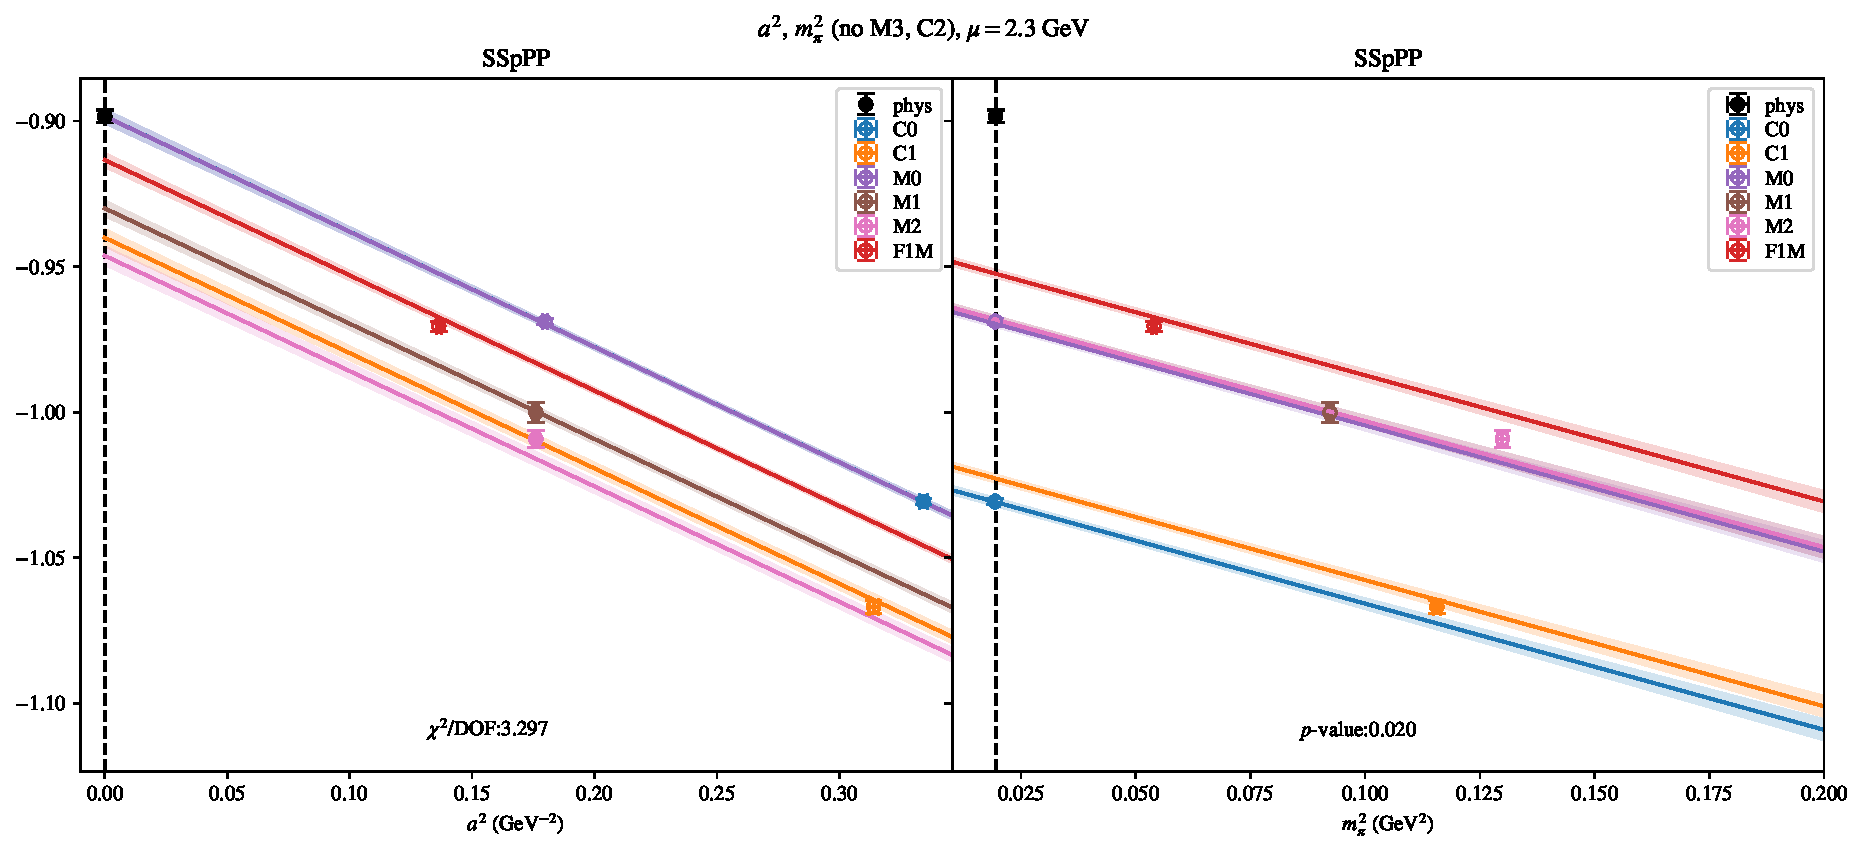
\includepdf[link, pages=-]{VVmAA/SUSY/bag_a2m2mcut_23.pdf}
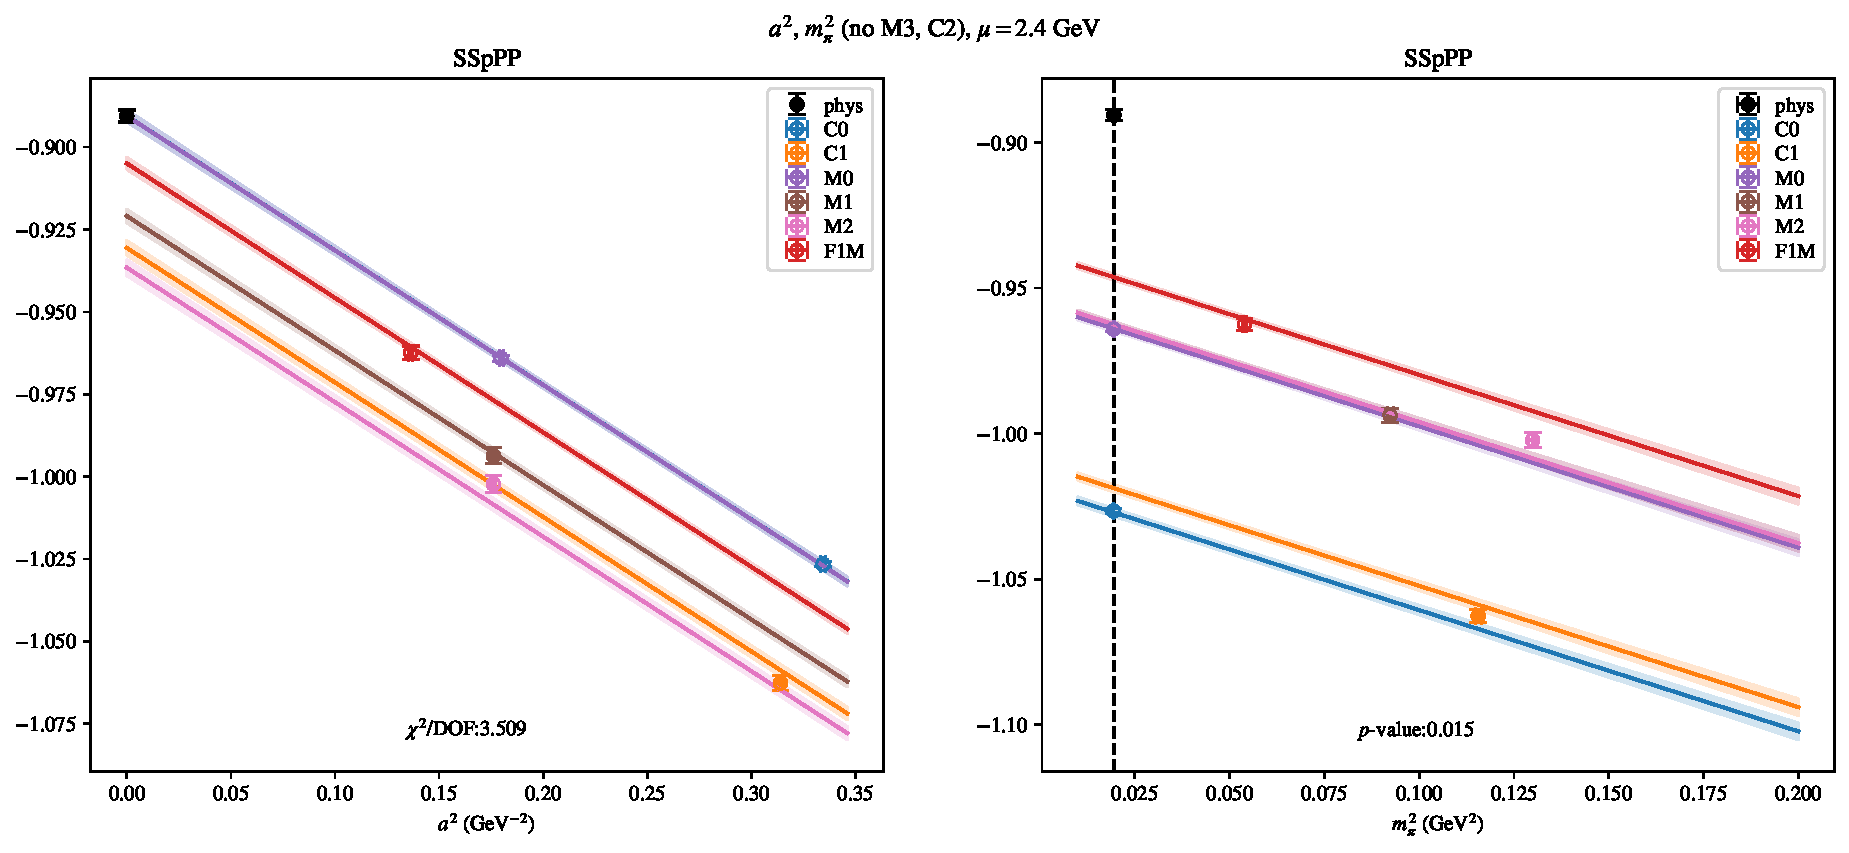
\includepdf[link, pages=-]{VVmAA/SUSY/bag_a2m2mcut_24.pdf}
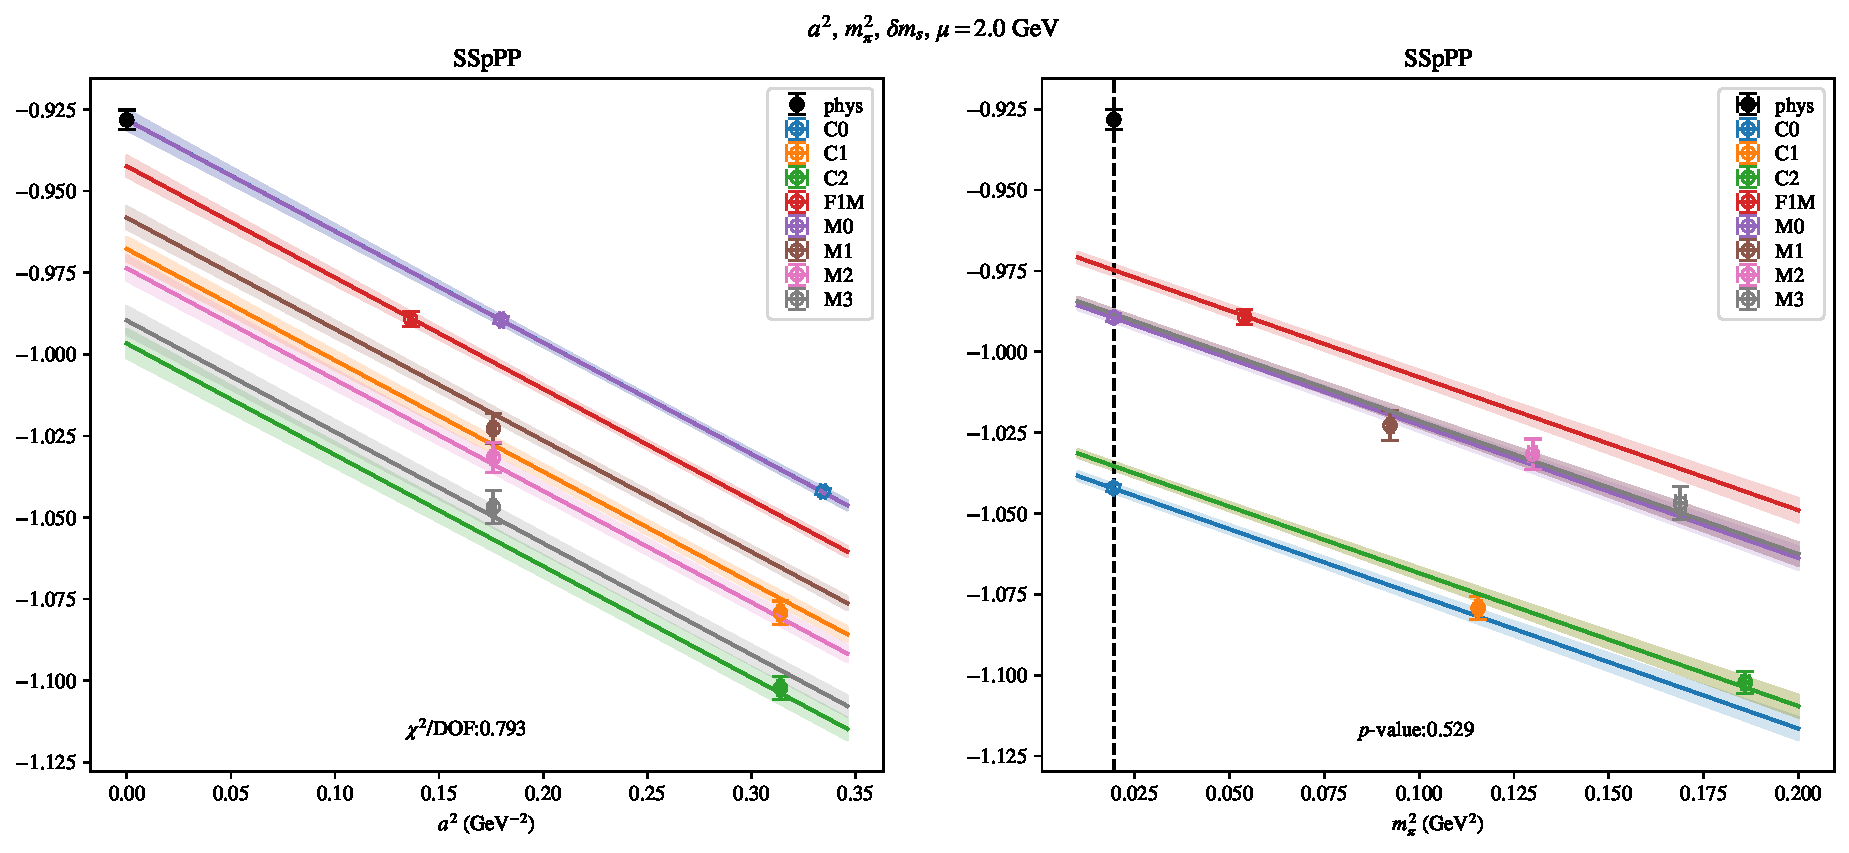
\includepdf[link, pages=-]{VVmAA/SUSY/bag_a2m2delm_20.pdf}
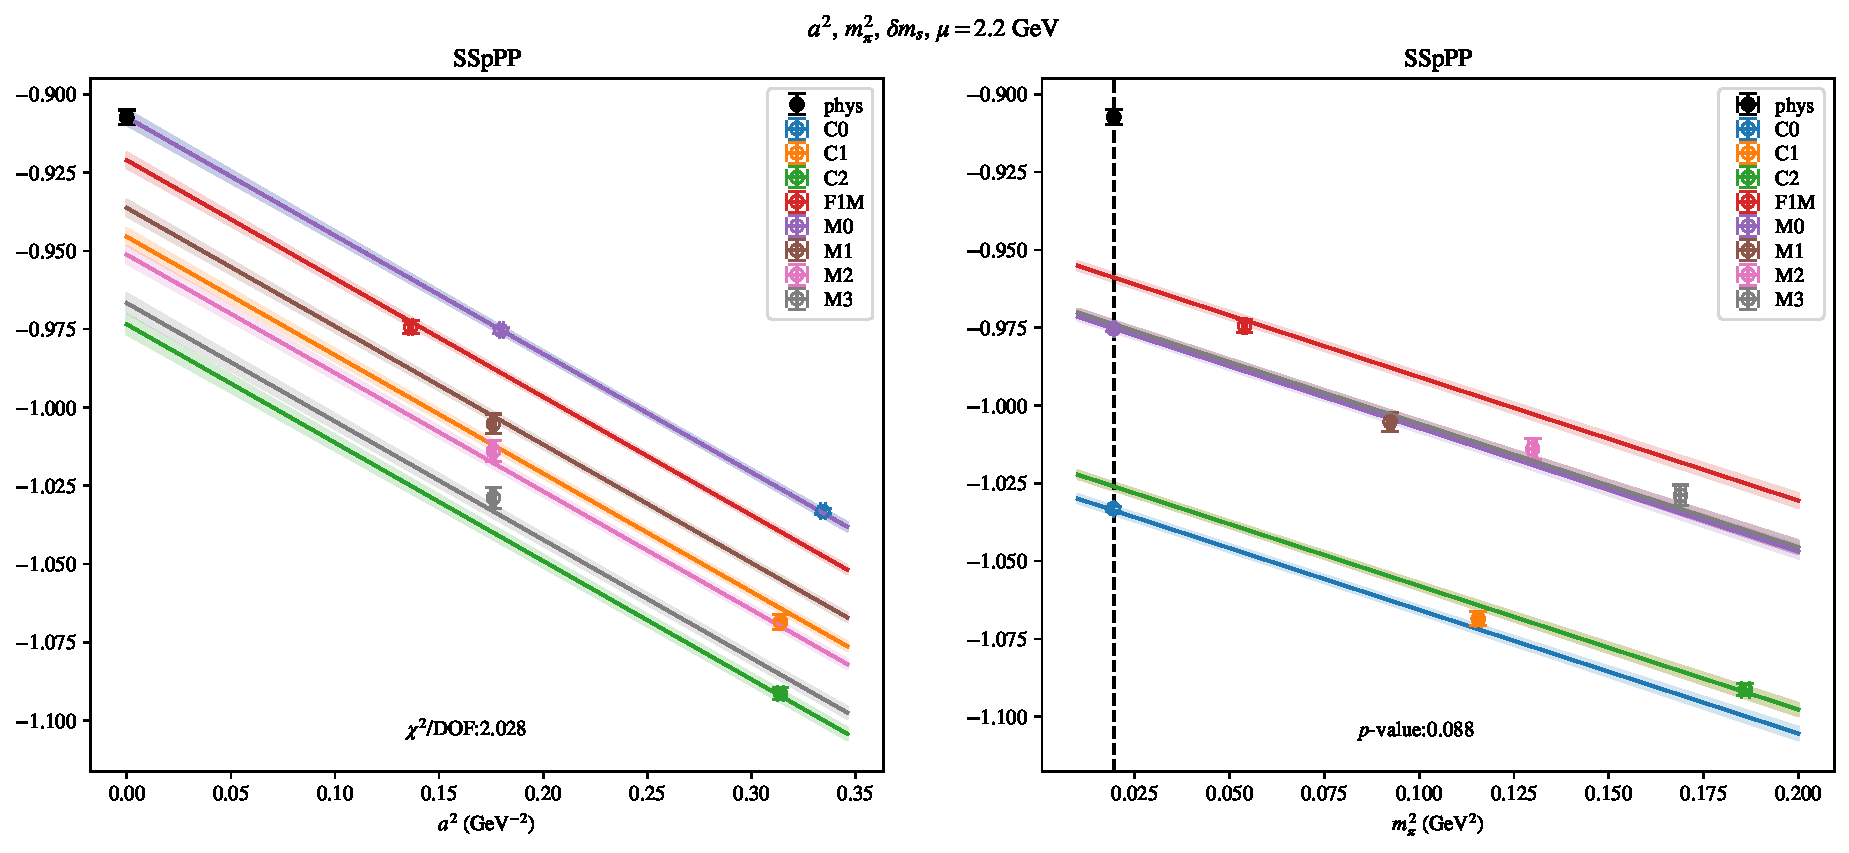
\includepdf[link, pages=-]{VVmAA/SUSY/bag_a2m2delm_22.pdf}
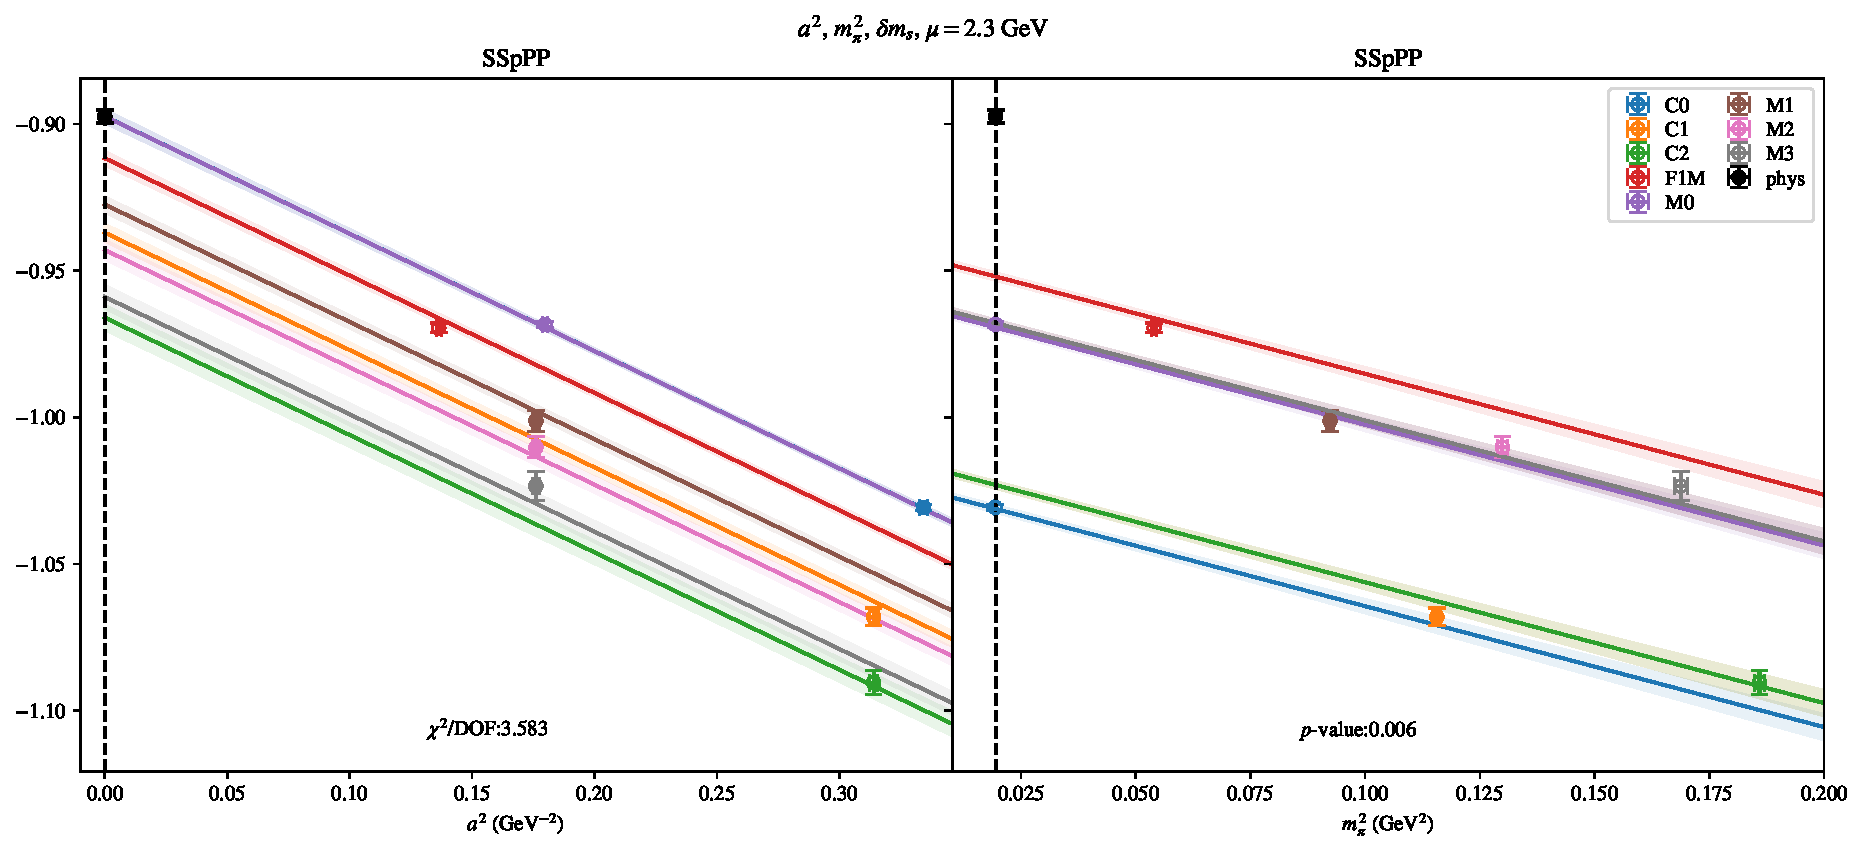
\includepdf[link, pages=-]{VVmAA/SUSY/bag_a2m2delm_23.pdf}
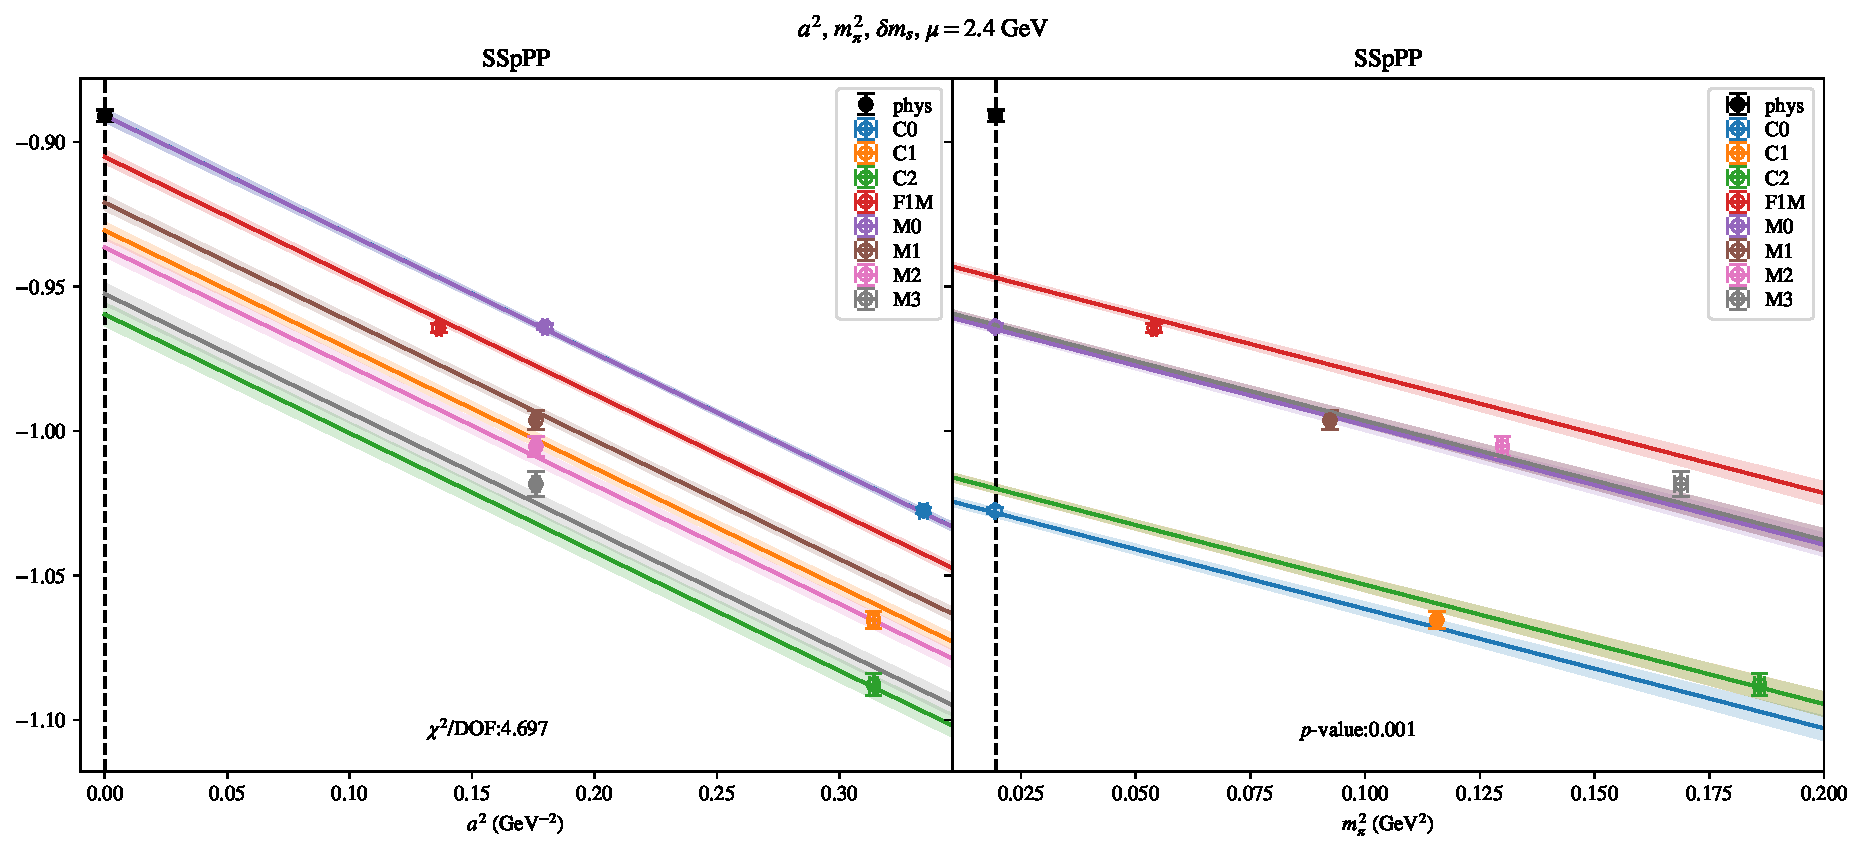
\includepdf[link, pages=-]{VVmAA/SUSY/bag_a2m2delm_24.pdf}
\clearpage
\section{$\mathcal{B}_3$}
\begin{table}[h!]
\begin{center}
\begin{tabular}{|c|c|c|c|c|c|}
\hline
$\mu$ (GeV) & $a^2$, $m_\pi^2$& $a^2$, $m_\pi^2$ (no C)& $a^2$, $m_\pi^2$, $a^4$& $a^2$, $m_\pi^2$ (no M3, C2)& $a^2$, $m_\pi^2$, $\delta m_s$\\
\hline
2.0& \hyperlink{SSmPP/SUSY/bag_a2m2_20.pdf.1}{\textbf{0.2814(60)}: 0.034 (0.999)} & \hyperlink{SSmPP/SUSY/bag_a2m2noC_20.pdf.1}{\textbf{0.284(22)}: 0.042 (0.958)} & \hyperlink{SSmPP/SUSY/bag_a2a4m2_20.pdf.1}{\textbf{0.285(38)}: 0.04 (0.997)} & \hyperlink{SSmPP/SUSY/bag_a2m2mcut_20.pdf.1}{\textbf{0.2807(64)}: 0.017 (0.997)} & \hyperlink{SSmPP/SUSY/bag_a2m2delm_20.pdf.1}{\textbf{0.2815(60)}: 0.042 (0.997)}\\
2.2& \hyperlink{SSmPP/SUSY/bag_a2m2_22.pdf.1}{\textbf{0.2735(52)}: 0.049 (0.999)} & \hyperlink{SSmPP/SUSY/bag_a2m2noC_22.pdf.1}{\textbf{0.278(21)}: 0.043 (0.958)} & \hyperlink{SSmPP/SUSY/bag_a2a4m2_22.pdf.1}{\textbf{0.279(36)}: 0.056 (0.994)} & \hyperlink{SSmPP/SUSY/bag_a2m2mcut_22.pdf.1}{\textbf{0.2730(56)}: 0.032 (0.992)} & \hyperlink{SSmPP/SUSY/bag_a2m2delm_22.pdf.1}{\textbf{0.2735(52)}: 0.06 (0.993)}\\
2.3& \hyperlink{SSmPP/SUSY/bag_a2m2_23.pdf.1}{\textbf{0.2697(47)}: 0.065 (0.997)} & \hyperlink{SSmPP/SUSY/bag_a2m2noC_23.pdf.1}{\textbf{0.275(18)}: 0.047 (0.954)} & \hyperlink{SSmPP/SUSY/bag_a2a4m2_23.pdf.1}{\textbf{0.277(32)}: 0.069 (0.991)} & \hyperlink{SSmPP/SUSY/bag_a2m2mcut_23.pdf.1}{\textbf{0.2692(51)}: 0.05 (0.985)} & \hyperlink{SSmPP/SUSY/bag_a2m2delm_23.pdf.1}{\textbf{0.2697(47)}: 0.082 (0.988)}\\
2.4& \hyperlink{SSmPP/SUSY/bag_a2m2_24.pdf.1}{\textbf{0.2662(45)}: 0.086 (0.994)} & \hyperlink{SSmPP/SUSY/bag_a2m2noC_24.pdf.1}{\textbf{0.273(17)}: 0.058 (0.944)} & \hyperlink{SSmPP/SUSY/bag_a2a4m2_24.pdf.1}{\textbf{0.274(29)}: 0.091 (0.985)} & \hyperlink{SSmPP/SUSY/bag_a2m2mcut_24.pdf.1}{\textbf{0.2659(48)}: 0.07 (0.976)} & \hyperlink{SSmPP/SUSY/bag_a2m2delm_24.pdf.1}{\textbf{0.2662(45)}: 0.108 (0.98)}\\
\hline
\end{tabular}
\caption{Physical point value from chiral and continuum extrapolation at renormalisation scale $\mu$. Entries are \textbf{value(error)}: $\chi^2/\text{DOF}$ ($p$-value).}
\end{center}
\end{table}
\begin{table}[h!]
\begin{center}
\begin{tabular}{|c c|c|c|c|c|c|}
\hline
$\mu$ (GeV) &  & $a^2$, $m_\pi^2$& $a^2$, $m_\pi^2$ (no C)& $a^2$, $m_\pi^2$, $a^4$& $a^2$, $m_\pi^2$ (no M3, C2)& $a^2$, $m_\pi^2$, $\delta m_s$\\
\hline
\multirow{3}{0.5in}{2.0} & $\alpha$ & 0.182(21)& 0.17(13)& 0.14(35)& 0.184(22)& 0.182(21)\\
 & $\beta$ & 0.00232(62)& 0.0024(10)& 0.00233(63)& 0.0026(10)& 0.0022(10)\\
 & $\gamma$ &  &  & 0.08(72)&  & 0.003(36)\\
\hline
\multirow{3}{0.5in}{2.2} & $\alpha$ & 0.204(18)& 0.18(12)& 0.15(33)& 0.206(19)& 0.204(18)\\
 & $\beta$ & 0.00224(49)& 0.00218(87)& 0.00226(52)& 0.00249(84)& 0.00217(95)\\
 & $\gamma$ &  &  & 0.10(67)&  & 0.003(31)\\
\hline
\multirow{3}{0.5in}{2.3} & $\alpha$ & 0.216(16)& 0.18(10)& 0.15(29)& 0.217(17)& 0.216(16)\\
 & $\beta$ & 0.00225(46)& 0.00216(77)& 0.00228(48)& 0.00249(77)& 0.00225(86)\\
 & $\gamma$ &  &  & 0.13(60)&  & -0.0002(283)\\
\hline
\multirow{3}{0.5in}{2.4} & $\alpha$ & 0.227(16)& 0.19(10)& 0.16(27)& 0.228(16)& 0.227(16)\\
 & $\beta$ & 0.00224(41)& 0.00212(69)& 0.00227(43)& 0.00247(71)& 0.00224(80)\\
 & $\gamma$ &  &  & 0.14(55)&  & -0.0002(268)\\
\hline
\end{tabular}
\caption{Fit values of coefficients in $Q = Q_{phys} + \mathbf{\alpha} a^2 + \mathbf{\beta}\left(\frac{m_\pi^2}{f_\pi^2}-\frac{m_{\pi,PDG}^2}{f_\pi^2}\right) + \gamma(\ldots)$}
\end{center}
\end{table}
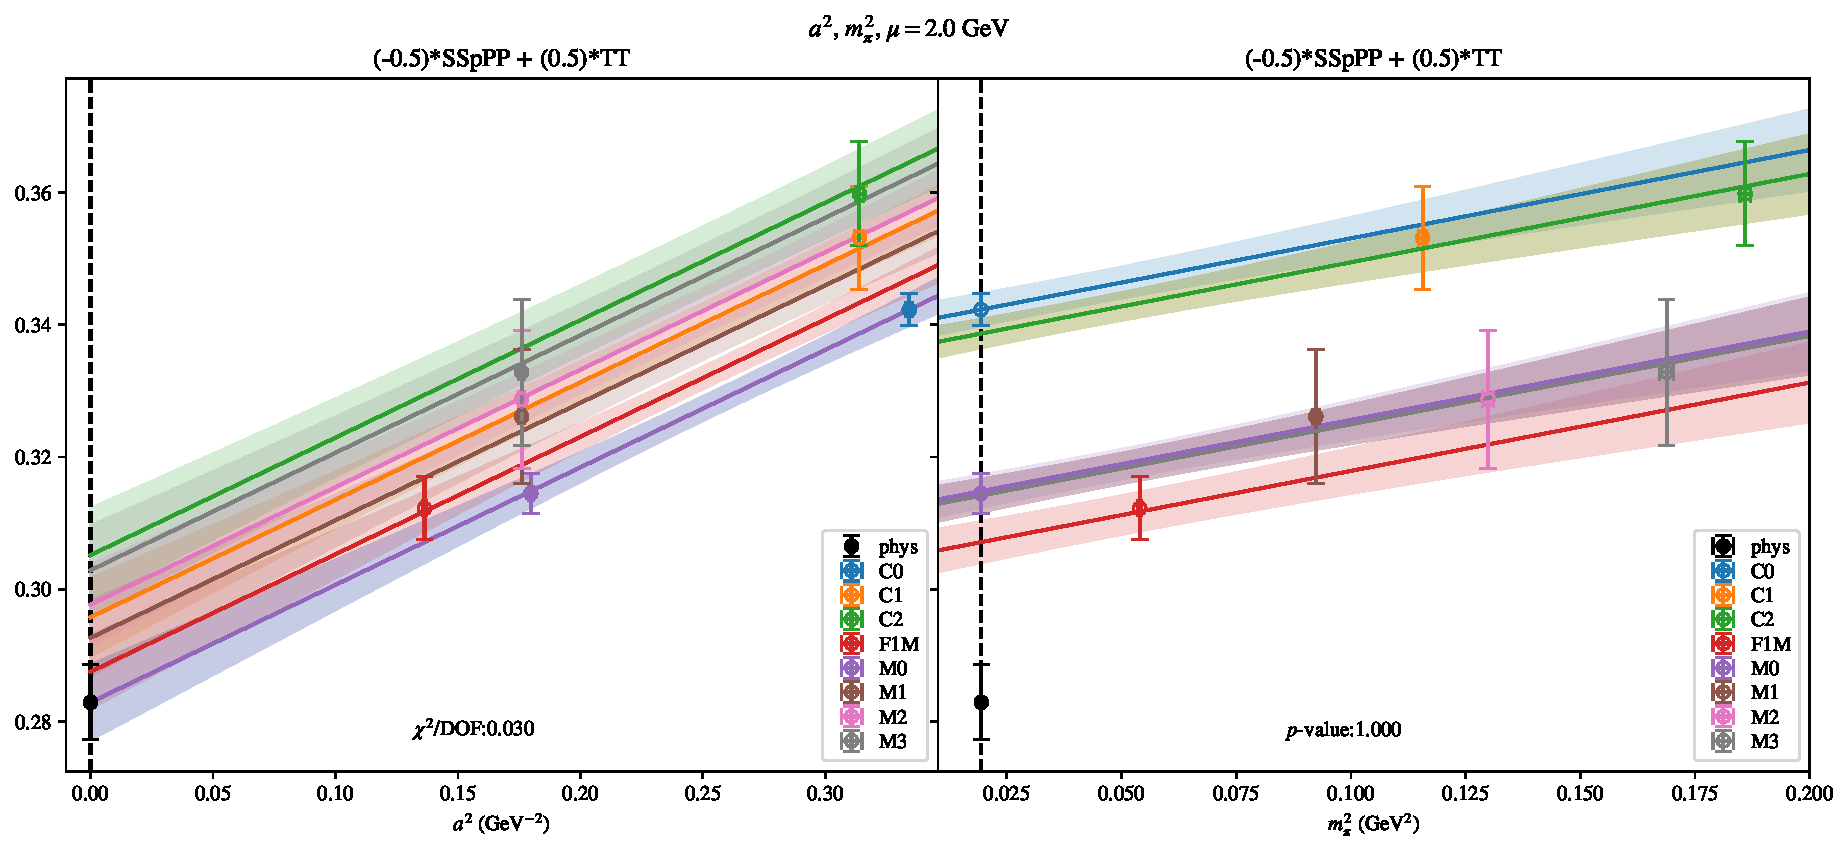
\includepdf[link, pages=-]{SSmPP/SUSY/bag_a2m2_20.pdf}
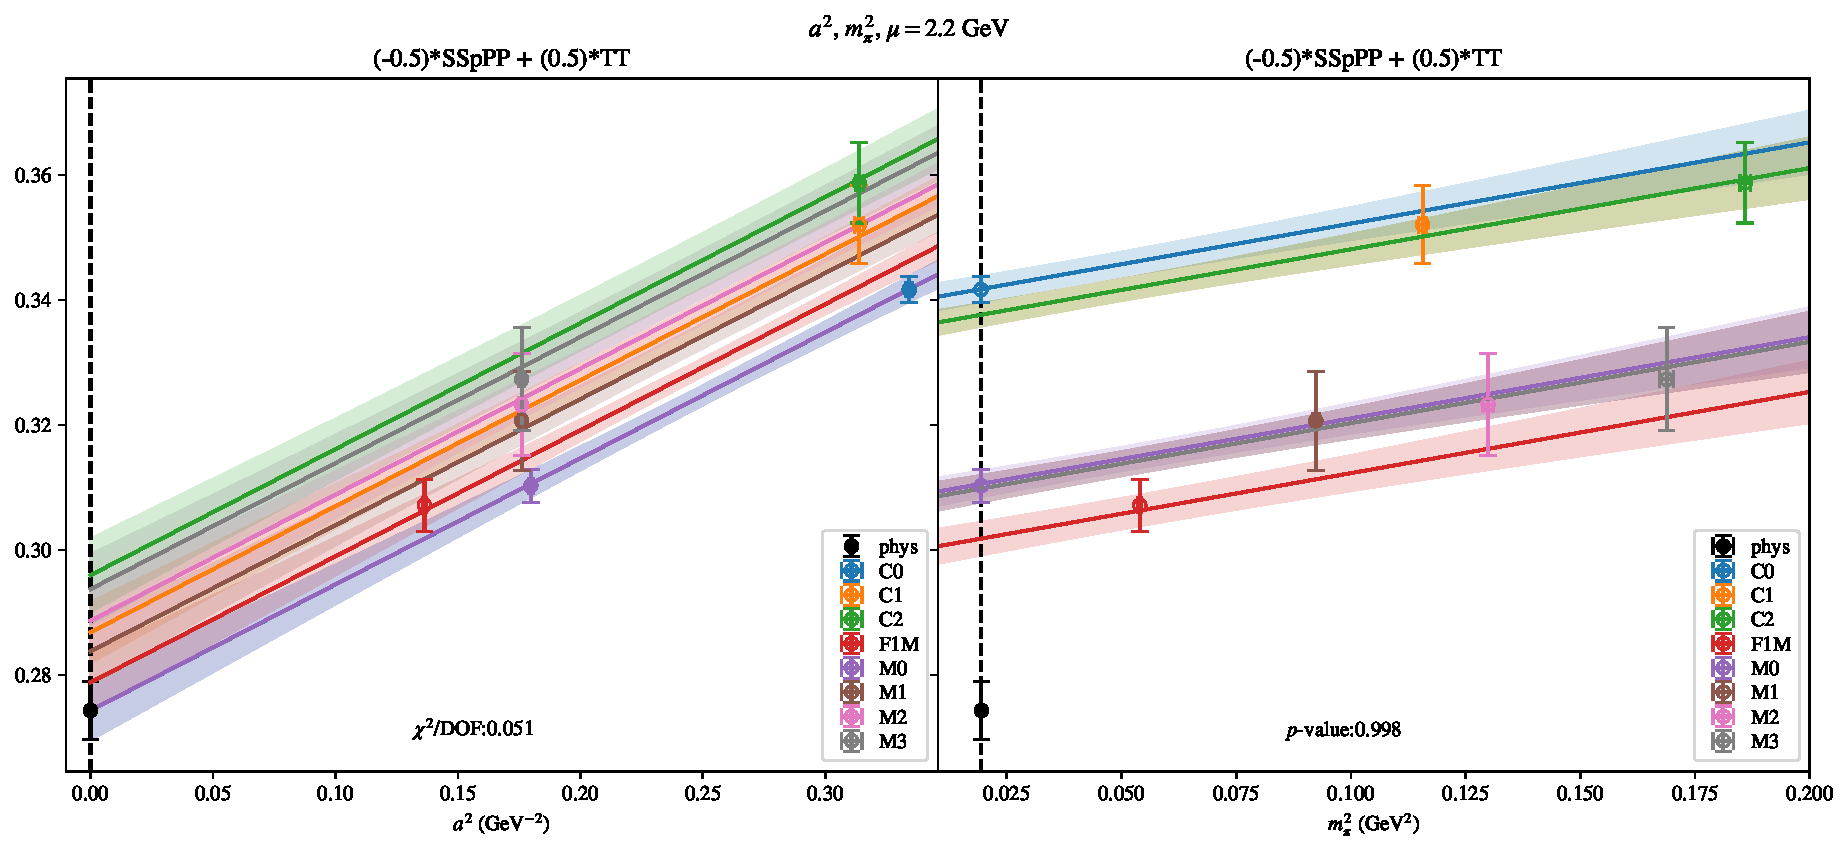
\includepdf[link, pages=-]{SSmPP/SUSY/bag_a2m2_22.pdf}
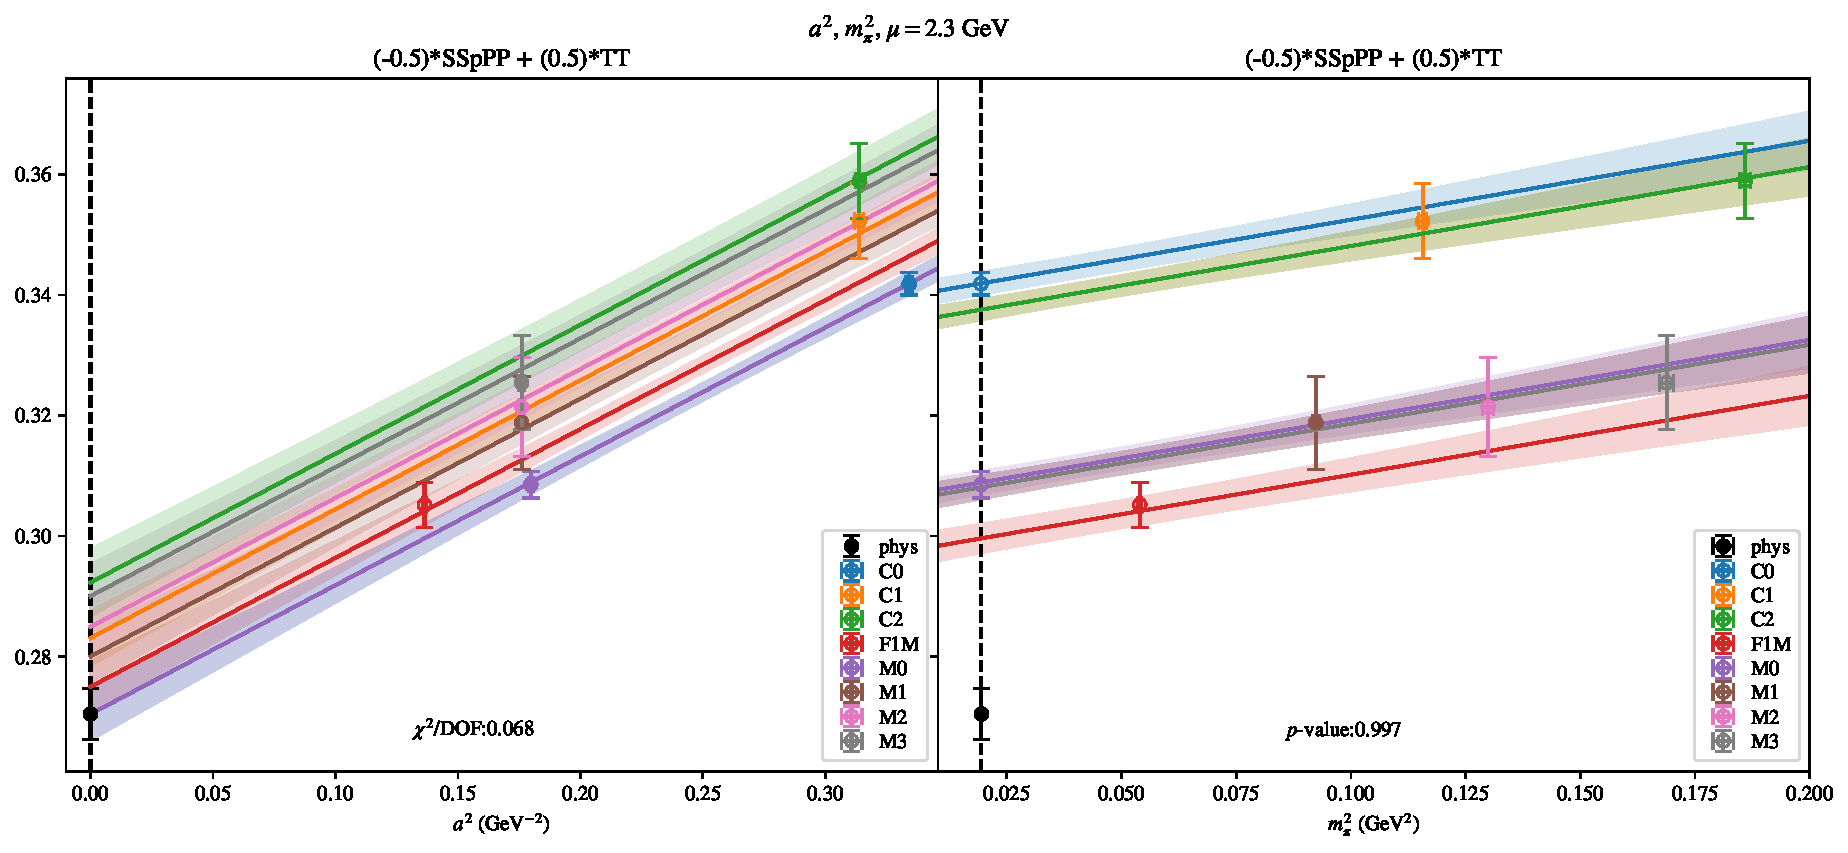
\includepdf[link, pages=-]{SSmPP/SUSY/bag_a2m2_23.pdf}
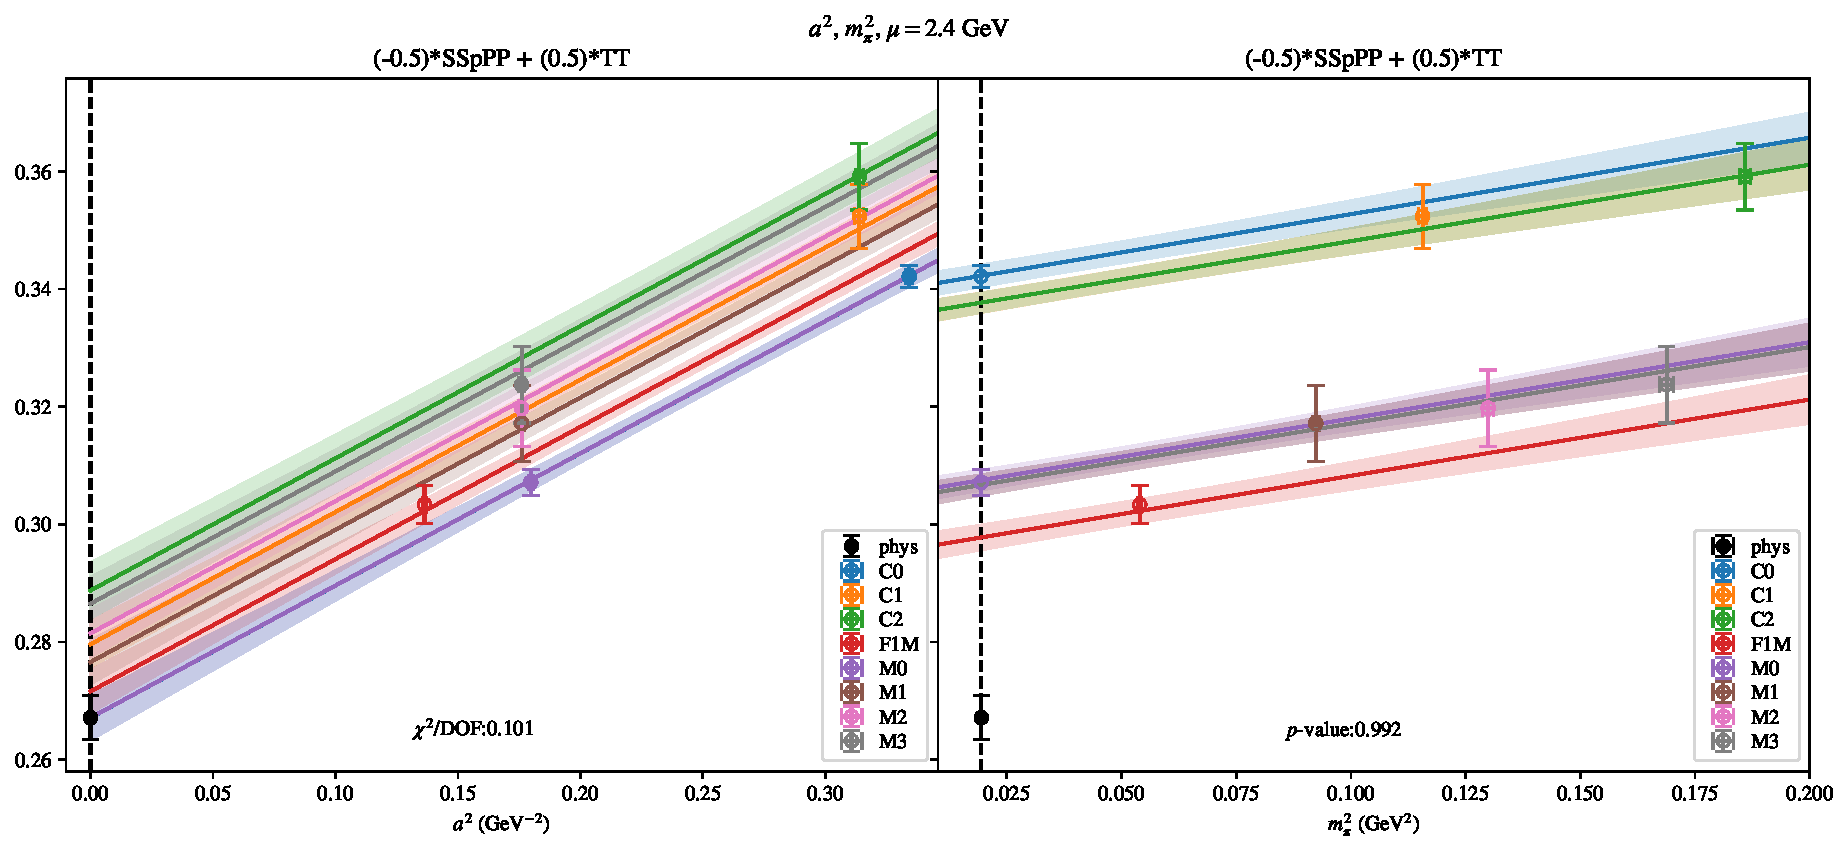
\includepdf[link, pages=-]{SSmPP/SUSY/bag_a2m2_24.pdf}
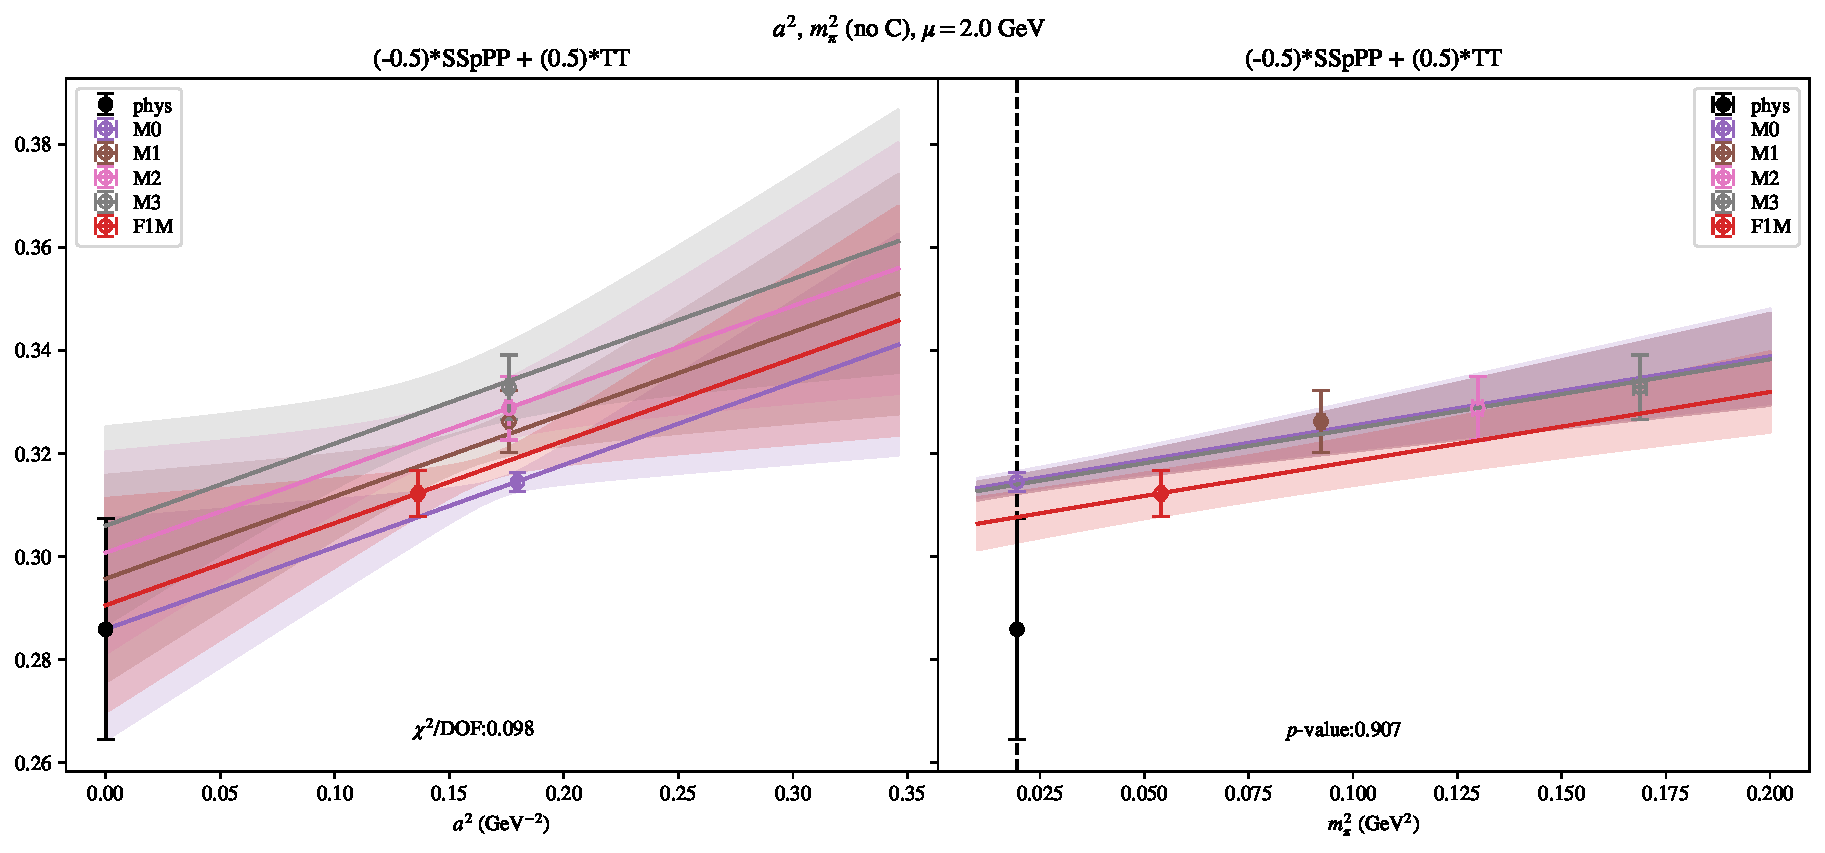
\includepdf[link, pages=-]{SSmPP/SUSY/bag_a2m2noC_20.pdf}
\includepdf[link, pages=-]{SSmPP/SUSY/bag_a2m2noC_22.pdf}
\includepdf[link, pages=-]{SSmPP/SUSY/bag_a2m2noC_23.pdf}
\includepdf[link, pages=-]{SSmPP/SUSY/bag_a2m2noC_24.pdf}
\includepdf[link, pages=-]{SSmPP/SUSY/bag_a2a4m2_20.pdf}
\includepdf[link, pages=-]{SSmPP/SUSY/bag_a2a4m2_22.pdf}
\includepdf[link, pages=-]{SSmPP/SUSY/bag_a2a4m2_23.pdf}
\includepdf[link, pages=-]{SSmPP/SUSY/bag_a2a4m2_24.pdf}
\includepdf[link, pages=-]{SSmPP/SUSY/bag_a2m2mcut_20.pdf}
\includepdf[link, pages=-]{SSmPP/SUSY/bag_a2m2mcut_22.pdf}
\includepdf[link, pages=-]{SSmPP/SUSY/bag_a2m2mcut_23.pdf}
\includepdf[link, pages=-]{SSmPP/SUSY/bag_a2m2mcut_24.pdf}
\includepdf[link, pages=-]{SSmPP/SUSY/bag_a2m2delm_20.pdf}
\includepdf[link, pages=-]{SSmPP/SUSY/bag_a2m2delm_22.pdf}
\includepdf[link, pages=-]{SSmPP/SUSY/bag_a2m2delm_23.pdf}
\includepdf[link, pages=-]{SSmPP/SUSY/bag_a2m2delm_24.pdf}
\clearpage
\section{$\mathcal{B}_4$}
\begin{table}[h!]
\begin{center}
\begin{tabular}{|c|c|c|c|c|c|}
\hline
$\mu$ (GeV) & $a^2$, $m_\pi^2$& $a^2$, $m_\pi^2$ (no C)& $a^2$, $m_\pi^2$, $a^4$& $a^2$, $m_\pi^2$ (no M3, C2)& $a^2$, $m_\pi^2$, $\delta m_s$\\
\hline
2.0& \hyperlink{SSpPP/SUSY/bag_a2m2_20.pdf.1}{\textbf{1.7967(44)}: 4.285 (0.001)} & \hyperlink{SSpPP/SUSY/bag_a2m2noC_20.pdf.1}{\textbf{1.695(22)}: 0.067 (0.935)} & \hyperlink{SSpPP/SUSY/bag_a2a4m2_20.pdf.1}{\textbf{1.654(35)}: 1.23 (0.296)} & \hyperlink{SSpPP/SUSY/bag_a2m2mcut_20.pdf.1}{\textbf{1.7965(46)}: 6.74 (0.0)} & \hyperlink{SSpPP/SUSY/bag_a2m2delm_20.pdf.1}{\textbf{1.7928(52)}: 2.348 (0.052)}\\
2.2& \hyperlink{SSpPP/SUSY/bag_a2m2_22.pdf.1}{\textbf{1.8005(37)}: 6.632 (0.0)} & \hyperlink{SSpPP/SUSY/bag_a2m2noC_22.pdf.1}{\textbf{1.714(15)}: 0.128 (0.88)} & \hyperlink{SSpPP/SUSY/bag_a2a4m2_22.pdf.1}{\textbf{1.665(26)}: 1.13 (0.34)} & \hyperlink{SSpPP/SUSY/bag_a2m2mcut_22.pdf.1}{\textbf{1.8012(40)}: 10.429 (0.0)} & \hyperlink{SSpPP/SUSY/bag_a2m2delm_22.pdf.1}{\textbf{1.8000(43)}: 3.99 (0.003)}\\
2.3& \hyperlink{SSpPP/SUSY/bag_a2m2_23.pdf.1}{\textbf{1.8015(35)}: 7.153 (0.0)} & \hyperlink{SSpPP/SUSY/bag_a2m2noC_23.pdf.1}{\textbf{1.719(14)}: 0.161 (0.851)} & \hyperlink{SSpPP/SUSY/bag_a2a4m2_23.pdf.1}{\textbf{1.666(24)}: 0.821 (0.511)} & \hyperlink{SSpPP/SUSY/bag_a2m2mcut_23.pdf.1}{\textbf{1.8022(37)}: 11.483 (0.0)} & \hyperlink{SSpPP/SUSY/bag_a2m2delm_23.pdf.1}{\textbf{1.8014(41)}: 4.025 (0.003)}\\
2.4& \hyperlink{SSpPP/SUSY/bag_a2m2_24.pdf.1}{\textbf{1.8037(34)}: 6.49 (0.0)} & \hyperlink{SSpPP/SUSY/bag_a2m2noC_24.pdf.1}{\textbf{1.722(14)}: 0.19 (0.827)} & \hyperlink{SSpPP/SUSY/bag_a2a4m2_24.pdf.1}{\textbf{1.674(25)}: 0.989 (0.412)} & \hyperlink{SSpPP/SUSY/bag_a2m2mcut_24.pdf.1}{\textbf{1.8040(38)}: 10.577 (0.0)} & \hyperlink{SSpPP/SUSY/bag_a2m2delm_24.pdf.1}{\textbf{1.8030(39)}: 4.158 (0.002)}\\
\hline
\end{tabular}
\caption{Physical point value from chiral and continuum extrapolation at renormalisation scale $\mu$. Entries are \textbf{value(error)}: $\chi^2/\text{DOF}$ ($p$-value).}
\end{center}
\end{table}
\begin{table}[h!]
\begin{center}
\begin{tabular}{|c c|c|c|c|c|c|}
\hline
$\mu$ (GeV) &  & $a^2$, $m_\pi^2$& $a^2$, $m_\pi^2$ (no C)& $a^2$, $m_\pi^2$, $a^4$& $a^2$, $m_\pi^2$ (no M3, C2)& $a^2$, $m_\pi^2$, $\delta m_s$\\
\hline
\multirow{3}{0.5in}{2.0} & $\alpha$ & 0.145(17)& 0.72(12)& 1.41(31)& 0.146(18)& 0.147(19)\\
 & $\beta$ & -0.00043(43)& 0.00057(80)& -0.00075(44)& -0.00089(76)& -0.00318(91)\\
 & $\gamma$ &  &  & -2.53(62)&  & 0.113(32)\\
\hline
\multirow{3}{0.5in}{2.2} & $\alpha$ & 0.152(13)& 0.664(91)& 1.39(23)& 0.150(14)& 0.147(15)\\
 & $\beta$ & -0.00067(31)& -0.00039(63)& -0.00123(33)& -0.00121(54)& -0.00315(69)\\
 & $\gamma$ &  &  & -2.51(47)&  & 0.097(23)\\
\hline
\multirow{3}{0.5in}{2.3} & $\alpha$ & 0.157(12)& 0.652(84)& 1.40(22)& 0.156(13)& 0.151(15)\\
 & $\beta$ & -0.00039(29)& -0.00035(57)& -0.00095(31)& -0.00082(51)& -0.00284(67)\\
 & $\gamma$ &  &  & -2.53(44)&  & 0.097(23)\\
\hline
\multirow{3}{0.5in}{2.4} & $\alpha$ & 0.158(12)& 0.640(85)& 1.35(22)& 0.157(14)& 0.153(14)\\
 & $\beta$ & -0.00027(26)& -0.00020(52)& -0.00082(29)& -0.00052(45)& -0.00238(62)\\
 & $\gamma$ &  &  & -2.41(45)&  & 0.084(21)\\
\hline
\end{tabular}
\caption{Fit values of coefficients in $Q = Q_{phys} + \mathbf{\alpha} a^2 + \mathbf{\beta}\left(\frac{m_\pi^2}{f_\pi^2}-\frac{m_{\pi,PDG}^2}{f_\pi^2}\right) + \gamma(\ldots)$}
\end{center}
\end{table}
\includepdf[link, pages=-]{SSpPP/SUSY/bag_a2m2_20.pdf}
\includepdf[link, pages=-]{SSpPP/SUSY/bag_a2m2_22.pdf}
\includepdf[link, pages=-]{SSpPP/SUSY/bag_a2m2_23.pdf}
\includepdf[link, pages=-]{SSpPP/SUSY/bag_a2m2_24.pdf}
\includepdf[link, pages=-]{SSpPP/SUSY/bag_a2m2noC_20.pdf}
\includepdf[link, pages=-]{SSpPP/SUSY/bag_a2m2noC_22.pdf}
\includepdf[link, pages=-]{SSpPP/SUSY/bag_a2m2noC_23.pdf}
\includepdf[link, pages=-]{SSpPP/SUSY/bag_a2m2noC_24.pdf}
\includepdf[link, pages=-]{SSpPP/SUSY/bag_a2a4m2_20.pdf}
\includepdf[link, pages=-]{SSpPP/SUSY/bag_a2a4m2_22.pdf}
\includepdf[link, pages=-]{SSpPP/SUSY/bag_a2a4m2_23.pdf}
\includepdf[link, pages=-]{SSpPP/SUSY/bag_a2a4m2_24.pdf}
\includepdf[link, pages=-]{SSpPP/SUSY/bag_a2m2mcut_20.pdf}
\includepdf[link, pages=-]{SSpPP/SUSY/bag_a2m2mcut_22.pdf}
\includepdf[link, pages=-]{SSpPP/SUSY/bag_a2m2mcut_23.pdf}
\includepdf[link, pages=-]{SSpPP/SUSY/bag_a2m2mcut_24.pdf}
\includepdf[link, pages=-]{SSpPP/SUSY/bag_a2m2delm_20.pdf}
\includepdf[link, pages=-]{SSpPP/SUSY/bag_a2m2delm_22.pdf}
\includepdf[link, pages=-]{SSpPP/SUSY/bag_a2m2delm_23.pdf}
\includepdf[link, pages=-]{SSpPP/SUSY/bag_a2m2delm_24.pdf}
\clearpage
\section{$\mathcal{B}_5$}
\begin{table}[h!]
\begin{center}
\begin{tabular}{|c|c|c|c|c|c|}
\hline
$\mu$ (GeV) & $a^2$, $m_\pi^2$& $a^2$, $m_\pi^2$ (no C)& $a^2$, $m_\pi^2$, $a^4$& $a^2$, $m_\pi^2$ (no M3, C2)& $a^2$, $m_\pi^2$, $\delta m_s$\\
\hline
2.0& \hyperlink{TT/SUSY/bag_a2m2_20.pdf.1}{\textbf{0.4919(67)}: 0.16 (0.977)} & \hyperlink{TT/SUSY/bag_a2m2noC_20.pdf.1}{\textbf{0.470(26)}: 0.003 (0.997)} & \hyperlink{TT/SUSY/bag_a2a4m2_20.pdf.1}{\textbf{0.458(43)}: 0.045 (0.996)} & \hyperlink{TT/SUSY/bag_a2m2mcut_20.pdf.1}{\textbf{0.4919(71)}: 0.244 (0.866)} & \hyperlink{TT/SUSY/bag_a2m2delm_20.pdf.1}{\textbf{0.4923(67)}: 0.093 (0.985)}\\
2.2& \hyperlink{TT/SUSY/bag_a2m2_22.pdf.1}{\textbf{0.5000(56)}: 0.157 (0.978)} & \hyperlink{TT/SUSY/bag_a2m2noC_22.pdf.1}{\textbf{0.481(23)}: 0.008 (0.992)} & \hyperlink{TT/SUSY/bag_a2a4m2_22.pdf.1}{\textbf{0.469(39)}: 0.033 (0.998)} & \hyperlink{TT/SUSY/bag_a2m2mcut_22.pdf.1}{\textbf{0.5003(61)}: 0.238 (0.87)} & \hyperlink{TT/SUSY/bag_a2m2delm_22.pdf.1}{\textbf{0.5002(56)}: 0.111 (0.979)}\\
2.3& \hyperlink{TT/SUSY/bag_a2m2_23.pdf.1}{\textbf{0.5027(52)}: 0.176 (0.971)} & \hyperlink{TT/SUSY/bag_a2m2noC_23.pdf.1}{\textbf{0.484(21)}: 0.008 (0.992)} & \hyperlink{TT/SUSY/bag_a2a4m2_23.pdf.1}{\textbf{0.470(37)}: 0.021 (0.999)} & \hyperlink{TT/SUSY/bag_a2m2mcut_23.pdf.1}{\textbf{0.5030(57)}: 0.277 (0.842)} & \hyperlink{TT/SUSY/bag_a2m2delm_23.pdf.1}{\textbf{0.5030(53)}: 0.105 (0.981)}\\
2.4& \hyperlink{TT/SUSY/bag_a2m2_24.pdf.1}{\textbf{0.5049(47)}: 0.191 (0.966)} & \hyperlink{TT/SUSY/bag_a2m2noC_24.pdf.1}{\textbf{0.487(19)}: 0.009 (0.991)} & \hyperlink{TT/SUSY/bag_a2a4m2_24.pdf.1}{\textbf{0.474(34)}: 0.027 (0.999)} & \hyperlink{TT/SUSY/bag_a2m2mcut_24.pdf.1}{\textbf{0.5051(53)}: 0.304 (0.822)} & \hyperlink{TT/SUSY/bag_a2m2delm_24.pdf.1}{\textbf{0.5052(47)}: 0.12 (0.975)}\\
\hline
\end{tabular}
\caption{Physical point value from chiral and continuum extrapolation at renormalisation scale $\mu$. Entries are \textbf{value(error)}: $\chi^2/\text{DOF}$ ($p$-value).}
\end{center}
\end{table}
\begin{table}[h!]
\begin{center}
\begin{tabular}{|c c|c|c|c|c|c|}
\hline
$\mu$ (GeV) &  & $a^2$, $m_\pi^2$& $a^2$, $m_\pi^2$ (no C)& $a^2$, $m_\pi^2$, $a^4$& $a^2$, $m_\pi^2$ (no M3, C2)& $a^2$, $m_\pi^2$, $\delta m_s$\\
\hline
\multirow{3}{0.5in}{2.0} & $\alpha$ & -0.076(23)& 0.06(15)& 0.24(39)& -0.075(24)& -0.079(23)\\
 & $\beta$ & 0.00099(62)& 0.0012(10)& 0.00084(64)& 0.0009(10)& 0.0003(11)\\
 & $\gamma$ &  &  & -0.64(80)&  & 0.027(37)\\
\hline
\multirow{3}{0.5in}{2.2} & $\alpha$ & -0.103(19)& 0.01(13)& 0.19(36)& -0.104(20)& -0.104(19)\\
 & $\beta$ & 0.00082(50)& 0.00082(94)& 0.00067(53)& 0.00064(86)& 0.0003(10)\\
 & $\gamma$ &  &  & -0.59(73)&  & 0.021(33)\\
\hline
\multirow{3}{0.5in}{2.3} & $\alpha$ & -0.114(17)& 0.002(126)& 0.19(33)& -0.115(19)& -0.116(17)\\
 & $\beta$ & 0.00090(49)& 0.00083(87)& 0.00074(53)& 0.00075(83)& 0.00029(99)\\
 & $\gamma$ &  &  & -0.61(68)&  & 0.023(32)\\
\hline
\multirow{3}{0.5in}{2.4} & $\alpha$ & -0.124(16)& -0.01(11)& 0.16(31)& -0.125(17)& -0.126(16)\\
 & $\beta$ & 0.00091(43)& 0.00086(78)& 0.00075(47)& 0.00080(75)& 0.00035(89)\\
 & $\gamma$ &  &  & -0.58(64)&  & 0.021(29)\\
\hline
\end{tabular}
\caption{Fit values of coefficients in $Q = Q_{phys} + \mathbf{\alpha} a^2 + \mathbf{\beta}\left(\frac{m_\pi^2}{f_\pi^2}-\frac{m_{\pi,PDG}^2}{f_\pi^2}\right) + \gamma(\ldots)$}
\end{center}
\end{table}
\includepdf[link, pages=-]{TT/SUSY/bag_a2m2_20.pdf}
\includepdf[link, pages=-]{TT/SUSY/bag_a2m2_22.pdf}
\includepdf[link, pages=-]{TT/SUSY/bag_a2m2_23.pdf}
\includepdf[link, pages=-]{TT/SUSY/bag_a2m2_24.pdf}
\includepdf[link, pages=-]{TT/SUSY/bag_a2m2noC_20.pdf}
\includepdf[link, pages=-]{TT/SUSY/bag_a2m2noC_22.pdf}
\includepdf[link, pages=-]{TT/SUSY/bag_a2m2noC_23.pdf}
\includepdf[link, pages=-]{TT/SUSY/bag_a2m2noC_24.pdf}
\includepdf[link, pages=-]{TT/SUSY/bag_a2a4m2_20.pdf}
\includepdf[link, pages=-]{TT/SUSY/bag_a2a4m2_22.pdf}
\includepdf[link, pages=-]{TT/SUSY/bag_a2a4m2_23.pdf}
\includepdf[link, pages=-]{TT/SUSY/bag_a2a4m2_24.pdf}
\includepdf[link, pages=-]{TT/SUSY/bag_a2m2mcut_20.pdf}
\includepdf[link, pages=-]{TT/SUSY/bag_a2m2mcut_22.pdf}
\includepdf[link, pages=-]{TT/SUSY/bag_a2m2mcut_23.pdf}
\includepdf[link, pages=-]{TT/SUSY/bag_a2m2mcut_24.pdf}
\includepdf[link, pages=-]{TT/SUSY/bag_a2m2delm_20.pdf}
\includepdf[link, pages=-]{TT/SUSY/bag_a2m2delm_22.pdf}
\includepdf[link, pages=-]{TT/SUSY/bag_a2m2delm_23.pdf}
\includepdf[link, pages=-]{TT/SUSY/bag_a2m2delm_24.pdf}
\clearpage
\end{document}